%----------------------------------------------------------------------------------------
%	PACKAGES AND OTHER DOCUMENT CONFIGURATIONS
%----------------------------------------------------------------------------------------

% The preamble begins here.
\documentclass[12pt, twoside]{article}
\raggedbottom % Negate twoside's \flushbottom

\usepackage[top=1in, bottom=1in, left=1in, right=1in, bindingoffset=0.5in]{geometry}
\usepackage[utf8]{inputenc} % Required for inputting international characters
\usepackage[T1]{fontenc} % Output font encoding for international characters
\usepackage{textcomp}
\usepackage{hyperref} % Links via the table of contents
\hypersetup{linktoc=all} % Enable section & subsection links in the ToC
\usepackage{setspace} % Simplify line spacing with 'spacing' command (see below)
\usepackage[table]{xcolor} % Define custom colors
\usepackage{longtable} % Create tables that span multiple pages
\usepackage{multirow} % Create cells spanning multiple rows or columns
\usepackage{mdframed} % Framed environments that can split at page boundaries
\usepackage{minted} % Code highlighting
\usepackage{changepage}
\usepackage{graphicx}
\graphicspath{ {./img/} }
\usepackage{makecell} % Allows for more formatting options within table cells
\usepackage{caption}% Allows for captions to be made for figures/images
\usepackage[backend=biber]{biblatex} % References library
\bibliography{references}

% General formatting
\newcommand{\paragraphheaderspace}{8pt}
\newcommand{\eqnspace}{-24pt}
\definecolor{bgcolor}{RGB}{230,236,247}

% Table formatting
\newcommand{\cellpaddingvertical}{1.05}
\newcommand{\tablehead}[1]{\bfseries \cellcolor{bgcolor} #1}
\renewcommand\cellalign{lc}

% Define 'htmlcode', 'jsoncode', and 'javascriptcode' minted code style shortcuts
\newminted{html}{}
\BeforeBeginEnvironment{htmlcode}{\begin{mdframed}[backgroundcolor=bgcolor,topline=true,bottomline=true,rightline=false,leftline=false]}
\AfterEndEnvironment{htmlcode}{\end{mdframed}}
\newminted{json}{}
\BeforeBeginEnvironment{jsoncode}{\begin{mdframed}[backgroundcolor=bgcolor,topline=false,bottomline=false,rightline=false,leftline=false]}
\AfterEndEnvironment{jsoncode}{\end{mdframed}}
\newminted{javascript}{}
\BeforeBeginEnvironment{javascriptcode}{\begin{mdframed}[backgroundcolor=bgcolor,topline=false,bottomline=false,rightline=false,leftline=false]}
\AfterEndEnvironment{javascriptcode}{\end{mdframed}}
% Use this for small code snippets in need of minor formatting, e.g. var names
\newcommand{\codesnip}[1]{\mintinline{html}{#1}}

% End of preamble and beginning of text.
\begin{document}
  %%%%%%%%%%%%%%%%%%%%%%%%%%%%%%%%%%%%%%%%%
% Academic Title Page
% LaTeX Template
% Version 2.0 (17/7/17)
%
% This template was downloaded from:
% http://www.LaTeXTemplates.com
%
% Original author:
% WikiBooks (LaTeX - Title Creation) with modifications by:
% Vel (vel@latextemplates.com)
%
% License:
% CC BY-NC-SA 3.0 (http://creativecommons.org/licenses/by-nc-sa/3.0/)
%
% Instructions for using this template:
% This title page is capable of being compiled as is. This is not useful for
% including it in another document. To do this, you have two options:
%
% 1) Copy/paste everything between \begin{document} and \end{document}
% starting at \begin{titlepage} and paste this into another LaTeX file where you
% want your title page.
% OR
% 2) Remove everything outside the \begin{titlepage} and \end{titlepage}, rename
% this file and move it to the same directory as the LaTeX file you wish to add it to.
% Then add \input{./<new filename>.tex} to your LaTeX file where you want your
% title page.
%
%%%%%%%%%%%%%%%%%%%%%%%%%%%%%%%%%%%%%%%%%



%----------------------------------------------------------------------------------------
% TITLE PAGE
%----------------------------------------------------------------------------------------

\begin{titlepage} % Suppresses displaying the page number on the title page and the subsequent page counts as page 1
  \newcommand{\HRule}{\rule{\linewidth}{0.5mm}} % Defines a new command for horizontal lines, change thickness here

  \center % Centre everything on the page

  %------------------------------------------------
  % Headings
  %------------------------------------------------

  \textsc{\LARGE Final Design Documentation}\\[1.5cm] % Main heading such as the name of your university/college

  \textsc{\Large Group 11}\\[0.5cm] % Major heading such as course name

  %\textsc{\large Minor Heading}\\[0.5cm] % Minor heading such as course title

  %------------------------------------------------
  % Title
  %------------------------------------------------

  \HRule\\[0.4cm]

  {\huge\bfseries Soundscape Ecology Analysis Software}\\[0.4cm] % Title of your document

  \HRule\\[1.5cm]

  %------------------------------------------------
  % Author(s)
  %------------------------------------------------

  \begin{minipage}{0.4\textwidth}
    \begin{flushleft}
      \large
      \textit{Authors}\\
      Joshua \textsc{Pollmann}\\
      Keith \textsc{Guske}\\
      Brita \textsc{Ramsay}\\
      Ot \textsc{Gabaldon Torrents}\\
      David \textsc{Palumbo}\\
    \end{flushleft}
  \end{minipage}
  ~
  \begin{minipage}{0.4\textwidth}
    \begin{flushright}
      \large
      \textit{Sponsor}\\
      Dr. Jonathan \textsc{Beever} % Supervisor's name
    \end{flushright}
  \end{minipage}

  % If you don't want a supervisor, uncomment the two lines below and comment the code above
  %{\large\textit{Author}}\\
  %John \textsc{Smith} % Your name

  %------------------------------------------------
  % Date
  %------------------------------------------------

  \vfill\vfill\vfill % Position the date 3/4 down the remaining page
  {\large\today} % Date, change the \today to a set date if you want to be precise

  %------------------------------------------------
  % Logo
  %------------------------------------------------

  %\vfill\vfill
  %\includegraphics[width=0.2\textwidth]{placeholder.jpg}\\[1cm] % Include a department/university logo - this will require the graphicx package


  %------------------------------------------------------------------------------------

  \vfill % Push the date up 1/4 of the remaining page

\end{titlepage}

%----------------------------------------------------------------------------------------

  \pagestyle{empty}                                     % remove page numbers from TOC
  \addtocontents{toc}{\protect\thispagestyle{empty}}    % remove page numbers from TOC
  \tableofcontents
  \newpage

  \spacing{1.25} % 1.25 is roughly equal to MS Word's 1.5 line spacing

  \pagestyle{plain} % Force page numbering to start here
  \setcounter{page}{1}

  \section{Introduction}
  \subsection{Project Description}
Mangrove is a free and open-source software suite that simplifies the job of analyzing audio recordings of natural soundscapes using existing algorithms from the field of soundscape ecology. It offers both a back end server that processes the audio recordings and stores the results of their analysis, and a front end client that uses these results to generate interactive data visualizations. In turn, the data generated by the server and the visualizations generated by the client can be used by soundscape ecologists in the publication of their research.\par
The existing algorithms in question, Normalized Difference Soundscape Index (NDSI), Acoustic Complexity Index (ACI), Acoustic Evenness Index (AEI), Acoustic Diversity Index (ADI), Bioacoustic Index (BI), and Root Mean Square (RMS) can be compared side by side using our program to see the effectiveness and underlying meaning behind the data. This program will allow researches to draw conclusions from the indices as well as create correlations between the indices themselves. This will allow for rapid and efficient analysis of various data sets.\par
Mangrove\textquotesingle s objective is to advance the field of soundscape ecology as a whole for those interested and involved in research.\par
  \subsection{Broader Impacts}
Our project will help analysis in the field of soundscape ecology, which is currently a new and niche research field. This field studies the relationship between human, environmental and biological sounds in nature and urban environments. Researchers need better tools for analysis to understand the effect human behavior is having on various natural environments and biological populations, such as noise pollution interfering with an organism\textquotesingle s ability to detect predators.\par
We would like to produce tools to promote collaboration between researchers and research teams. This will provide more relevant data for study and draw more diverse voices into the field, with an overall goal of advancing the aims of biological conservation in a complicated world. From meeting with our sponsor, it\textquotesingle s been explained that there is tremendous interest outside of the field in the analysis and research being done here. The only problem is that there is yet to be a cost efficient way for researchers to analyze and visualize their data for reports and presentations. Having a public tool set for researchers to use in analyzing soundscape data would be highly beneficial to the field and those interested in it. Even further, stretch goals for the project and possible future versions include machine learning algorithms that will identify both animal and human made sound.\par
Whether it be the identification of birds in a local park or the types of airplanes that fly over, the ability to identify these sounds can help researchers discover the fauna of large ecosystems and the effects of man made sound on them. Overall, creating software that is one of a kind to spearhead a whole research field is an incredibly unique opportunity that the team is looking forward to tackling. Hopefully with this tool, the field of soundscape ecology will become less abstracted and open up to more teams around the world.

  \subsection{Statements of Motivation}
\noindent\textit{David Palumbo} ---
\begin{quote}
``I chose this project primarily because it falls under some of my career interests, those being big data analysis, data visualization, and machine learning. These are three areas I\textquotesingle ve found myself gravitating toward as I move from the end of my schooling into the workforce, and this project would enable me to develop my skills in each. Additionally, the project has the potential to create a positive impact on the environment by creating a tool to be used by researchers in the field of soundscape ecology, a cutting-edge field that looks to study the relationship between living organisms and the sounds produced by these organisms and their environments. There are few tools available to these researchers, and of those that exist, the majority are not open-source. If I can help create software that simplifies the work of soundscape ecologists, then in doing so I can help accelerate the pace of scientific progress.''
\end{quote}

\noindent\textit{Keith Guske} ---
\begin{quote}
``When selecting projects, I had three criteria in mind:
\begin{enumerate}
  \item Amount of impact the project would have
  \item Current experience with necessary technologies
  \item Interest in learning about new technologies necessary for the projects
\end{enumerate}
With that in mind, this project balanced all three criteria as it could allow anyone to assist in sound ecology research and conservation, I have experience in R and UI/UX design, and I would love to figure out how I could approach parsing 8TB of sound files. While there were other projects that met some of these criteria, (notably the Red Lobster projects, the data compression research, and \lq How Dare You Charge Me \$15 More a Year for a Hang Tag\rq), none other met all three. With that said, I\textquotesingle m glad I got my first choice project.''
\end{quote}

\noindent\textit{Brita Ramsay} ---
\begin{quote}
``This project initially caught my interest when I heard Dr. Beever\textquotesingle s overview of the field of soundscape ecology. It is a very unique approach to researching environmental conservation. There also seemed to be many interesting possibilities for creating data visualizations that would be very useful to researchers. The requirements of project seemed to be pretty balanced as to topics I am already familiar with and new ideas that I would like to explore. I have experience making full stack web applications and thought that some of that could be applied to this project. I did not want to choose a project with requirements that would be completely new to me. The machine learning stretch goals of the project also motivated me to choose this project. I would really like to learn more about this topic and hopefully be able to apply machine learning to help Soundscape Ecologists in their research.''
\end{quote}
\newpage
\noindent\textit{Josh Pollmann} ---
\begin{quote}
``My personal interest in this project stems from an interest in big data and machine learning. Dr. Beever did a great job pitching the unique field that is soundscape ecology so I was immediately interested in the project. He also mentioned that the research was pretty new so whatever became of this project would be one of a kind. So, the prospect of creating something new and unique that hasn\textquotesingle t been done before all while including my career interests is what really drew me to do this project. I also believe that the data that will be able to be analyzed using our end product will be highly valuable to environmental research and conservation efforts in the future, implicating a much broader impact outside of my own career.''
\end{quote}

\noindent\textit{Ot Gabaldon Torrents} ---
\begin{quote}
``The involvement with nature is the first thing that caught my eye when this project was announced. I have loved everything nature has to offer for as long as I remember. As Dr. Beever went on with his presentation he started to mention the preservation of the environment through machine learning methods. That\textquotesingle s when I realized this project would be one that I could connect with on both a professional and personal level. By combining my interest in artificial intelligence and love for the environment I think my contribution to this project will be both genuine and motivated by personal interests. If this project succeeds I believe that it can make a large difference in not only the soundscape ecology of Florida but in the world as well. By allowing researchers to compare their results and see those results in a simpler and more defined way; the soundscape community can arrive efficiently to solutions that might have been too convoluted to see before.''
\end{quote}

  \newpage

  \section{Technical Specification \& Design}
  \subsection{Specification of Requirements}
The following requirements describe the full list of goals that need to be met. These goals will ensure a robust project that will assist our sponsor in analyzing data and allow other researchers to share their findings. Note that this section does not include stretch goals.\\\\
The core requirements are as follows:
\begin{itemize}
  \item Create a user interface for data analysis
  \begin{itemize}
    \item Allow user to queue jobs for sound file analysis
    \begin{itemize}
      \item Allow up to four jobs to queue for processing
    \end{itemize}
  \end{itemize}
  \item Use existing algorithms to turn audio recordings into data visualizations
    \begin{itemize}
      \item Create useful graphs and line plots per index
      \item Create at least one graph per index
      \item Create one line plot per job queued
      \item Create one bar graph for comparing data across time and data sites
      \item Include one choropleth map for visualizing data
      \item Include one spectrogram for each job queued
      \item Create tool for analysis and visualization of multiple datasets compared over time
      \item Take user selected data sets and compare their output against the time stamps
    \end{itemize}
  \item Include the following six indices and their parameters for analysis
    \begin{itemize}
      \item Acoustic Complexity Index (ACI)
      \item Acoustic Diversity Index (ADI)
      \item Acoustic Evenness Index (AEI)
      \item Bioacoustic Index (BI)
      \item Normalized Difference Soundscape Index (NDSI)
      \item Root Mean Square (RMS)
    \end{itemize}
  \item Allow users to input their own parameters to be used in index calculation
  \item Include parameter presets for each index based on sponsor given values
  \item Create a tool for identifying and examining outliers in data
    \begin{itemize}
      \item Identify which sound file from data set contained outliers
      \item Provide time marks for outliers
      \item Create a tool for examining specific audio files from data visualizations
      \item Include tool to allow user to listen to specific file in dataset
    \end{itemize}
  \item Create collaborative abilities for researchers
    \begin{itemize}
      \item Allow user to join or create a research team
      \item Allow user to invite other users to a research team
      \item Allow research groups to share data and research to other teams
      \item Create crowd sourced data visualizations from sites and research teams
      \item Allow users to access other users\textquotesingle cloud-hosted sound files
      \item Allow users to provide access to said cloud storage
    \end{itemize}
  \item Implement secure access rights from user access information
\end{itemize}

  \subsection{Design Iterations}

\paragraph{Shiny Application} \mbox{}\\[\paragraphheaderspace]
Our first idea was to create the application using the R package Shiny. Shiny apps are written in R and support reactive data visualisation. Shiny also allows Javascript, HTML and CSS to be added. We liked the idea of writing most of our app in R since our project needs to use the \codesnip{soundecology} R package for data analysis.\par
We read the documentation on Shiny and watched some video tutorials. Josh also made a Shiny demo that used the \codesnip{soundecology} package to analyze a sample sound file. This demo helped us understand the way the data analysis will interact with the frontend visualizations. Sound ecologists may want to run the R algorithms with different parameters on the same file to produce different types of results. This demo led to the realization that since the data analysis of multiple files will take some time to finish, we would not be able to let users change parameters and see immediate results. This type of reactivity seemed to be one of the most impressive features of Shiny, but it would not be of much use to us. Based on this, we came up with the idea of a job queue for file analysis and we are still planning on creating this feature.\par
During this time we also decided that D3.js would be a great option for data visualization. This library has a lot of interesting options for interactive visualizations that are more impressive than what is supported by Shiny, in our opinion. With D3 custom visualizations can be made and different types of heat maps are included that we would like to implement in our project. D3 still may be used in some capacity in this project, however Recharts has been used primarily.\par

\paragraph{Serverless Architecture} \mbox{}\\[\paragraphheaderspace]
Around this time, we began to think about the backend design and potential ways to speed up processing time. We started to discuss implementing a serverless architecture with AWS. We planned to use S3 to store users\textquotesingle  sound files, allowing files to be shared amongst research groups. AWS Lambda would be used to run the R algorithms. We would use Relational Database Service with MySQL for our database that would save the results of the R algorithms and other information needed for research team collaboration.\par
We do not have a budget for this project and want to make it free to promote more research, but thought the cost would be manageable for us to pay until the project could get a grant to cover the cost of these services. After running AWS cost estimation calculators we realized this would probably not be true. The cost of Lambda would be more than we thought because of the time required to run the algorithms on multiple files. In addition, the cost of storing the large number of sound files generally analyzed in this type of research in S3 was a bit substantial, so we started to think of a different design.\par

\paragraph{Options for Processing} \mbox{}\\[\paragraphheaderspace]
We further considered the benefits and downfalls of having the application hosted on a local server verses online. Eventually, we decided it would be best to offer both options to the user. The user could run the application locally for free, but the analysis would take longer to complete. We would also have a paid version, where the user could speed up this process by using AWS Lambda. Both of these options would be offered on a desktop application, this is when we started to look into using Electron which would allow the application to be cross-platform.\par
After looking at the data types of the outputs of the \codesnip{soundecology} R algorithms, we decided that a non-relational database would work better for our project. After agreeing on MongoDB for the locally run version, we discussed doing a MERN stack application with Electron. Our team has more experience with the these technologies, so less time will be required for new learning. Installing and setting up MongoDB locally will have to be handled in our installer. We are looking into the best way to do this, such as installers provided by Electron.\par
The paid version will use the AWS technologies discussed in Serverless Architecture, apart from RDS. This feature will use DynamoDB instead, since our data will be non-relational.\par
The collaboration aspect of our project would be hosted on a web application, apart from the desktop application. While the desktop application would be used for analysis and data visualization, the web application would only be used to upload the results of analyses performed on the desktop application to a user\textquotesingle s research group. This would let users see visualizations of analysis jobs performed by other researchers, without having to analyze those files on the desktop application.\par

\paragraph{Collaboration on Electron App} \mbox{}\\[\paragraphheaderspace]
During the next step of the design, we considered if a separate web application would be necessary. We decided it would be a better idea to include the collaboration features and analysis tools all together in the Electron app. Putting these features together could be accomplished by uploading collaborative data to DynamoDB instead of a user\textquotesingle s local Mongo database. This would put all of the features of the project in one place and still give users options on which ones would be useful to their research.\par

\paragraph{Modularity} \mbox{}\\[\paragraphheaderspace]
After a meeting with our sponsor, we realized the importance of researchers having access to a research group\textquotesingle s files. Sharing data visualizations would not be as valuable to researchers without also sharing the files that produced the results. In our sponsor\textquotesingle s case, a very large set of audio files are stored on a QNAP, which can also act as a server. Soundscape ecology researchers elsewhere, such as Purdue University, have a similar setup. It would be beneficial to research groups to be able to access each other\textquotesingle s files. As we have already ruled out using AWS S3 for file storage, we began to think of other options.\par
We considered adding functionality for server admins to share account credentials with research groups. This would grant users access to a remote server directly and permit downloading any sound files stored there. However, downloading large sets of 10 minute audio files would still require a lot of time. We would like to avoid this since running the \codesnip{soundecology} algorithms will already involve a lot of waiting for the user.\par
We started to look into the idea of a modular application in which the sound processing could be handled on the remote servers that many university researchers can access. Handling processing on the same server which stores files would be much faster than having a user connect and download files from the server to perform analysis locally. These servers would also host a database to enable group collaboration. This database will store account information of all users in that research group and admin status. All analysis data obtained by all group members will also be stored here, permitting users to view data visualizations of files they have access to without having to wait for files to be processed with R.\par
An AWS DynamoDB database will store user permissions for accessing other servers and credentials to connect to them. The server admin will be responsible for providing the account credentials, along with determining which users can access them.\par
The option to run the backend processing and a MongoDB database on a local machine will still be available. When using this configuration, a user will be able to upload their locally stored analysis results to DynamoDB to promote collaboration.\par
The frontend Electron application will be used with both options for processing. This application will provide the user interface for creating jobs, data visualization and admin management of server permissions. With this iteration, we discussed using Redux.js with React. This would enable states of our application to be managed in a more unified and clear way than React provides. Data like a user\textquotesingle s logged in status will need to be accessed in multiple components of the user interface and Redux will make important data like this accessable within any React component. Most of our group is inexperienced with this technology, so it will require some time to learn.\par

\paragraph{UI Additions} \mbox{}\\[\paragraphheaderspace]
While discussing our database design, we discussed how we will handle the case of a user moving files to different directory than what is stored in the database. Instead of just showing the user an error message when the file cannot be found, we decided to use a working directory feature. The user will select a working directory which contains the files they would like to analyze. This approach will allow us to only store file names in our database without file path. This approach will prevent incorrect file paths from being saved if they are moved by the user.\par
Another feature we have decided to include is letting the user save sets of parameter values that they commonly use. This feature will be useful to researchers because depending on which sets of parameters are used with sound files, the outcomes of the \codesnip{soundecology} indices can produce different types of meaningful results. Users will be able to give a set of parameters an alias or tag so it can be easily identified, otherwise a name based on the date that preset was first used will be assigned. When creating a new job, the user will see the chosen names of all the preset parameters listed for each index, or the ability to create a new set.\par
A status will also be assigned to each job to inform the user of what is going on. These statuses include queued, processing, finished and failed. Jobs will be queued if they have not started processing yet. Processing will be assigned to jobs currently running. The finished status is assigned after the job is complete, or failed if an error caused the job to stop processing before it was completed. Users will be able to filter jobs based on this, such as seeing a list of all jobs that are currently processing or all completed jobs.\par

\paragraph{Changes in Database Design} \mbox{}\\[\paragraphheaderspace]
Improvements have been made to the structure of our MongoDB database. In previous iterations, we planned to have separate and unique collections for the jobs, specifications, and inputs for each of the indices. We have since found a way to simplify this design after discovering Mongoose\textquotesingle s documentation on what they call ``discriminators.'' Discriminators permit adding inheritance to Mongoose models, allowing multiple schemas to map to the same Mongo collection while simultaneously allowing for variability between those models. This is helpful in our project due to the slight differences in things like job specification parameters among the indices. With this method, we can define schemas for the parameters of each index and still have the benefits of Mongoose validation for each one, all while storing each type of data in a single collection. The only additional constraint is a string field for the index related to the type of data added for querying specific types of jobs and parameters.\par
Other changes to the database structure is that the results of jobs will be added to the same document that is made on creation for the jobs themselves. When a job is created, the value of a job\textquotesingle s result is set to null, to be updated after the job has finished processing.\par

\paragraph{UI Framework} \mbox{}\\[\paragraphheaderspace]
We have decided to use Material-UI for styling the client application. Material-UI is specific to React and uses predefined React components instead of only class names like some other popular CSS frameworks. This framework provides many components that will be useful in our application, like the Stepper component for the job creation page. Adding these UI features with Material-UI will be simpler than implementing all of it ourselves. Our team also is unified in liking the styles Material-UI provides and think it is a good start for the styling conventions we will use. This framework will also help ensure that the frontend team is consistent with styling throughout the client application.\par

\paragraph{API Modifications} \mbox{}\\[\paragraphheaderspace]
The backend was originally designed (prior to any attempt at implementation) so that the API would support batch operations for things like job creation. This decision was made due the nature of the software being in the business of batch processing multiple inputs with multiple specifications. However, upon initial implementation, the backend team found that the kinds of batch requests that would be made were neither supported by Express nor the HTTP standard for certain types of requests (like GET). To overcome these limitations, the backend team chose to simplify the API design to make individual operations for each request.\par
After this redesign, multiple similar API calls must be made to the server when performing certain types of user interactions. For example, when creating a batch of jobs that uses the same specification, a variation on the same request must be made for each subsequent job being created in the batch. To summarize, the iterative portion of performing batch requests on data from the server has shifted from the creation of the request body to the sending of each request. No analysis has yet been made to determine what kind of performance impact this may have on either the client or the server, but it is expected that this change will, at the very least, simplify the design process.\par

  \subsection{Project Ideas}
\textit{David} ---
\begin{enumerate}
    \item Using Amazon Web Services\textquotesingle\ cloud infrastructure, the project could be run on a serverless architecture. This would both lower the cost of hosting and allow for greater scalability via concurrent Lambda functions that would process the massive archives of sound files necessary in collecting metric data. Note, however, that an analysis must be done on the cost of using Lambdas to process large numbers of sound files, since a high cost per Lambda would translate to a high cost to any researchers using the service.
    \item Allowing for the analysis of sound files using ranges of parameters, as opposed to just static values, would help researchers get a better understanding of the index values for each file or group of files.
\end{enumerate}

\textit{Keith} ---
\begin{enumerate}
    \item In order to unify our codebase into mostly one language, we can use Electron as our front end and MERN as our backend to have most of our project\textquotesingle s code written in Javascript. This could speed up development time by decreasing the total amount of technologies our team will have to learn.
    \item Perform analysis on software with similar goals such as Kaleidoscope and Raven to understand popular approaches to soundscape ecology
    \item Research the algorithms included within the \codesnip{soundecology} package to understand how they work as well as their strengths and weaknesses
\end{enumerate}

\textit{Brita} ---
\begin{enumerate}
    \item Using Shiny as a possible interface for data visualizations in R. We considered the benefits of having an application mostly written in R, but decided to go in a different direction.
    \item Made UI suggestions that would give users the ability to choose which algorithms they would like to run in an analysis. This would speed up the time to analyze files by not running algorithms the user is not interested in at that time.
    \item Helped with the decision to switch to a NoSQL database by looking at examples of some of the data types we would need to store.
\end{enumerate}

\textit{Josh} ---
\begin{enumerate}
    \item Prototyped an interface in Shiny before the decision to move away from Shiny was made. This prototype however sparked ideas for future frontend features that will be included in the final product.
    \item Thought of some team motivating practices for both meetings and learning that will help the team going forward. These included lenient yet practical objective deadlines, resources for education on technologies to be used, and flexible meeting times.
    \item Allow user to create preset index/parameter pairs for analysis. These could be jobs that the researcher frequently runs. This is just a nice quality of life feature for the user.
    \item Use Recharts to easily make the graphs and visualizations available in the service. Recharts was much more friendly for developing in React compared to D3
\end{enumerate}

\textit{Ot} ---
\begin{enumerate}
    \item By allowing researchers to upload data to a collaborative website, we can join data from different sections of the world. With this diverse data set we can create maps (heat maps or intensity maps) to demonstrate how sound ecology changes depending on location. An extra feature could be adding a passing of time and seeing how the effects of human noise can affect the biological noise over time.
    \item By analyzing frequency ranges of previous unwanted data we can create a model for preset frequency cutoffs. These presets would help those new to the field of soundscape ecology choose appropriate cutoffs for analyzing certain sounds.
    \item Using inverse Fourier transforms, we can decompose complex sound waves into their base tones. This might allow for easier analysis of cutoff sounds. This might also make it easier to clean up data for machine listening.
    \item Including a jobs tab in our program to allow monitoring of jobs. This tab will show you the status of your current running job and the queued jobs that are waiting to be processed.
\end{enumerate}

  \subsection{Technologies Used}

\paragraph{Front End} \mbox{} \\
\textit{Technologies used: Electron, ReactJS, Redux}\par
React is a JavaScript library made for creating user interface components in an easily reusable way. Each React component allows for an HTML mockup with variables that are used as placeholders that we can pass info to. This is useful because we can create HTML templates that are useable with different parameters, for quickly making new and similar web pages. \par
Electron is a tool for creating desktop applications using JavaScript, HTML, and CSS. Electron was originally created to make the Atom IDE but was adopted by other companies to make desktop applications like Spotify. Electron also includes cross platform support as well as crash reporting. The cross platform abilities are crucial for this project because the sponsor uses a Mac device, but even further, cross platform support is all around a good idea.\par

\paragraph{Local Back End} \mbox{} \\
\textit{Technologies used: Express, NodeJS, MongoDB, Mongoose}\par
Express is a JavaScript library for creating a sort of \textquotesingle skeleton\textquotesingle of a website. By using Express, we can create an outline of our site\textquotesingle s backend local infrastructure. This is useful for the development of the API we will be using to allow all the working pieces of the project to interact with each other.\par
Using Node and MongoDB along with Mongoose, we can interface and query the Mongo database, hereon refered to as the local database. The reason that MongoDB is the best choice for our particular project is that Mongo allows for more dynamic database objects that a SQL database would make a bit more difficult. An example of this would be in the output of the algorithms being run against the sound files. Some of the output is done in lists, and depending on the size of the input files, the number of those lists is arbitrary. This characteristic makes using a SQL database very difficult because we\textquotesingle d need an arbitrary number of rows for each list that is output from the processing. With MongoDB, we can include lists as a field in our database, and there these lists can be populated in a much more compact way. In addition, during planning, we came up with an efficient way to map parameter research, which we are referring to as jobs, to the inputs they are run on. MongoDB allows reference IDs as fields, so we are going to be implenting a M to N relationship, where a set of inputs, or multiple sets, will be mapped to many different jobs. This will allow the user a lot of freedom when choosing what kind of analysis they want to run on their data.\par

\paragraph{Remote Back End} \mbox{} \\
\textit{Technologies used: Amazon Web Services (AWS)}\par
Amazon Web Services provide a few great tools that will be useful for our project. First, we are considering using Amazon DynamoDB is a non relational database utilizing NoSQL, much like MongoDB. For this reason, we believe that this would be a great tool for our remote back end implementation so that our two databases can be compatible.\par
Amazon also offers a service called Lambda, where data is processed asynchronously based on developer defined events. These events, in our case, would be when the user creates a job to process. This job, containing sound files, would go through these Lambdas and output the metrics to the DynamoDB implementation. Note that this process is only available should the user opt to process the data using Lambdas. The application being developed will default to allocating processing power to the user\textquotesingle s local machine.\par
In addition to DynamoDB, Amazon also offers a service called S3. S3 is a cloud based object storage system. This storage allows for big data analytics on the stored data, as well as Lambda processing on the data as an event when data is uploaded to a bucket. This technology could potentially be useful for our project, however more research is needed to ensure the best possible implementation.\par
We are planning on using something like DynamoDB for our user and group database for the collaboration side of the project. This collaboration includes every user having a user account, and users being able to set up research groups. Each research group will have the ability to host public or restricted access servers through our site, whether it be through OneDrive, DropBox, Google Drive, or a server like QNAP device. The OneDrive and Google Drive implementations can be done directly through their respective APIs, however allowing the user to give public access to servers like a user QNAP will require the storing of permission credentials by our service. The user will be able to create accounts with access rights on their private servers, and give the credentials to our service to allow other users, possibly researchers at another institution, to access those user specified files. We felt this was the best way to handle this because we did not want to force users to create a public directory for \textit{anyone} to access, only those using our service.\par
\newpage
  \subsection{Infrastructure Specifications}

\subsubsection{Infrastructure Overview}
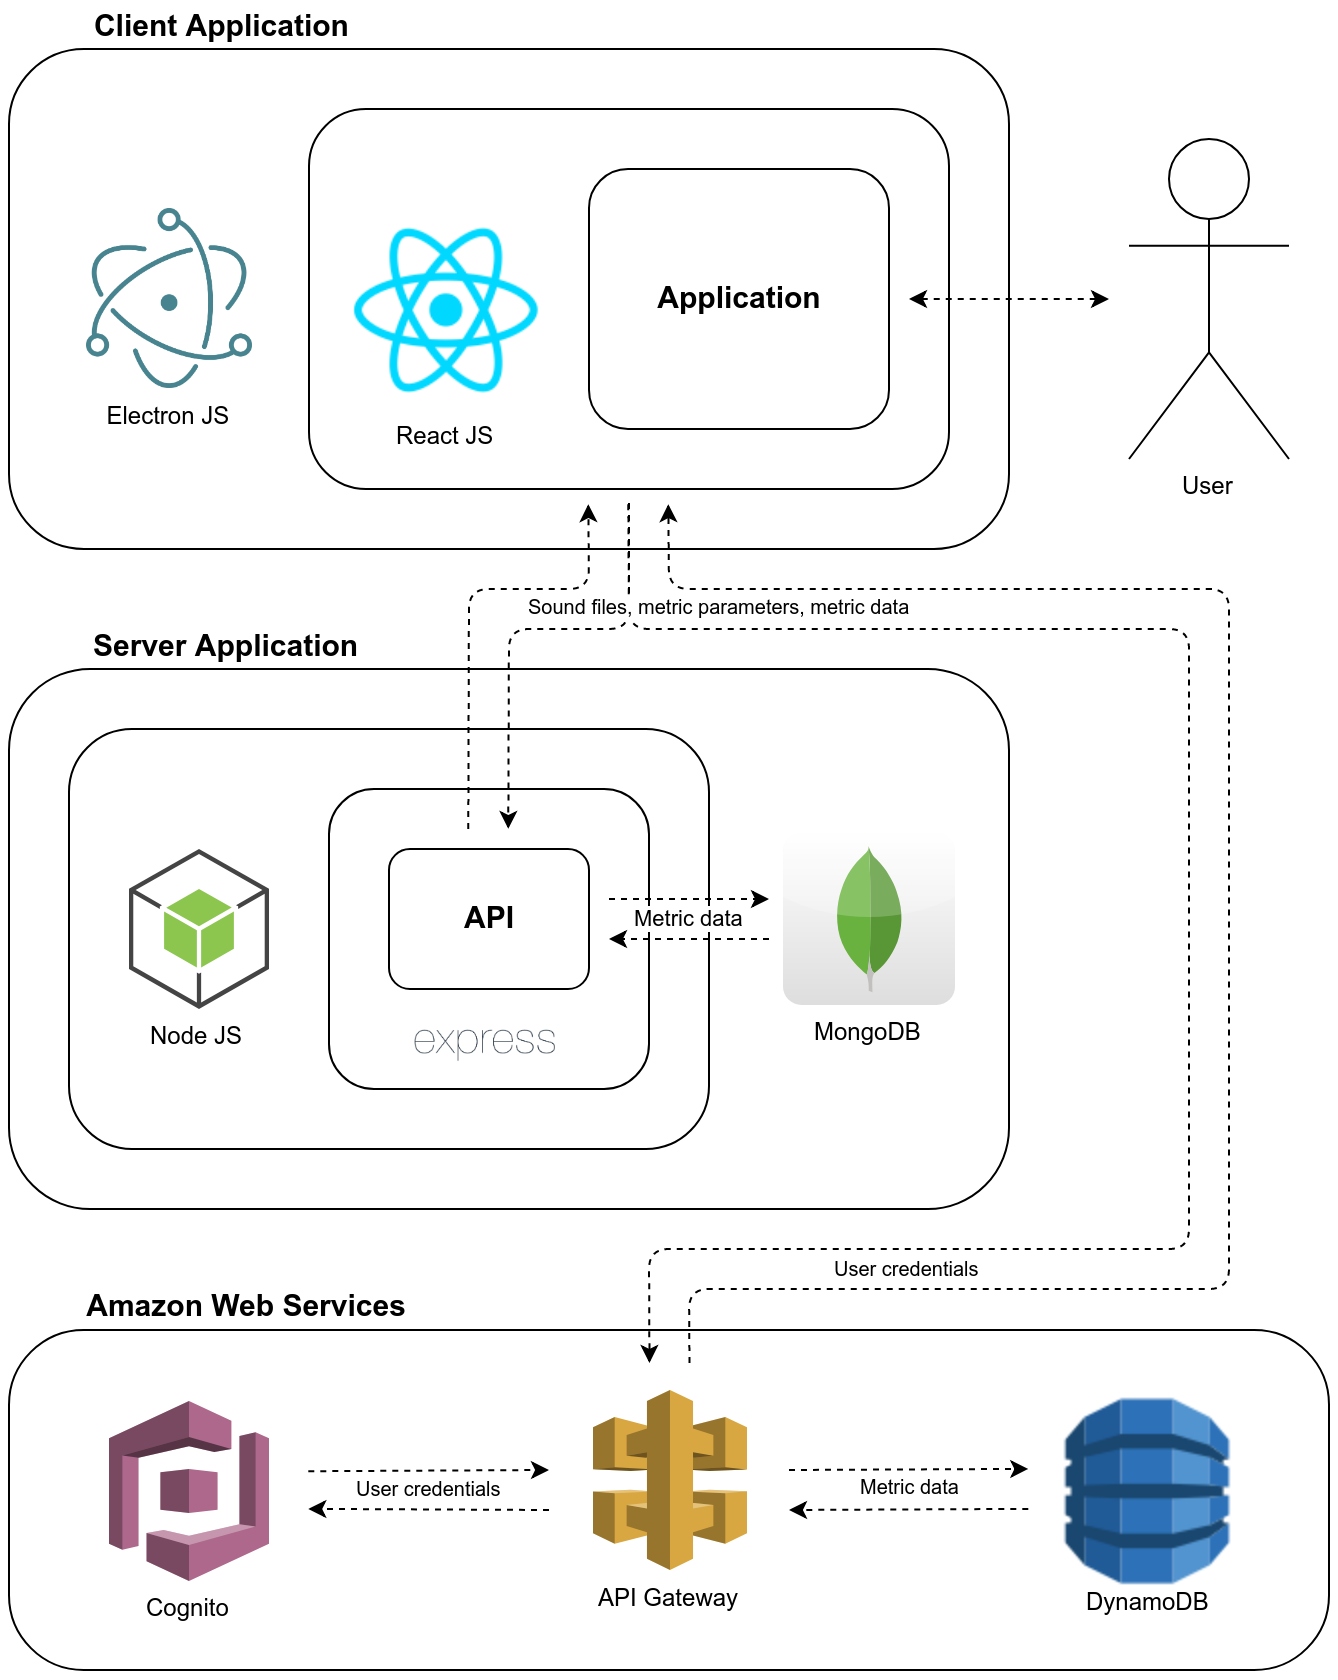
\includegraphics[width=\textwidth]{InfrastructureOverview}
At a high level, the system\textquotesingle s infrastructure is composed of three main parts:
\begin{enumerate}
    \item The \textbf{Client Application}: This contains the user interface with which any users may interact. It runs via an Electron application, and so will be able to run on all major operating systems. Using this application, a user may log into an account, create job requests to process audio files, and present the results of those jobs in a visually accessible manner.
    \item The \textbf{Server Application}: This is where the vast majority of the heavy lifting occurs, including the analysis of audio files for metric data, the storage of the resulting data, and the transmission of any files or data requested by the user via the Client Application. Typically, this application runs on a dedicated server, on which any sound files that are to be analyzed are stored. However, it is equally as possible for the user to run this application and the Client Application on the same machine.
    \item \textbf{Amazon Web Services}: AWS will be tasked with user account management, metric data storage, and intercommunication between Client and Server Applications over the internet. Users that run their own instances of the Server Application will be able to enable data sharing from their own servers, the data from which will be mirrored on AWS DynamoDB, accessible by other users from across the web.
\end{enumerate}

\subsubsection{Front End Infrastructure}
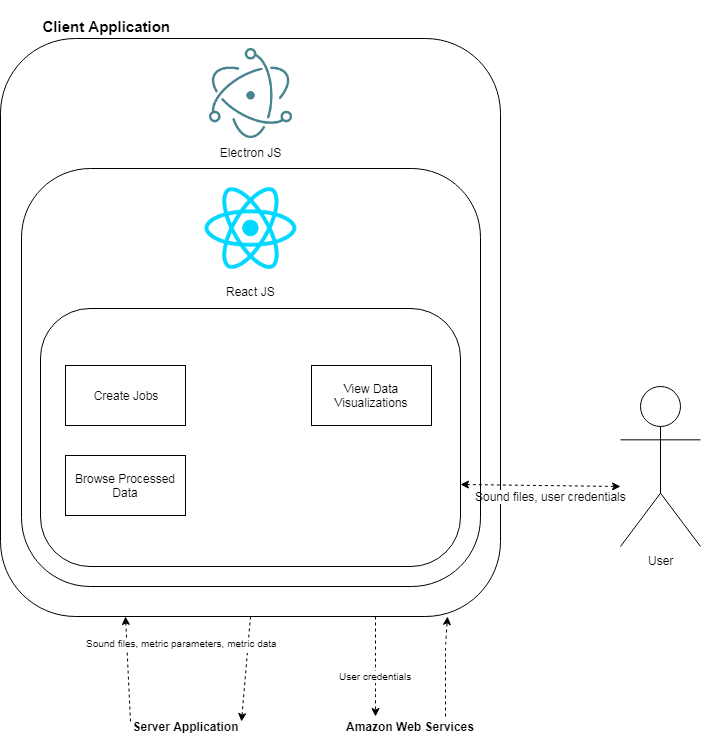
\includegraphics[width=\textwidth]{ClientInfrastructure} \\
The diagram above explains some of the functionality of the client frontend. The specific pages and their design can be seen in the User Interface Specifications section of this report. The frontend is where the user will be spending their time analyzing data and sharing results. The core functionalities of the frontend include creating jobs, browsing processed data, viewing data visualizations, creating public server access for collaboration, and creating research groups.\par
Creating jobs is the process of the user specifying a set of sound files, and the indices and parameters they wish to run on them. As explained in the backend specifications, the outputs are passed to the local database, and used to present the data in visualizations for the user. A user will create a job by selecting sound files whether locally or on their server space, and adding one or more index options and their respective parameters. If the user does not wish to specify parameters, a set of preset values will be used. If the user does not wish to specify an index, then all of the indices will be analyzed. Additionally, the user can create preset index and paremeter sets that they may use frequently, and simply use that set to analyze the data set.\par
As the user analyzes data over time, the results will be stored on the local database, and possibly the remote database should they choose to publish their results for collaboration. Using our service, the user can browse through their processed data to see what analysis they have done on what data sets. From here, they can also look at visualizations.\par
Our service will provide built in data visualization tools. Looking at change of index values over time is important to researchers to see how recent weather events or human interactions have affected the local wildlife. Another visualization available is a line graph, showing the index values by sound file over the whole data set. This is useful to researchers for identifying outliers, as they can easily see which sound files contained a much higher or lower index compared to the rest of the data set. As for collaboration, a geographic heat map is planned to help show where research is being done, as well as the kind of index values being observed at these locations.\par
The more simple side of the front end includes creating research groups and providing public server access. A user can create a research group, making them the admin. They then can add other users to their group, as well as promote members to admin. Research groups allow users access to other members\textquotesingle\ analyzed data and visualizations. As for public server access, our sponsor mentioned how it can be difficult to easily share sound files and data analysis with other researchers across the country. We are going to provide multiple ways for users to do this easily through our service. By implementing OneDrive, Google Drive, and DropBox into our service, users can provide public access folders for hosting sound files and analysis they wish to openly share. In addition, we also will allow users to upload private server credentials that our service will utilize to allow others access to the server for viewing whatever has been made public.

\subsubsection{Local Backend Infrastructure}
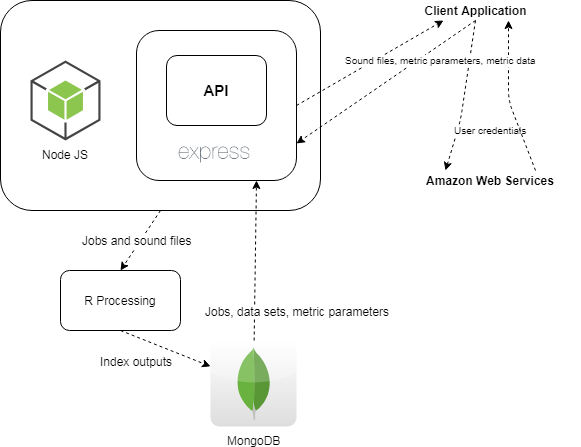
\includegraphics[width=\textwidth]{ServerInfrastructure} \\
This diagram goes into a bit more detail on the local backend. Using Express, our API is constructed to help the backend(s) and frontend communicate, all wrapped in a Node JS application. The front end orchestrates the user\textquotesingle s inputs and jobs to be run, which are then processed in the location the user has specified. This could be a local server that the user has set up using our server side application, or it could be their desktop computer. These jobs and input files go through the R scripts included for analysis in the soundecology package, depending on the user specified indices to be processed.\par
After the analysis is done, the output is different for each index. The MongoDB database we have constructed is set up specifically for storing each index\textquotesingle s output(s). See the database specifications for more a more in depth explanation of that infrastructure.\par
Once the data is stored in the local database, it is then accessible in the user interface on the frontend. We consider this implementation to be perfect for our system, as the local database can be kept on either the user\textquotesingle s desktop or on their server. If the database is hosted on the server, then any other researcher in the network can access this database and see analysis from a peer. This is important for the collaboration requirement made by our sponsor.

\subsubsection{Remote Backend Infrastructure}
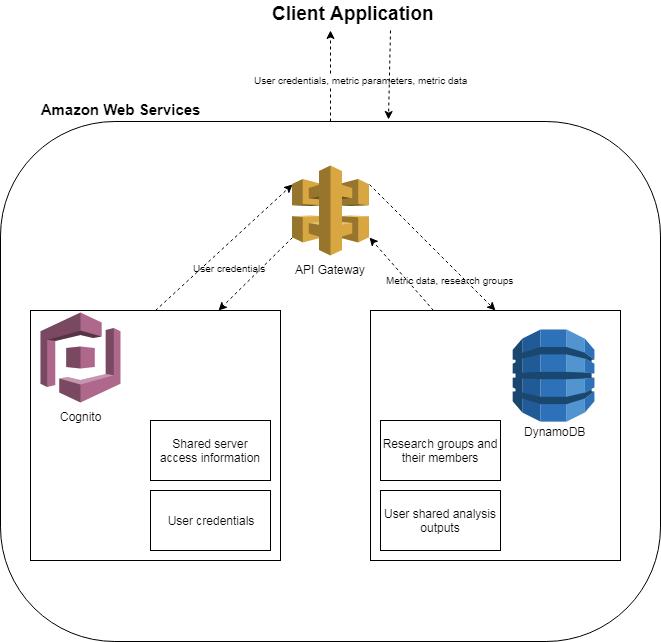
\includegraphics[width=\textwidth]{AWSOverview} \\
Using Amazon Web Services, we can use DynamoDB and Cognito to securely and efficiently manage our users\textquotesingle\ credentials and analysis. Cognito is used for storing user credentials and DynamoDB for research groups and their respective permissions, as well as user shared data.\par
Amazon Cognito is a very useful tool, as it provides a built in interface for users to create accounts as well as log in to existing accounts. These credentials are then stored securely by Amazon to easily create user pools. In addition, Cognito allows for Facebook and Google account log ins, to make account creation easier for the user.\par
DynamoDB is a non relational database, which is useful for us because our local MongoDB database is also non relational. The DynamoDB service will store user shared data analysis that they did on their desktop application. From here, anyone using the service can see that researcher\textquotesingle s analysis. In addition to data outputs, this service will store the user created research groups and their members in order to ensure that users are able to collaborate \textbf{only} with those they wish to.

\subsubsection{Use Case Diagrams}
\begin{center}
    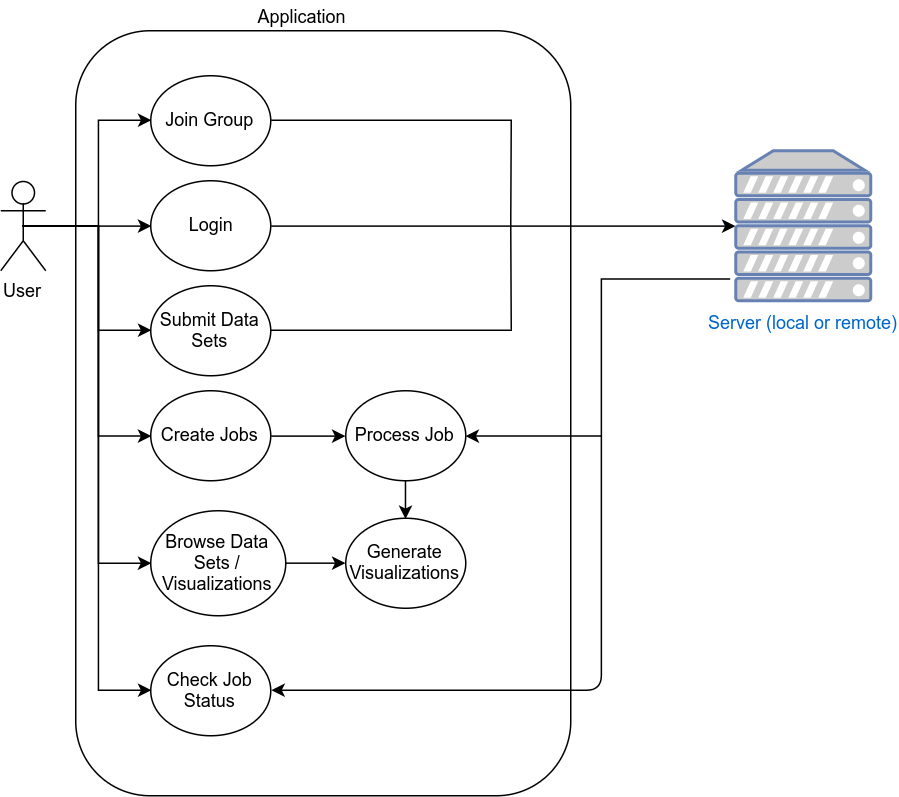
\includegraphics[width=\textwidth]{UseCase}
\end{center}
\newpage
  \section{Front End Design Guidelines}
When working on the user interface, our team mostly tried to adhere to a consistent set of principles. This list was adapted slightly from two separate manifestos to fit the purposes of our project.\par

\begin{itemize}
\item \textbf{The Simplest Option is Usually the Best:} By using what is natively supported by the tools and libraries we have already introduced into the project, the code base can become much simpler to understand amongst team members.
\item \textbf{Reduce the Amount of Moving Parts:} In addition to limitations of dependency introducuction, dependencies should also be reduced as each one can act as a point of failure.
\item \textbf{Understand the Business:} At the end of the day, the code we write only matters in so much as to how it will serve our users (i.e. Dr. Beever and other soundscape ecology researchers). Therefore, it is imperative to have their best interests in mind when working on the end product.
\item \textbf{Do Not Design Systms around Edge-cases:} By simple definition, the amount of times edge-cases occur is insignificant. As a result, the design should first seek to reflect the majority use case and only after should edge cases be adddressed.
\item \textbf{Do Not Make Decisisions Based on Anecodtal Evidence:} By simple definition, anecdotes are generally not representative of reality; they simply reflect the experience of one, single person. So, when proposing a change to the design, data should be collected (generally through testing) to support it, rather than simply listening to the story of a single use case.
\item \textbf{Expect and Acccommodate Change:} The original proposal for this project was intentionally left open ended. It was expected of us to listen to user feedback and think of novel ways to solve some of the problems that the field of soundscape ecology currently faces. Therefore: we must be ready to change the goals and strategies of our endeavors if we wish to succeed.
\item \textbf{Keep Users in Control:} By ensuring that the user interface remains as self-explanatory as possible, users can feel in control of their environment. When users are in control of their environement, they feel more comfortable and are less prone to performing incorrect or irrelevant interactions.
\item \textbf{One Primary Action Per Screen:} By limiting one primary action for each of our pages, users won't become overwhelmed with the many interactions they can make with the application. This was our goal when the front end split into three primary pages: Queue, Catalog, and Settings.
\end{itemize}

  \subsection{User Interface Specifications}
\subsubsection{User Pages}
The user interface is designed to be compact, yet user friendly. The core functions of the interface is to allow the user to log in to the service, view processed data and its analysis, change user settings, create or join a user group, and create jobs to be run on input sets. The more complex pages of this program are explained in the following sections.

\subsubsection{Catalog Page Specifications}
The catalog page is where the user can view their already processed data stored in the backend. If this user is using a shared server, this can potentially also show processed data from \textit{other} users in their group, should those permissions be allowed.\par
The catalog page will be depicted in two separate views, the first involving searching, filtering and selecting jobs and the second, viewing visualizations for the results of the selected jobs. It will usually be the case that users will create a large amount of jobs, corresponding to sets of sound files captured at various locations. Therefore, filtering jobs will be a necessary feature when selecting job results to analyze. The core functionality of the first view is as follows:\\
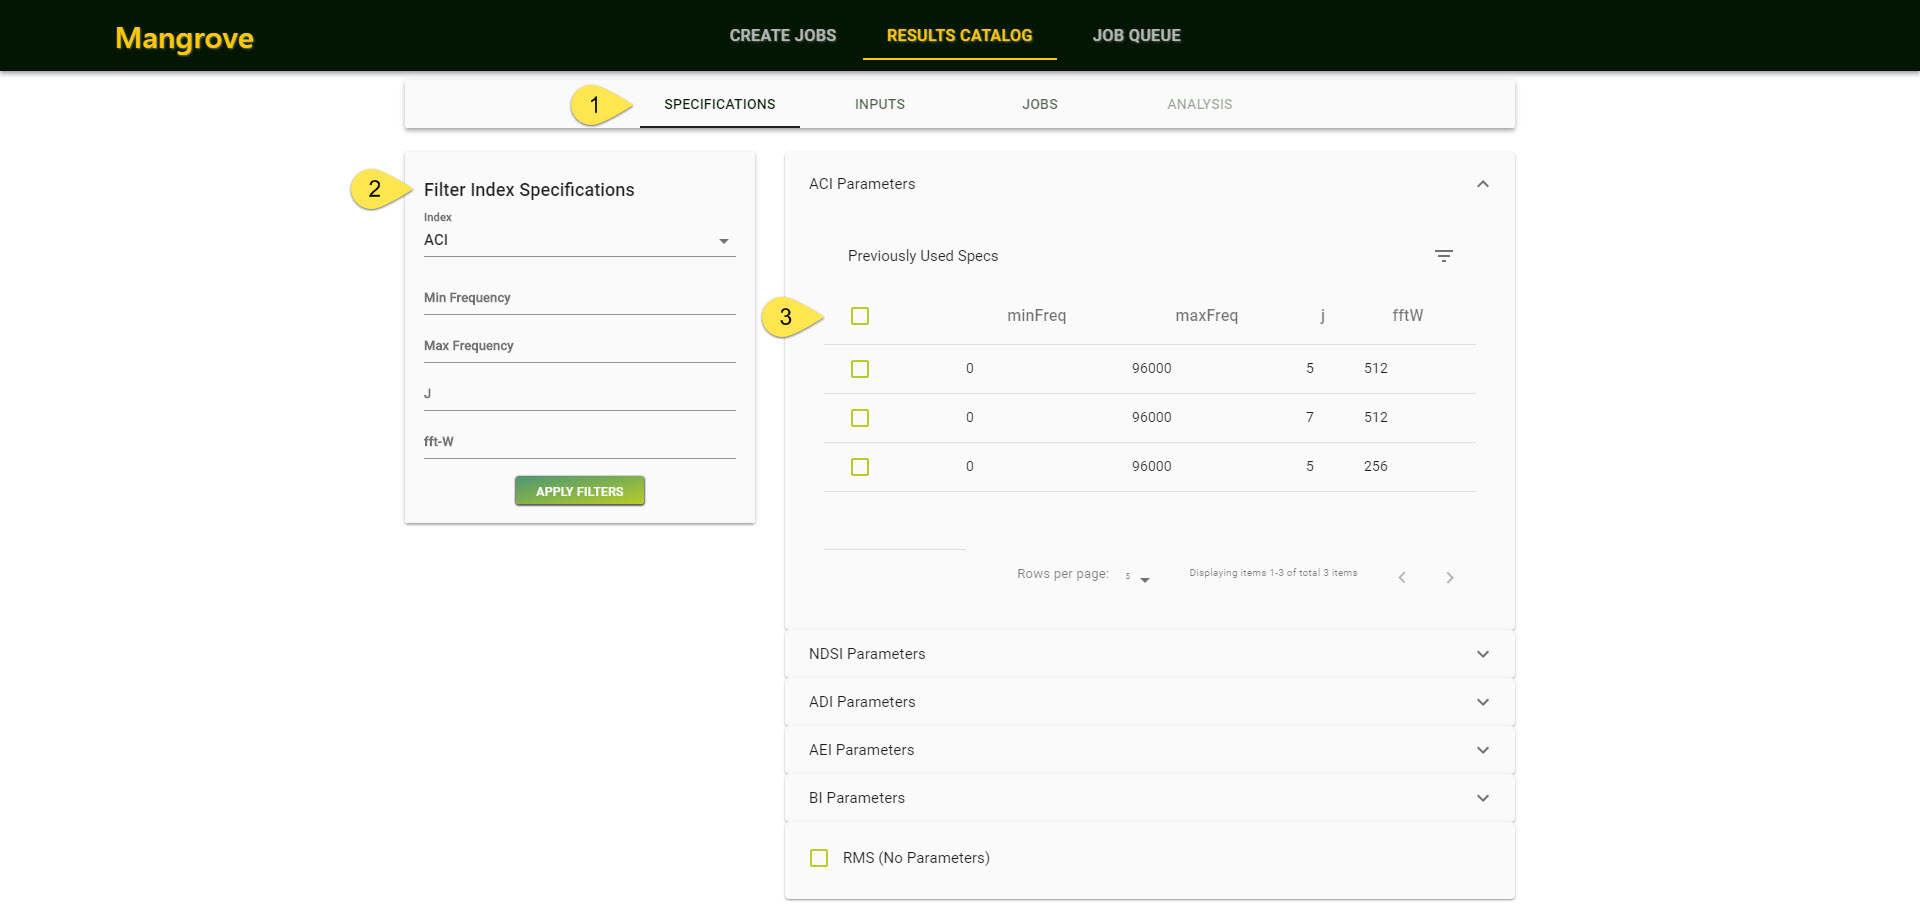
\includegraphics[width=\textwidth]{catalog-1}
\begin{enumerate}
    \item \textbf{Job Searching}\\ The user can search for jobs by site name or tags, which the user can apply to one or many jobs. This feature is helpful if the user wishes to compare results of sound files taken in the same location. An example of searching by a site name, such as \textquotesingle UCF Arboretum\textquotesingle , would show all files captured at that location, provided the user has given the site name as input. Tags will be used to group files in any way that will be relevant to the researcher.
    \item \textbf{Filter By Index}\\ This section consists of a set of checkboxes for each index. They will all be selected when this page is loaded, so that all jobs will be shown to the user at first. Users can uncheck indices as they wish, so that only jobs which were run with checked indices will be listed. Combined with job searching, a user could view results of jobs on files taken in the same location, but analyzed with different indices.
    \item \textbf{Filter By Parameters}\\ This is where a user can specify the parameters used for the jobs which they would like to view analysis. Only parameters for checked indices will be displayed. An example of the usefulness of this feature is when a researcher would like to compare results analyzed within certain frequency ranges.
    \item \textbf{Sorting By Date}\\ Jobs matching the criteria set by the user in the previous sections will be listed with the most recently analyzed jobs shown first. However, the user will be able to show the oldest jobs first or input a specific date range.
    \item \textbf{Filtered Jobs}\\ This is where all jobs matching the filtering and searching done by the user will be listed.
    \item \textbf{View Results}\\ When the user finds the job they would like to visualize, they will click the 'view results' button next to that job. This will open the analysis view of the catalog page and the searching and filtering section will be hidden to allow more room for visualizations.
\end{enumerate}
Some variations to these features will happen if a user belongs to a research group. An option of filtering by jobs that they have created themselves verses themselves and members of their group would be shown. Searching for jobs created by a specific group member would also be permitted in the Job Searching feature.\par
The second view or analysis view of the catalog page focusses on having a clear way for users to view meaningful visualizations of their sound files. The features of the analysis view of the catalog page are outlined below.\par
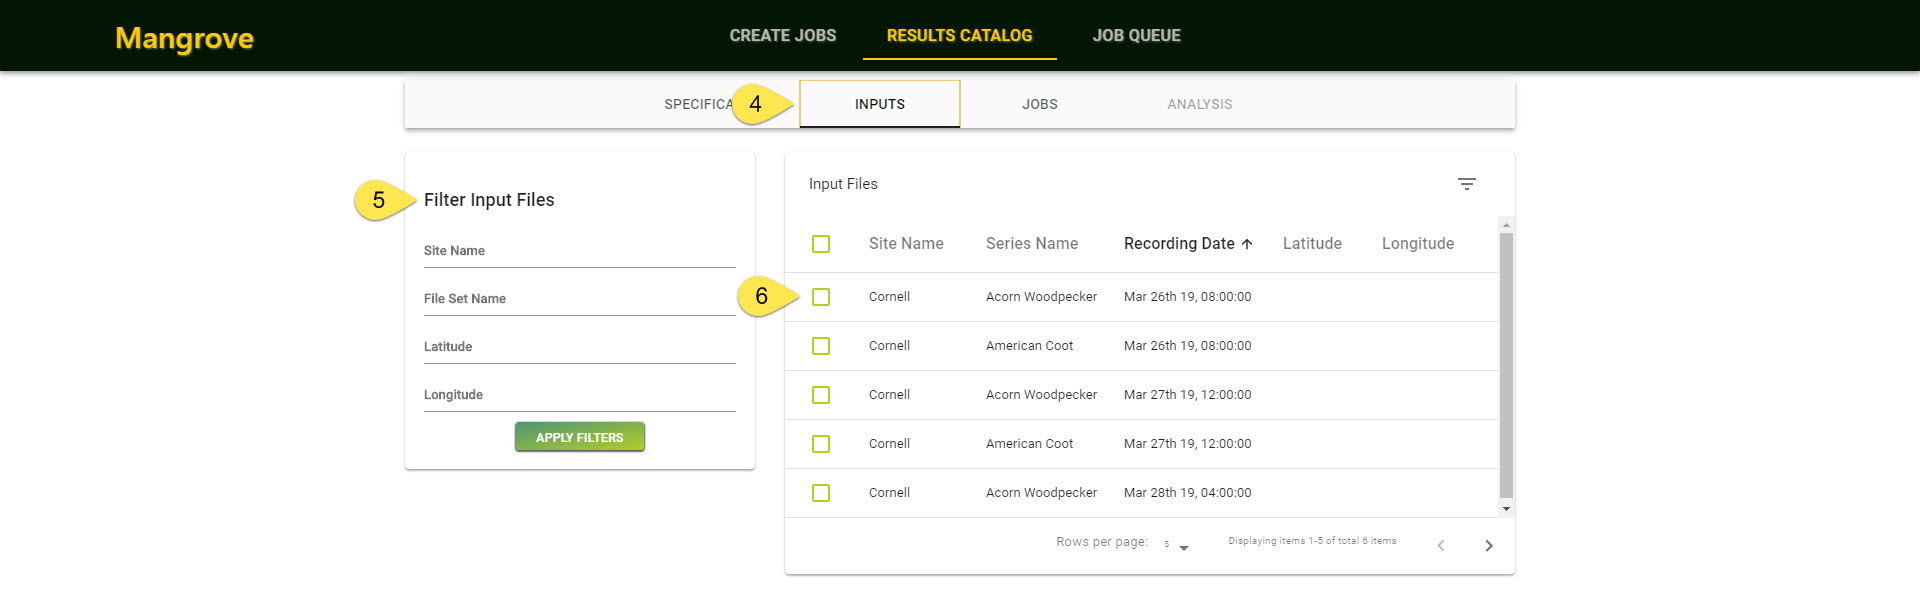
\includegraphics[width=\textwidth]{catalog-2}
\begin{enumerate}
    \item \textbf{Show Filtering Section}\\ If the user wishes to redefine their specifications for the job list, this button can be clicked and will open the previous view.
    \item \textbf{Filtered Jobs}\\ The list of jobs matching the search and filtering specifications set by the user will still be displayed in this view. This section will only take up some of the room on the page and will make the next feature described much easier for users.
    \item \textbf{Compare}\\ If another job of the same index is shown in the filtered job list, the user can click the compare button next to the job. This will overlay both results on the same graph, a feature which will be very useful to researchers.
    \item \textbf{Graph Type Selection}\\ Depending on the parameters and index that was processed, different visualizations will be available. All graphs available for the current index will be listed in this section with radio buttons and the user can select their preferred graph or switch between views.
    \item \textbf{Clear Job}\\ This button can be clicked if the user is finsished viewing the current jobs visualizations. The filtering section will be opened again so a new job can be quickly chosen.
    \item \textbf{View Results}\\ This is where the analysis from the job is shown. Depending on the parameters and index that was processed, different visualizations will be available. If multiple jobs are selected, then a visualization comparing them will be shown.
\end{enumerate}
\subsubsection{Job Creation Page Specifications}
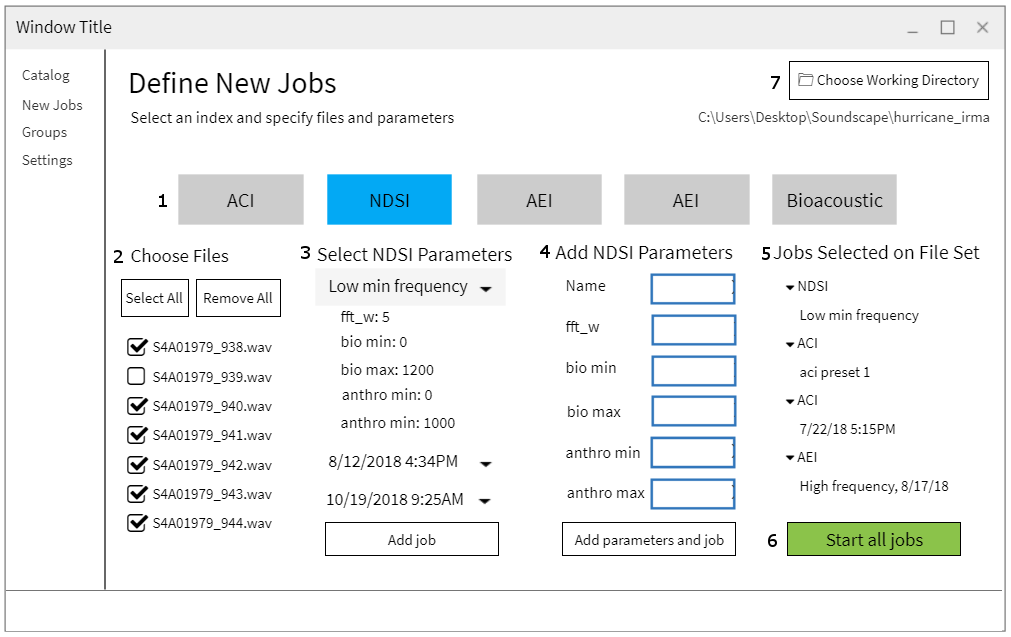
\includegraphics[width=\textwidth]{JobsPage}\\
The jobs page is where the user will select parameters and inputs, and queue jobs to be processed either on their local machine, or on their server where they have the server application running. These jobs and their outputs are then stored in the local database, again either on the local machine or the server, if that is how the user is running the service. The functionality is as follows:\\
\begin{enumerate}
    \item \textbf{Job Index Selection}\\ Each job must have an index to run on the selected inputs. These indices each calculate different data on the input files and are left to the user\textquotesingle s discretion.
    \item \textbf{Input File Selection}\\ This area is populated with related sound files in the current work directory. The user can then selected any of those files they wish to run analysis on. More information on the working directory is found in item 7.
    \item \textbf{Saved Index Parameter Selection}\\ The user has the capability of adding custom preset index/parameter pairs. If the user uses the same index and parameters often, it is useful for them to be able to easily select those options. Any custom saved index/parameter pairs will show here for the user to select. When selected, the user can press the "Add job" button to run the saved index/parameter set on the selected inputs.
    \item \textbf{New Index Parameter Selection}\\ Alternatively, if the user wishes to provide new parameters for the selected index, they can do so here. After selecting the "Add parameters and job" button, the selected index/parameter set will be saved, and the user can either name it for further use, or opt not to, where it will then be named the date and time of creation. Then the service will run the new index/parameter set on the selected inputs.
    \item \textbf{Job Specifications}\\ Here the current set of jobs that the user has defined on the input set are shown. The name of the index and the chosen parameters are shown for each specified job. The user can remove any of these jobs at their discretion.
    \item \textbf{Start All Jobs}\\ As the user creates jobs on selected inputs, they will be added to a queue. When the user is ready, they will select this button to run the chosen jobs in item 5 on the selected inputs in item 2.
    \item \textbf{Working Directory}\\ The working directory is where the service will look for chosen input files. This is an important aspect of the service, as the user may be working on a server where sound files are frequently moved. The user can specify where they would like to grab sound files from whenever they want, without having to worry about files being moved. If files are moved, the service will return an error stating that the file could not be found, and to change the working directory as needed.
\end{enumerate}
\subsubsection{Job Queue Page Specifications}
The Job Queue page helps the user see the status of jobs started using the Job Creation page. A job has five possible statuses, including finished, failed, cancelled, queued, and processing. These, along with the functionality of the Job Queue, are shown in the image below.\\
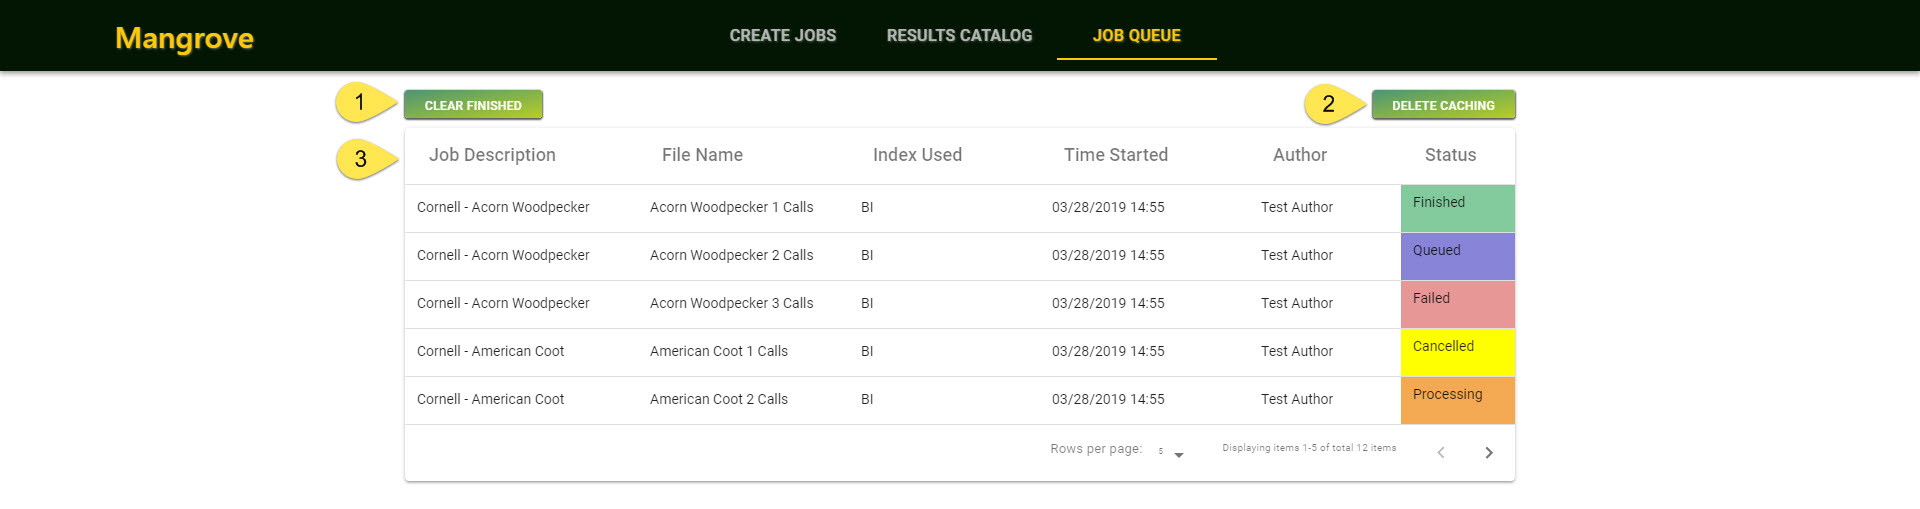
\includegraphics[width=\textwidth]{jobQueue}
\begin{enumerate}
  \item \textbf{Clear Finished}\\ This button allows the user to remove any jobs with the finished status. This helps clean up the job queue and show only those jobs that are waiting to be processed, or are in the process of doing so, or those that failed.
  \item \textbf{Delete Caching}\\ This button will remove all jobs in the job queue regardless of status. This button is more to be used as an error handler, if some error occurs during processing.
  \item \textbf{Job Queue}\\ The actual queue itself is organized as a table containg a job description of the site and series, author, and the file name itself. Additionally, the index being used in the job and the time started are available. Finally, the job status is color coded in the last cell.
\end{enumerate}

\subsubsection{Login Page Specifications}

\includegraphics[width=\textwidth]{login}\\
The login page is pretty straightforward. Users will create accounts with their email or may choose to log in with their gmail account. A password reset can be emailed to the user if they forgot their password. This page will also feature a logo that represents our application. Information about what the application does and available features can also be found on this page.\par


  \subsection{User Interface Design}
When designing an interface, the purpose of the service comes into question. It is important to define what drives each page of the application, and what the core functionality of it is in order to choose the best layout and color scheme for the component\textquotesingle s representation and the user\textquotesingle s accessibility. In addition, identifying the core user base is also important in designing the interface.

\subsubsection{Interface Color Selection}
For this service, some pages are visually driven, with little text on the screen, while some are text driven. The Catalog page for instance relies on the data visualization component as the main focal point, while the settings page contains only text. This presents a bit of a conflict as to which colors to choose for a service wide color palette.\par
With pages that are mainly visually driven, like the Catalog page, it is best to use darker background colors to help the visuals stand out compared to the rest of the page. For text however it is best to use lighter color backgrounds as to not cause strain on the reader\textquotesingle s eyes. Thus it is decided that the service will be mostly light colored backgrounds, with some colored components.\par
For the Catalog page, it is important for the data visualizations to stand out. Contrast in pages is important for drawing attention to elements and directing the user\textquotesingle s eyes. The analysis section of the page should have a background color to make it stand out against the rest of the page.\par
As for the actual color palette selection, our sponsor has a logo made up for his research that contains core colors of yellow and black. We liked this logo from the get go and wanted to incorporate these colors into the application. We aim to follow the 60-30-10 rule using a palette of white yellow and black.

\subsubsection{Page Organization}
Page organization is important for putting elements in a logical and meaningful place. Placing related content together helps the end user be more efficient, especially on pages like the Job Creation page. The following thought process went into each page.\par
The Catalog page contains the user\textquotesingle s results from past jobs, and allows them to filter through them and view the analysis for whichever they\textquotesingle d like. The main component of this page is again the data visualizations, so it is important that this component take up most of the space on the page. The side components, that being the filtering section and the results table, take up a third of the screen and are aligned to the left, while the data visualizations take up the other two thirds and the right side of the screen. This helps to divide up the content for the user, and make filtering and navigating the results table easier.\par
The Settings page acts as a standard panel for global application preferences. This is implemented as a simple form primarily consisting of three components: Account Settings, Group Server Access, and Processing. The Account Settings component allows users to change both their email addresses and passwords associated with their accounts. The Group Server Access component lists information (role, IP address, and login credentials for the server) on each of the remote servers associated with a user\textquotesingle s account and allows them to modify it (with respect to their role). In addition, for each remote server, the component also allows the user to invite new members to the group by providing their email. The Processing component is a simple list of radio buttons to specify which server the user currently wants to process jobs with.\par
The Job Creation page is where users will define and start jobs on their sets of sound files. The organization of this page is based on the step by step process of starting jobs. When a user first visits this page, they will see a group of buttons which are used to select the index that the analysis will use. On loading the page, they will also see a button to change their working directory and a list of wav files contained in the current working directory. A user could either choose an index or specify the files they would like to analyze as the first action. Once the index and files have been specified, the stepper component will move to the next step and the parameter specification components will become visible. The use of a Stepper component will make sure the user is clear on all steps that need to be taken to successfully start a job. When all required information has been inputted, the user will be free to start the job. After starting the job, the user will be notified that it started successfully and will be given the option to navigate to the In Progress Jobs page, to view the state of jobs not yet completed. If the user would like to start a new job, the set of files previously analyized will remain selected for ease of use, as it is common to run multiple indices on the same files.\par

\subsubsection{Page Use Cases}
\begin{center}
  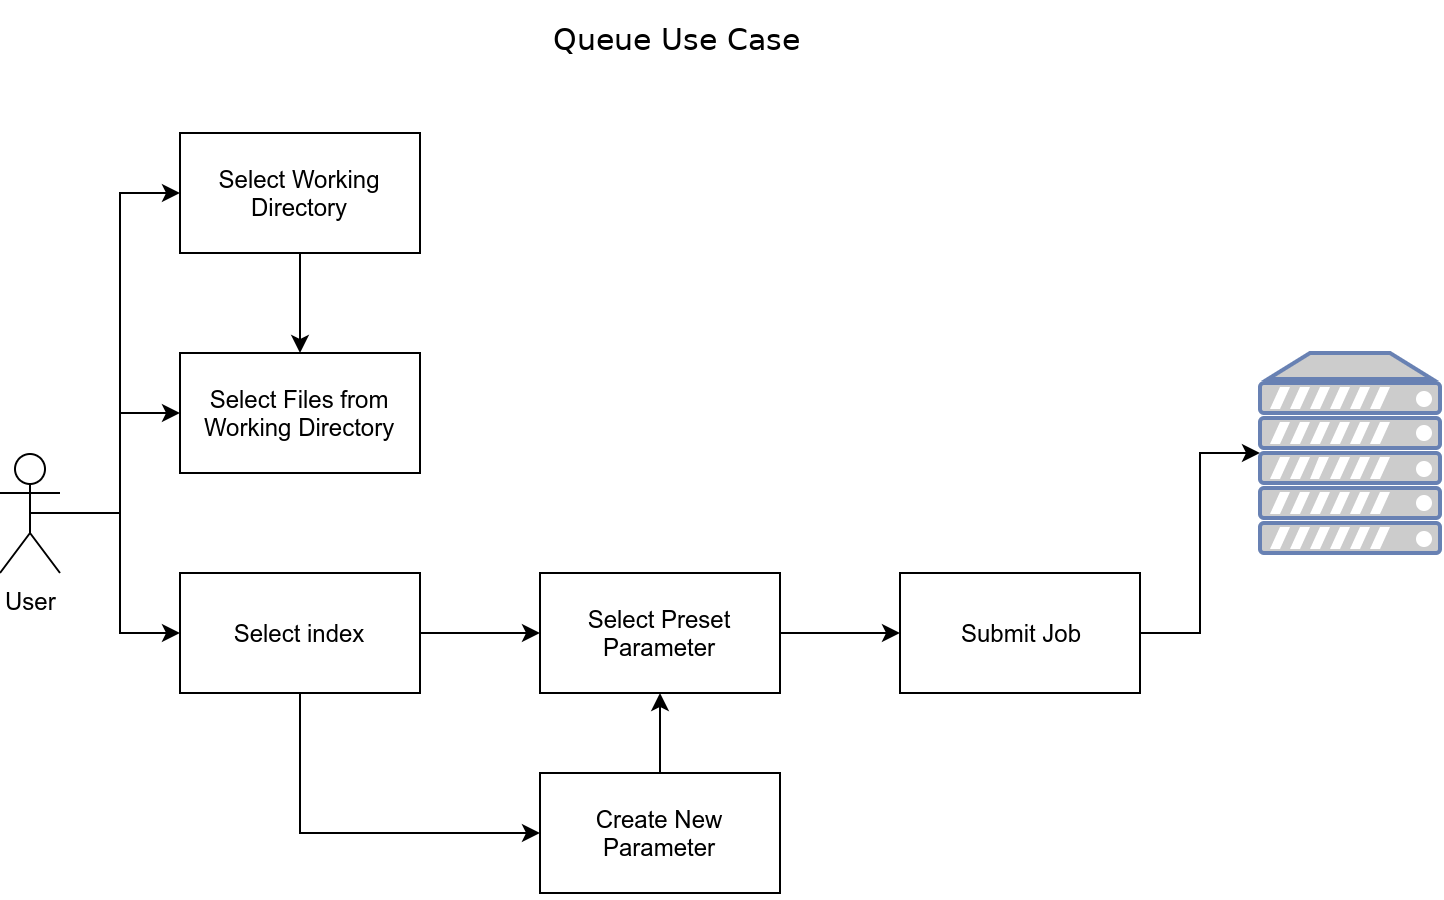
\includegraphics[width=\textwidth]{UsecaseQueue} \\[12pt]
\end{center}
\begin{center}
  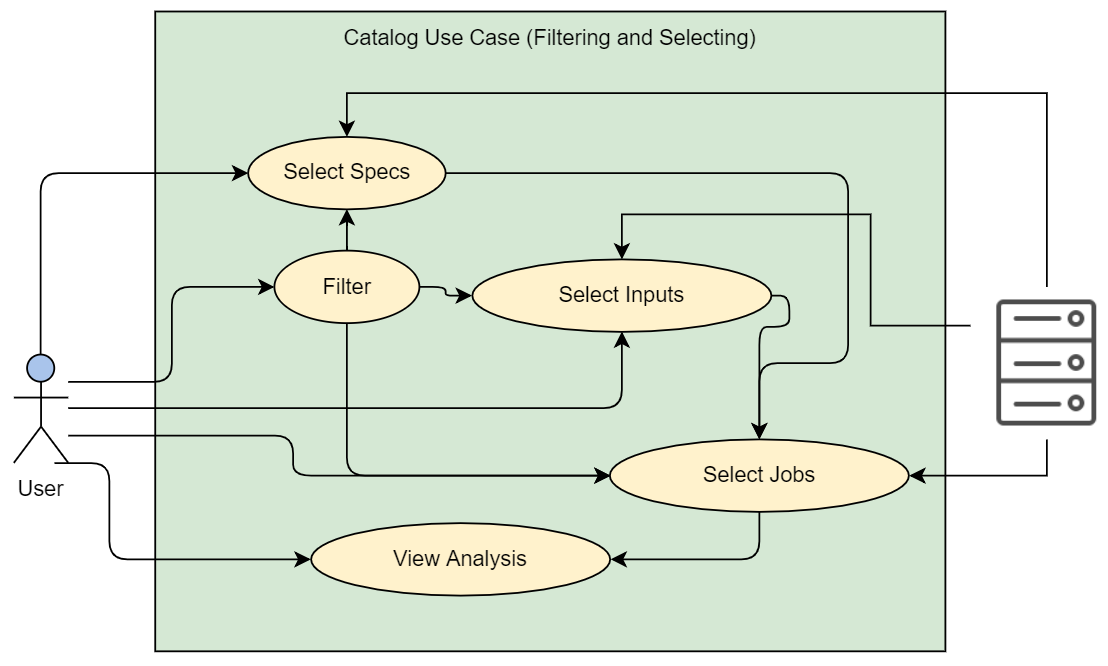
\includegraphics[width=0.85\textwidth]{UsecaseCatalog} \\[12pt]
\end{center}
\begin{center}
  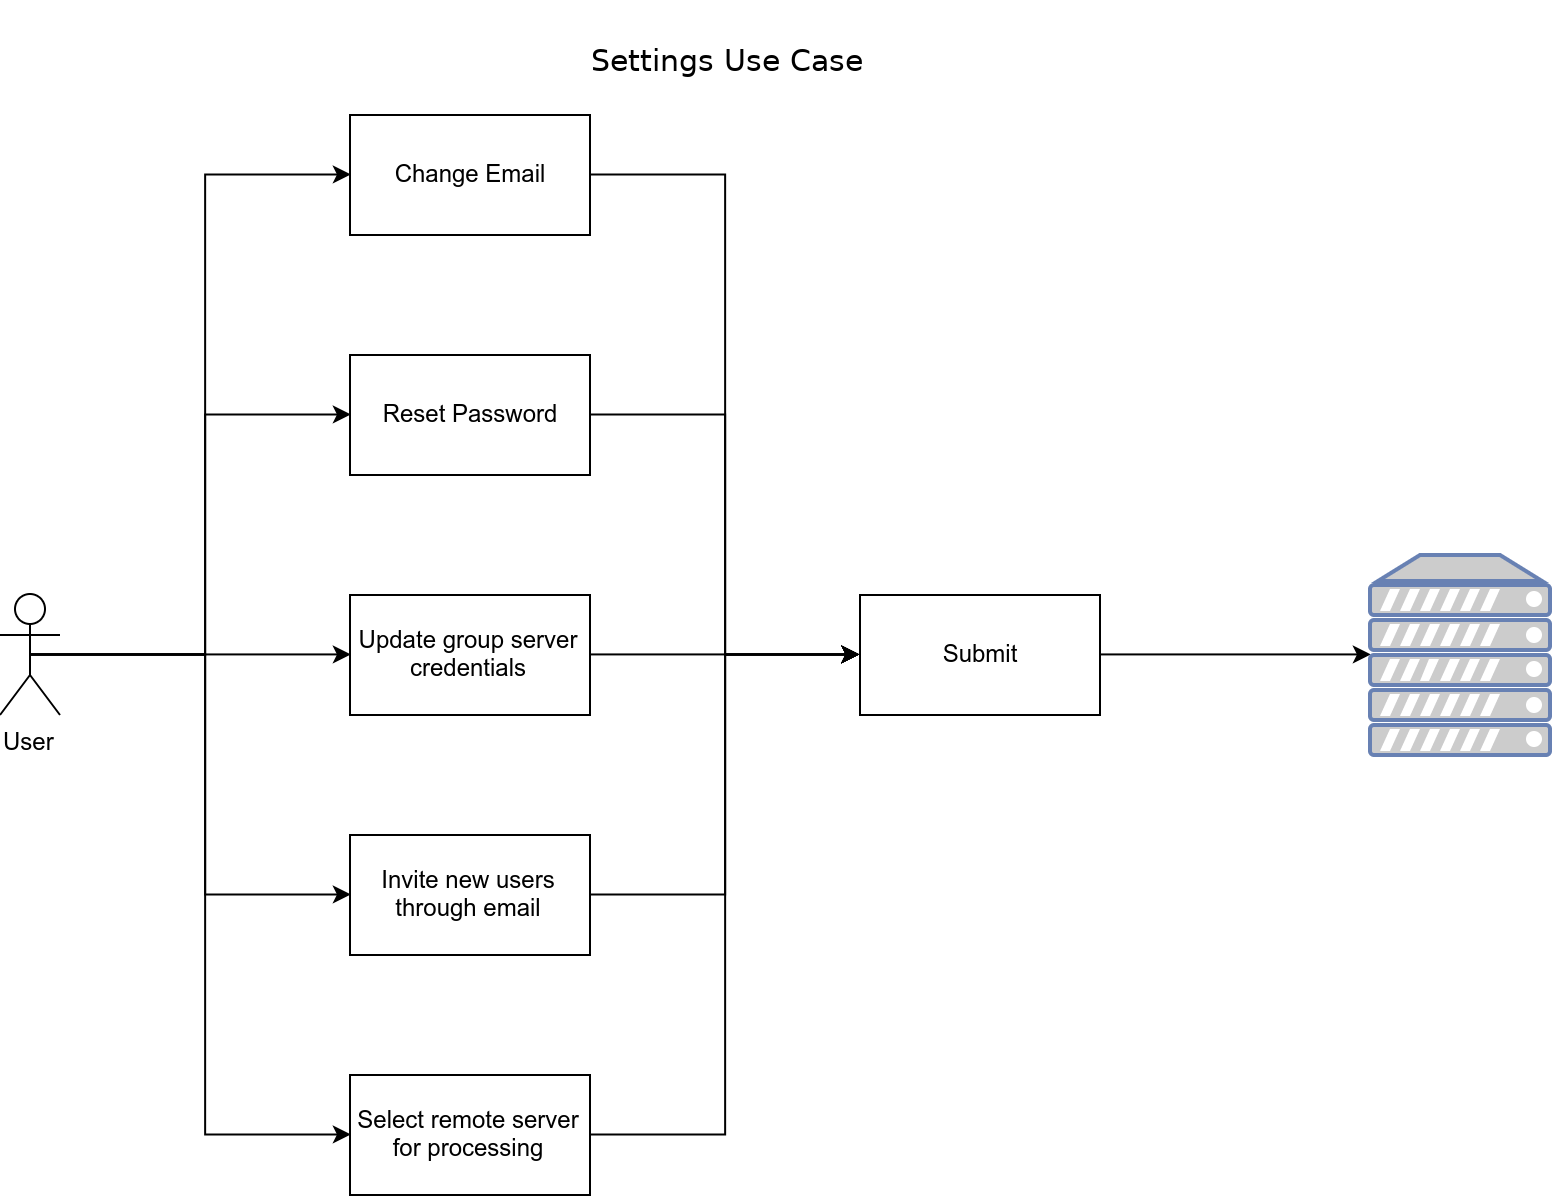
\includegraphics[width=\textwidth]{UsecaseSettings} \\[12pt]
\end{center}

\subsubsection{Frontend Frameworks}
A big part of getting the front end of the service up and running as quickly as we did was the use of frameworks. The core frameworks for this project are explained in the Infrastructure section of this project, so this will only cover the core frontend frameworks. The core frameworks used are as follows:
\begin{itemize}
  \item Material-UI
  \item Bootstrap
  \item Recharts
\end{itemize}
Material-UI is a framework for React that includes new components to easily add into the existing pages, handling styling for these components to help save time in development. This framework is used heavily in both the Catalog and Job Creation pages.\par
Bootstrap is a CSS framework made to handle screen size changes without hassle on the developer\textquotesingle s end. Bootstrap divides the page up into twelve parts, containing rows and columns. Components can then be placed into their respective rows and columns, including nesting, to create a functional and dynamic interface. This framework is especially useful for us to handle changing screen sizes.\par
For the analysis part of the Catalog page, we needed a framework to turn our JSON data into graphics based on the user selected result from the result table. Recharts is a framework for doing just that, and is in charge of creating the respective data visualizations for each index. Recharts provides easy to use code made specifically for React to turn our data into nice, concise graphics.

  \subsection{Creating Flexible Data Visualizations}
\subsection{Data Visualization Research}

\subsubsection{Line Charts}

\begin{htmlcode}
<LineChart width={900} height={600} data={data} >
  <CartesianGrid strokeDasharray="3 3"/>
  <XAxis dataKey="name" label={xLabel}/>
  <YAxis label={yLabel}/>
  <Legend />
  <Tooltip/>
  <Line type='natural' dataKey={firstDataKey}
                      stroke='#8884d8'
                      dot={false} />
  <Line type='natural' dataKey={secondDataKey}
                      stroke='#82ca9d'
                      dot={false} />
  <Brush />
</ LineChart>
\end{htmlcode}

The code above is used for creating the line charts seen in the NDSI, ACI, and Bioacoustic index. This flexibility is allowed as we can pass the label names and data key parameters through the components depending on which index was chosen.\par

\begin{htmlcode}
<ReferenceLine y={adiLeft} label="ADI Left" stroke="#433eaf"/>
\end{htmlcode}

For the ADI and AEI indices, a reference line is included as well, which is elaborated on more in the Data Visualization Research section of this paper.

\subsubsection{Bar Graphs}

\begin{htmlcode}
<BarChart width={900} height={600} data={graph1}>
  <CartesianGrid strokeDasharray="3 3" />
  <XAxis dataKey="name" label="Channel"/>
  <YAxis label="Value"/>
  <Tooltip />
  <Legend />
  <Bar dataKey="ndsi" fill="#8884d8" />
  <Bar dataKey="biophony" fill="#82ca9d" />
  <Bar dataKey="anthrophony" fill="#e79797" />
</ BarChart>
\end{htmlcode}

The NDSI bar charts are a bit more complicated to make flexible. One of the NDSI charts includes three different bar groups, while the other only includes two. So, making one all encompassing React component is out of the question. Thus, the code above is used for the three bar group visualization, with similar code used for the two bar graph visualization.

\subsubsection{Area Graphs}

\begin{htmlcode}
<AreaChart width={900} height={600} data={data} >
  <CartesianGrid strokeDasharray="3 3"/>
  <XAxis dataKey="name" label={xLabel}/>
  <Legend />
  <YAxis label={yLabel}/>
  <Tooltip/>
  <Area type='monotone' dataKey={firstDataKey}
                        stackId="1"
                        stroke='#8884d8'
                        fill='#8884d8' />
  <Brush />
</ AreaChart>
\end{htmlcode}

The area graphs are also very flexible, as they are not used as much in this service. Thus, using the code above, we can easily include area graphs wherever they are needed regardless of the index (which is only Bioacoustic index) by again passing parameters through components.


  \subsection{Database Design}
\subsubsection{Database Overview}
\begin{center}
  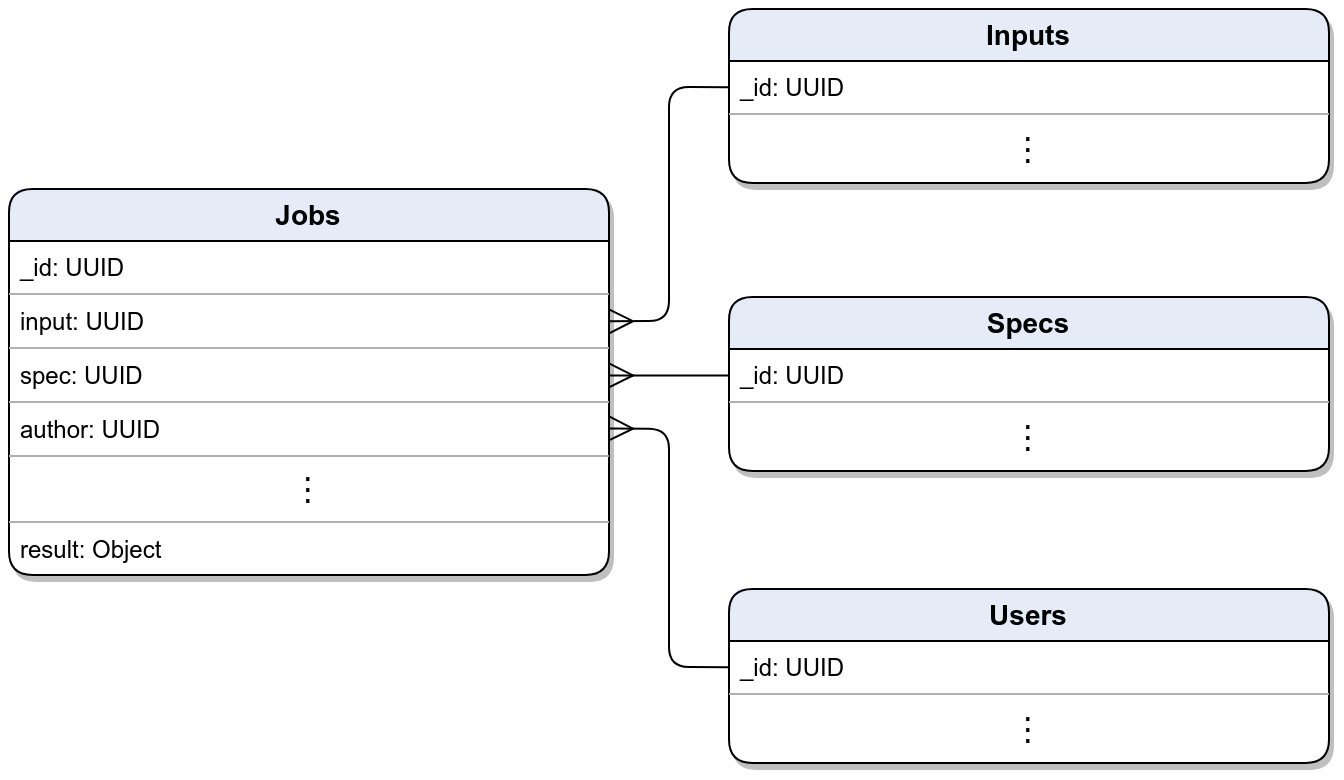
\includegraphics[width=\textwidth]{DatabaseOverview} \\[12pt]
\end{center}
The diagram above represents the database implementation that will be used in
the server application at a high level---more detailed representations will
follow in the sections below. Note that while this is an entity-relationship
diagram (ERD), a type of diagram normally used to represent relational databases, a non-relational database (MongoDB) will be used for this application in conjunction with AWS Cognito to hold user account information. The ERD, while an imperfect representation for a non-relational database, simply provides a convenient way of demonstrating the format in which information will be stored in collections and the ways in which these collections will relate to one another.\par
There are three collections that will be used to store all information in the database: Jobs, Inputs, and Specs, while Users will be stored in a Cognito User Pool. The Jobs collection is at the core of the design, as Jobs are where the action happens. This collection contains the UUID\textquotesingle s of each relevant document from other collections, metadata about each Job, and, upon completion of the Job, the resulting output from the analysis performed. The Inputs collection contains information about the WAV audio files to be processed by each Job, including the location in which each of the files is stored on the server. The Specs collection holds information about how to process each Job, namely, the list of parameters needed for each metric to be run. The Users ``collection'' (a Cognito User Pool) contains information necessary in keeping track of users.\par
The database is implemented using Mongoose, which allows for a schema-based object modeling approach to designing the MongoDB database and validating its documents. Mongoose\textquotesingle s capabilities play a vital role in the database implementation, as the object modeling features allow for inheritance between schemas, and this can be seen in both the Job and Spec models as shown in the next section.

\subsubsection{Jobs, Inputs, \& Specifications}
\begin{center}
  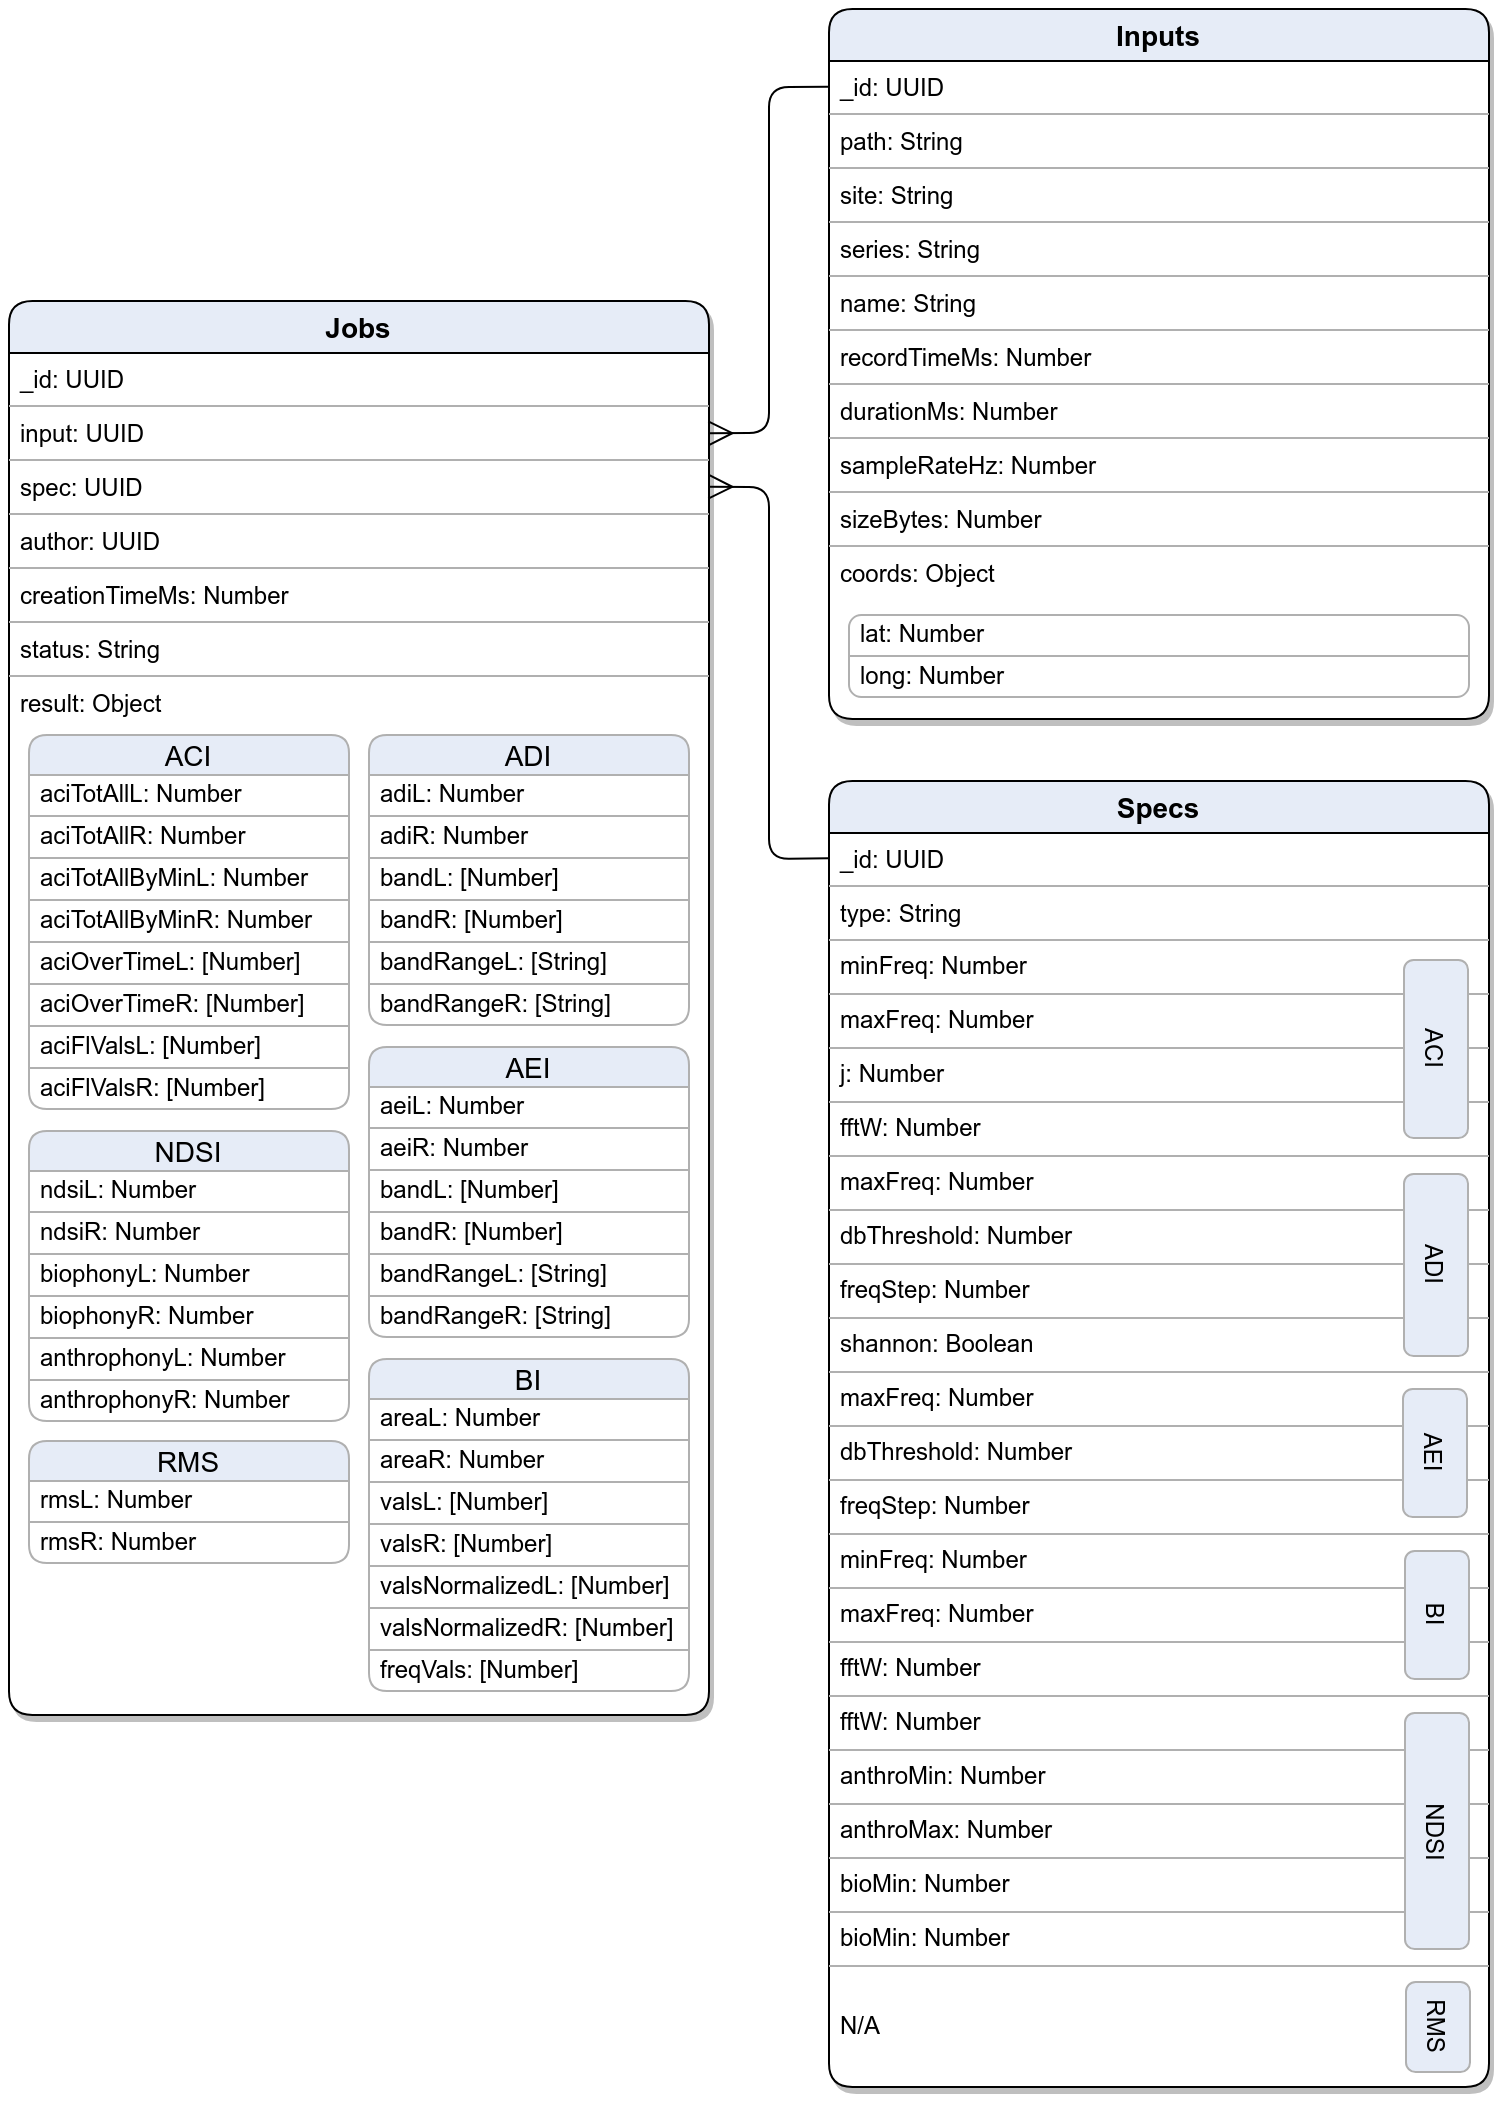
\includegraphics[width=\textwidth]{DatabaseJobs} \\[12pt]
\end{center}
It should be clear from the diagram that the database design is focused around the Jobs collection, and this makes sense given that Jobs are where the action takes place. The Jobs collection connects to the Inputs, and Specs collections via the UUID\textquotesingle s of a document from each of these being stored in each Job document. Additionally, the metadata of when each Job was initially created is stored in \codesnip{creationTimeMs}. The \codesnip{status} of each Job is an enumerative String that may hold one of the following values: \codesnip{"queued"}, \codesnip{"processing"}, \codesnip{"finished"}, \codesnip{"failed"}, or \codesnip{"cancelled"}. Upon the completion of the processing phase of a Job (marked by a \codesnip{status} of \codesnip{"finished"}), the \codesnip{result} Object will be populated with the results of each \codesnip{type} of Job. The possibilities for each Job\textquotesingle s \codesnip{result}, based on the \codesnip{type} of Spec used, can be seen above.\par
It is important to note the way in which the different types of Jobs are able to be stored in the same collection, as differences in Job type contain variations on the Objects stored in the \codesnip{result}. This is done by a Mongoose\textquotesingle s feature called a \textit{discriminator}. Discriminators are what enable inheritance between different Mongoose models, and in both the Job and Spec models, they are used to define each ``child'' model. For example, while we have the ``parent'' model of Job, we also have the AciJob, NdsiJob, and so on, that inherit from it. Likewise, a similar approach is taken with the Spec models. The result is that each child model is stored in the same collection as those that share the same parent, and this provides the benefit of being able to regard only that collection when pulling information from the database.\par
The Specs collection represents the parameters used in each Job. These parameters are specific to each metric being calculated by the Job. Keeping these parameters separate from each Job allows for reusability in the sense that if a user wants to run the same parameters on multiple inputs, all he or she must do is create an identical Job with a different input, rather than defining the parameters each time.

\subsubsection{Users \& Groups}
\begin{center}
  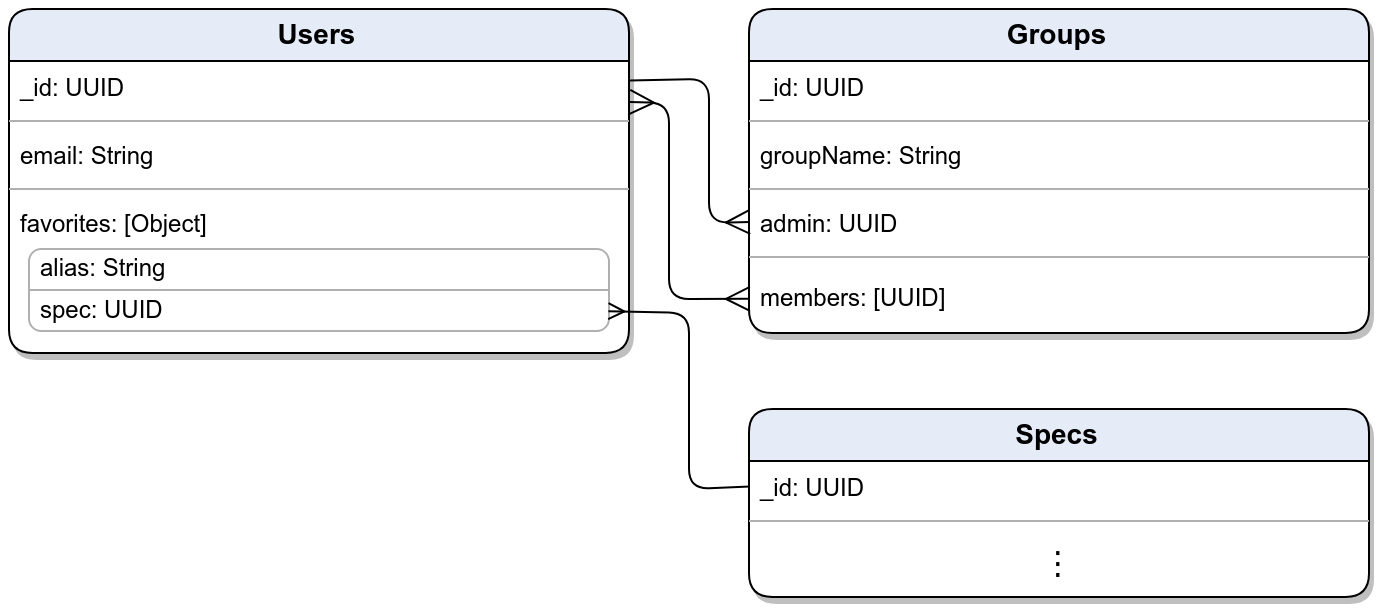
\includegraphics[width=\textwidth]{DatabaseUsers} \\[12pt]
\end{center}
While the heavy-lifting of user authentication will be handled by AWS Cognito, it can still be useful to store some pieces of user data in the database. For example, once authenticated, a user then has access to his or her list of favorite specifications, which can be used in the client application to simplify the creation of new Jobs. The Users collection is where this kind of information will be stored.\par
Users can also be a part of one or more groups, or create a group. If a user creates a group, they are added as the admin of the group. An admin of a group can then add more users to also be admins. Groups have a list of members as well, and this references the Users collection.\par

  \subsection{Application Programming Interface}

% Use these for correct spacing after each paragraph header (notice the \mbox{}\\[\Xheaderspace] )
\newcommand{\tabularheaderspace}{6pt}
\newcommand{\longtableheaderspace}{-22pt}
\newcommand{\codeheaderspace}{-21pt}

% General table formatting
\newcommand{\fieldcolwidth}{3.2cm}
\newcommand{\typecolwidth}{1.9cm}
\newcommand{\metriccolwidth}{1.9cm}
\newcommand{\desccolwidthlg}{8.8cm}
\newcommand{\desccolwidthsm}{6.4cm}
\newcommand{\errconditioncol}{5.5cm}
\newcommand{\errcodecol}{0.8cm}
\newcommand{\errbodycol}{7.6cm}
\newcommand{\cellpaddingvertical}{1.05}
\newcommand{\reqhead}[1]{\bfseries \cellcolor{codebg} #1}
\renewcommand\cellalign{lc}

% API request listings
\subsubsection{Search Inputs}
Search for inputs that match a specified description.

\paragraph{GET} \mbox{}\\[\codeheaderspace]
\begin{htmlcode}
https://<base-url>/search/inputs
\end{htmlcode}

\paragraph{Header} \mbox{}\\[\longtableheaderspace]
\begingroup
\renewcommand{\arraystretch}{\cellpaddingvertical}
\begin{longtable}{| m{\fieldcolwidth} | m{\typecolwidth} | m{\desccolwidthlg} |}
  \hline
  \tablehead{Field}
  & \tablehead{Type}
  & \tablehead{Description}
  \\ \hline

  \codesnip{Content-Type}
  & String
  & \codesnip{"application/json"}
  \\ \hline
\end{longtable}
\endgroup

\paragraph{Request Body Fields} \mbox{}\\[\longtableheaderspace]
\begingroup
\renewcommand{\arraystretch}{\cellpaddingvertical}
\begin{longtable}{| m{\fieldcolwidth} | m{\typecolwidth} | m{\desccolwidthlg} |}
  \hline
  \tablehead{Field}
  & \tablehead{Type}
  & \tablehead{Description}
  \\ \hline

  \codesnip{path}
  & String
  & The path to the input file on the host machine, from the root input folder. Note: This will always be a path to a WAV file.
  \\ \hline

  \codesnip{site}
  & String
  & The name of the site in which the input was recorded.
  \\ \hline

  \codesnip{series}
  & String
  & The name of the series of recordings that the input is a part of.
  \\ \hline

  \codesnip{recordTimeMs}
  & Object
  & The time at which the input audio file was recorded, listed in milliseconds since the Unix epoch.
  \\ \hline
  \hspace{3mm} \codesnip{min}
  & Number & Minimum value of \codesnip{lat}. \\ \hline
  \hspace{3mm} \codesnip{max}
  & Number & Maximum value of \codesnip{lat}. \\ \hline

  \codesnip{coords}
  & Object
  & The coordinates of the location in which the input was recorded.
  \\ \hline

  \hspace{3mm} \codesnip{lat}
  & Object
  & The latitude of the recording location.
  \\ \hline
  \hspace{6mm} \codesnip{min}
  & Number & Minimum value of \codesnip{lat}. \\ \hline
  \hspace{6mm} \codesnip{max}
  & Number & Maximum value of \codesnip{lat}. \\ \hline

  \hspace{3mm} \codesnip{long}
  & Object
  & The longitude of the recording location.
  \\ \hline
  \hspace{6mm} \codesnip{min}
  & Number & Minimum value of \codesnip{long}. \\ \hline
  \hspace{6mm} \codesnip{max}
  & Number & Maximum value of \codesnip{long}. \\ \hline
\end{longtable}
\endgroup

\paragraph{Example Request Body} \mbox{}\\[\codeheaderspace]
\begin{jsoncode}
{
  "path": "fileName.wav",
  "site": "UCF Arboretum",
  "series": "Hurricane Irma",
  "recordTimeMs": {
    "min": 1504929600000,
    "max": 1505102400000
  },
  "coords": {
    "lat": {
      "min": 28,
      "max": 29
    },
    "long": {
      "min": -82,
      "max": -81
    }
  }
}
\end{jsoncode}

\paragraph{Response Body Fields} \mbox{}\\[\longtableheaderspace]
\begingroup
\renewcommand{\arraystretch}{\cellpaddingvertical}
\begin{longtable}{| m{\fieldcolwidth} | m{\typecolwidth} | m{\desccolwidthlg} |}
  \hline
  \tablehead{Field}
  & \tablehead{Type}
  & \tablehead{Description}
  \\ \hline

  \codesnip{inputId}
  & String
  & A unique identifier for the audio input file.
  \\ \hline

  \codesnip{path}
  & String
  & The path to the input file on the host machine, from the root input folder. Note: This will always be a path to a WAV file.
  \\ \hline

  \codesnip{site}
  & String
  & The name of the site in which the input was recorded.
  \\ \hline

  \codesnip{series}
  & String
  & The name of the series of recordings that the input is a part of.
  \\ \hline

  \codesnip{recordTimeMs}
  & Object
  & The time at which the input audio file was recorded, listed in milliseconds since the Unix epoch.
  \\ \hline

  \codesnip{coords}
  & Object
  & The coordinates of the location in which the input was recorded.
  \\ \hline

  \hspace{3mm} \codesnip{lat}
  & Number
  & The latitude of the recording location.
  \\ \hline

  \hspace{3mm} \codesnip{long}
  & Number
  & The longitude of the recording location.
  \\ \hline
\end{longtable}
\endgroup

\paragraph{Example Response Body} \mbox{}\\[\codeheaderspace]
\begin{jsoncode}
{
  "inputId": "input-1-uuid",
  "path": "./UCF Arboretum/Hurricane Irma/irma-1.wav",
  "site": "UCF Arboretum",
  "series": "Hurricane Irma",
  "recordTimeMs": 1505016000000,
  "coords": {
    "lat": 28.596238,
    "long": -81.191381
  }
}
\end{jsoncode}

\paragraph{Error Handling} \mbox{}\\[\longtableheaderspace]
\begingroup
\renewcommand{\arraystretch}{\cellpaddingvertical}
\begin{longtable}{| m{\errconditioncol} | m{\errcodecol} | m{\errbodycol} |}
  \hline
  \tablehead{Condition}
  & \multicolumn{2}{|l|}{\tablehead{Response}}
  \\ \hline

  A field was included that was not listed as a valid request body field.
  & 400
  & An object containing a single field, \codesnip{message} (String), identifying the invalid field from the request.
  \\ \hline

  A field contains an invalid value.
  & 400
  & An object containing a single field, \codesnip{message} (String), identifying the field in question and its possible values.
  \\ \hline
\end{longtable}
\endgroup


\subsubsection{Create Specification}
Create a specification for a given metric, including the Acoustic Complexity Index (ACI), Acoustic Diversity Index (ADI), Acoustic Evenness Index (AEI), Bioacoustic Index (BI), Normalized Difference Soundscape Index (NDSI), and Root Mean Square (RMS).

\paragraph{PUT} \mbox{}\\[\codeheaderspace]
\begin{htmlcode}
https://<base-url>/api/specs
\end{htmlcode}

\paragraph{Header} \mbox{}\\[\tabularheaderspace]
\begingroup
\renewcommand{\arraystretch}{\cellpaddingvertical}
\begin{tabular}{| m{\fieldcolwidth} | m{\typecolwidth} | m{\desccolwidthlg} |}
  \hline
  \reqhead{Field}
  & \reqhead{Type}
  & \reqhead{Description}
  \\ \hline

  \codesnip{Content-Type}
  & String
  & \codesnip{"application/json"}
  \\ \hline
\end{tabular}
\endgroup

\paragraph{Request Body Fields} \mbox{}\\[\longtableheaderspace]
\begingroup
\renewcommand{\arraystretch}{\cellpaddingvertical}
\begin{longtable}{| m{\fieldcolwidth} | m{\typecolwidth} | m{\metriccolwidth} | m{\desccolwidthsm} |}
  \hline
  \reqhead{Field}
  & \reqhead{Type}
  & \reqhead{Metric}
  & \reqhead{Description}
  \\ \hline

  \codesnip{metric}
  & String
  &
  & The metric to be calculated for a given spec. Possible values: \codesnip{"aci"}, \codesnip{"adi"}, \codesnip{"aei"}, \codesnip{"bi"}, \codesnip{"ndsi"}, \codesnip{"rms"}.
  \\ \hline

  \codesnip{minFreq}
  & Number
  & ACI, BI
  & The minimum frequency to use when calculating the value, in Hertz.
  \\ \hline

  \codesnip{maxFreq}
  & Number
  & ACI, ADI, AEI, BI
  & The maximum frequency to use when calculating the value, in Hertz.
  \\ \hline

  \codesnip{j}
  & Number
  & ACI
  & The cluster size, in seconds.
  \\ \hline

  \codesnip{fftW}
  & Number
  & ACI, BI, NDSI
  & The fast fourier transform window.
  \\ \hline

  \codesnip{dbThreshold}
  & Number
  & ADI, AEI
  & The threshold.
  \\ \hline

  \codesnip{freqStep}
  & Number
  & ADI, AEI
  & The size of frequency bands.
  \\ \hline

  \codesnip{shannon}
  & Boolean
  & ADI
  & Set to \codesnip{true} to use the Shannon\textquotesingle s diversity index.
  \\ \hline

  \codesnip{anthroMin}
  & Number
  & NDSI
  & The minimum value of the range of frequencies of the anthrophony.
  \\ \hline

  \codesnip{anthroMax}
  & Number
  & NDSI
  & The maximum value of the range of frequencies of the anthrophony.
  \\ \hline

  \codesnip{bioMin}
  & Number
  & NDSI
  & The minimum value of the range of frequencies of the biophony.
  \\ \hline

  \codesnip{bioMax}
  & Number
  & NDSI
  & The maximum value of the range of frequencies of the biophony.
  \\ \hline

  % TODO: Add RMS metric parameters.
\end{longtable}
\endgroup

\paragraph{Example Request Body} \mbox{}\\[\codeheaderspace]
\begin{jsoncode}
{
  "metric": "aci",
  "minFreq": 0,
  "maxFreq": 16000,
  "j": 30,
  "fftW": 10
}
\end{jsoncode}

\paragraph{Response Body Fields} \mbox{}\\[\longtableheaderspace]
\begingroup
\renewcommand{\arraystretch}{\cellpaddingvertical}
\begin{longtable}{| m{\fieldcolwidth} | m{\typecolwidth} | m{\metriccolwidth} | m{\desccolwidthsm} |}
  \hline
  \reqhead{Field}
  & \reqhead{Type}
  & \reqhead{Metric}
  & \reqhead{Description}
  \\ \hline

  \codesnip{specId}
  & String
  &
  & A unique identifier for the specification.
  \\ \hline

  \codesnip{metric}
  & String
  &
  & The metric to be calculated for a given spec. Possible values: \codesnip{"aci"}, \codesnip{"adi"}, \codesnip{"aei"}, \codesnip{"bi"}, \codesnip{"ndsi"}, \codesnip{"rms"}.
  \\ \hline

  \codesnip{minFreq}
  & Number
  & ACI, BI
  & The minimum frequency to use when calculating the value, in Hertz.
  \\ \hline

  \codesnip{maxFreq}
  & Number
  & ACI, ADI, AEI, BI
  & The maximum frequency to use when calculating the value, in Hertz.
  \\ \hline

  \codesnip{j}
  & Number
  & ACI
  & The cluster size, in seconds.
  \\ \hline

  \codesnip{fftW}
  & Number
  & ACI, BI, NDSI
  & The fast fourier transform window.
  \\ \hline

  \codesnip{dbThreshold}
  & Number
  & ADI, AEI
  & The threshold.
  \\ \hline

  \codesnip{freqStep}
  & Number
  & ADI, AEI
  & The size of frequency bands.
  \\ \hline

  \codesnip{shannon}
  & Boolean
  & ADI
  & Set to \codesnip{true} to use the Shannon\textquotesingle s diversity index.
  \\ \hline

  \codesnip{anthroMin}
  & Number
  & NDSI
  & The minimum value of the range of frequencies of the anthrophony.
  \\ \hline

  \codesnip{anthroMax}
  & Number
  & NDSI
  & The maximum value of the range of frequencies of the anthrophony.
  \\ \hline

  \codesnip{bioMin}
  & Number
  & NDSI
  & The minimum value of the range of frequencies of the biophony.
  \\ \hline

  \codesnip{bioMax}
  & Number
  & NDSI
  & The maximum value of the range of frequencies of the biophony.
  \\ \hline

  % TODO: Add RMS metric parameters.
\end{longtable}
\endgroup

\paragraph{Example Response Body} \mbox{}\\[\codeheaderspace]
\begin{jsoncode}
{
  "specId": "spec-a-uuid",
  "metric": "aci",
  "minFreq": 0,
  "maxFreq": 16000,
  "j": 30,
  "fftW": 10
}
\end{jsoncode}

\subsubsection{Get Specification}
Retrieve the details of an existing specification by \codesnip{specId}.

\paragraph{GET} \mbox{}\\[\codeheaderspace]
\begin{htmlcode}
https://<base-url>/specs/:specId
\end{htmlcode}

\paragraph{URL Parameters} \mbox{}\\[\longtableheaderspace]
\begingroup
\renewcommand{\arraystretch}{\cellpaddingvertical}
\begin{longtable}{| m{\fieldcolwidth} | m{\typecolwidth} | m{\desccolwidthlg} |}
  \hline
  \tablehead{Field}
  & \tablehead{Type}
  & \tablehead{Description}
  \\ \hline

  \codesnip{specId}
  & String
  & The \codesnip{specId} of the spec for which details are desired.
  \\ \hline
\end{longtable}
\endgroup

\paragraph{Example Request: GET} \mbox{}\\[\codeheaderspace]
\begin{htmlcode}
https://<base-url>/specs/spec-a-uuid
\end{htmlcode}

\paragraph{Response Codes} \mbox{}\\[\responseheaderspace]
\begingroup
\renewcommand{\arraystretch}{\cellpaddingvertical}
\begin{longtable}{| m{\rescodecol} | m{\resconditioncol} |}
  \hline
  \tablehead{Code}
  & \tablehead{Response}
  \\ \hline

  \hspace{2.5mm} 200
  & A spec with the requested \codesnip{specId} was found and returned.
  \\ \hline
\end{longtable}
\endgroup

\paragraph{Response Body Fields} \mbox{}\\[\longtableheaderspace]
\begingroup
\renewcommand{\arraystretch}{\cellpaddingvertical}
\begin{longtable}{| m{\fieldcolwidth} | m{\typecolwidth} | m{\indexcolwidth} | m{\desccolwidthsm} |}
  \hline
  \tablehead{Field}
  & \tablehead{Type}
  & \tablehead{Index}
  & \tablehead{Description}
  \\ \hline

  \codesnip{specId}
  & String
  &
  & A unique identifier for the specification.
  \\ \hline

  \codesnip{type}
  & String
  &
  & The index to be calculated for a given spec. Possible values: \codesnip{"aci"}, \codesnip{"adi"}, \codesnip{"aei"}, \codesnip{"bi"}, \codesnip{"ndsi"}, \codesnip{"rms"}.
  \\ \hline

  \codesnip{minFreq}
  & Number
  & ACI, BI
  & The minimum frequency to use when calculating the value, in Hertz.
  \\ \hline

  \codesnip{maxFreq}
  & Number*
  & ACI, ADI, AEI, BI
  & The maximum frequency to use when calculating the value, in Hertz. *If used in an ACI spec, this can also be set to the string \codesnip{"nyquist"} in order to use the audio file\textquotesingle s Nyquist frequency.
  \\ \hline

  \codesnip{j}
  & Number
  & ACI
  & The cluster size, in seconds.
  \\ \hline

  \codesnip{fftW}
  & Number
  & ACI, BI, NDSI
  & The fast Fourier transform window.
  \\ \hline

  \codesnip{dbThreshold}
  & Number
  & ADI, AEI
  & The threshold.
  \\ \hline

  \codesnip{freqStep}
  & Number
  & ADI, AEI
  & The size of frequency bands.
  \\ \hline

  \codesnip{shannon}
  & Boolean
  & ADI
  & Set to \codesnip{true} to use the Shannon\textquotesingle s diversity index.
  \\ \hline

  \codesnip{anthroMin}
  & Number
  & NDSI
  & The minimum value of the range of frequencies of the anthrophony.
  \\ \hline

  \codesnip{anthroMax}
  & Number
  & NDSI
  & The maximum value of the range of frequencies of the anthrophony.
  \\ \hline

  \codesnip{bioMin}
  & Number
  & NDSI
  & The minimum value of the range of frequencies of the biophony.
  \\ \hline

  \codesnip{bioMax}
  & Number
  & NDSI
  & The maximum value of the range of frequencies of the biophony.
  \\ \hline

  % RMS has no parameters
\end{longtable}
\endgroup

\paragraph{Example Response Body} \mbox{}\\[\codeheaderspace]
\begin{jsoncode}
{
  "specId": "spec-a-uuid",
  "type": "aci",
  "minFreq": 0,
  "maxFreq": "nyquist",
  "j": 5,
  "fftW": 512
}
\end{jsoncode}

\paragraph{Error Handling} \mbox{}\\[\longtableheaderspace]
\begingroup
\renewcommand{\arraystretch}{\cellpaddingvertical}
\begin{longtable}{| m{\errconditioncol} | m{\errcodecol} | m{\errbodycol} |}
  \hline
  \tablehead{Condition}
  & \multicolumn{2}{|l|}{\tablehead{Response}}
  \\ \hline

  The requested specification does not exist.
  & 404
  & An object containing a single field, \codesnip{message} (String), stating that a specification with the \codesnip{specId} provided in the request was not found.
  \\ \hline
\end{longtable}
\endgroup

\subsubsection{Get All Specifications}
Retrieve the details of all existing specifications.

\paragraph{GET} \mbox{}\\[\codeheaderspace]
\begin{htmlcode}
https://<base-url>/specs
\end{htmlcode}

% TODO: Implement pagination
%\paragraph{URL Parameters} \mbox{}\\[\longtableheaderspace]
%\begingroup
%\renewcommand{\arraystretch}{\cellpaddingvertical}
%\begin{longtable}{| m{\fieldcolwidth} | m{\typecolwidth} | m{\desccolwidthlg} |}
%  \hline
%  \tablehead{Field}
%  & \tablehead{Type}
%  & \tablehead{Description}
%  \\ \hline
%
%  \codesnip{page}
%  & Number
%  &
%  \\ \hline
%
%  \codesnip{perPage}
%  & Number
%  &
%  \\ \hline
%\end{longtable}
%\endgroup

\paragraph{Response Body Fields} \mbox{}\\[\longtableheaderspace]
\begingroup
\renewcommand{\arraystretch}{\cellpaddingvertical}
\begin{longtable}{| m{\fieldcolwidth} | m{\typecolwidth} | m{\desccolwidthlg} |}
  \hline
  \tablehead{Field}
  & \tablehead{Type}
  & \tablehead{Description}
  \\ \hline

  % TODO: Implement pagination.
  %\codesnip{pages}
  %& Number
  %& The total number of pages.
  %\\ \hline

  \codesnip{count}
  & Number
  & The total number of specs.
  \\ \hline

  \codesnip{specs}
  & Object[]
  & A list of all specs. See the Get Spec request for a complete listing of properties. % TODO: Implement pagination.
  \\ \hline
\end{longtable}
\endgroup

\paragraph{Example Response Body} \mbox{}\\[\codeheaderspace]
\begin{jsoncode}
{
  "count": 1,
  "specs": [
    {
      "specId": "spec-a-uuid",
      "metric": "aci",
      "minFreq": 0,
      "maxFreq": 16000,
      "j": 30,
      "fftW": 10
    }
  ]
}
\end{jsoncode}

\subsubsection{Search Specifications}
Search for specifications that match a given description.

\paragraph{GET} \mbox{}\\[\codeheaderspace]
\begin{htmlcode}
https://<base-url>/api/search/specs
\end{htmlcode}

\paragraph{Header} \mbox{}\\[\tabularheaderspace]
\begingroup
\renewcommand{\arraystretch}{\cellpaddingvertical}
\begin{tabular}{| m{\fieldcolwidth} | m{\typecolwidth} | m{\desccolwidthlg} |}
  \hline
  \reqhead{Field}
  & \reqhead{Type}
  & \reqhead{Description}
  \\ \hline

  \codesnip{Content-Type}
  & String
  & \codesnip{"application/json"}
  \\ \hline
\end{tabular}
\endgroup

\paragraph{Request Body Fields} \mbox{}\\[\longtableheaderspace]
\begingroup
\renewcommand{\arraystretch}{\cellpaddingvertical}
\begin{longtable}{| m{\fieldcolwidth} | m{\typecolwidth} | m{\metriccolwidth} | m{\desccolwidthsm} |}
  \hline
  \reqhead{Field}
  & \reqhead{Type}
  & \reqhead{Metric}
  & \reqhead{Description}
  \\ \hline

  \codesnip{metric}
  & String
  &
  & Possible values: \codesnip{"aci"}, \codesnip{"adi"}, \codesnip{"aei"}, \codesnip{"bi"}, \codesnip{"ndsi"}
  \\ \hline

  \codesnip{minFreq}
  & Object
  & ACI, BI
  & The minimum frequency to use when calculating the value, in Hertz.
  \\ \hline
  \hspace{3mm} \codesnip{min}
  & Number & & Minimum value of \codesnip{minFreq}. \\ \hline
  \hspace{3mm} \codesnip{max}
  & Number & & Maximum value of \codesnip{minFreq}. \\ \hline

  \codesnip{maxFreq}
  & Object
  & ACI, ADI, AEI, BI
  & The maximum frequency to use when calculating the value, in Hertz.
  \\ \hline
  \hspace{3mm} \codesnip{min}
  & Number & & Minimum value of \codesnip{maxFreq}. \\ \hline
  \hspace{3mm} \codesnip{max}
  & Number & & Maximum value of \codesnip{maxFreq}. \\ \hline

  \codesnip{j}
  & Object
  & ACI
  & The cluster size, in seconds.
  \\ \hline
  \hspace{3mm} \codesnip{min}
  & Number & & Minimum value of \codesnip{j}. \\ \hline
  \hspace{3mm} \codesnip{max}
  & Number & & Maximum value of \codesnip{j}. \\ \hline

  \codesnip{fftW}
  & Object
  & ACI, BI, NDSI
  & The fast fourier transform window.
  \\ \hline
  \hspace{3mm} \codesnip{min}
  & Number & & Minimum value of \codesnip{fftW}. \\ \hline
  \hspace{3mm} \codesnip{max}
  & Number & & Maximum value of \codesnip{fftW}. \\ \hline

  \codesnip{dbThreshold}
  & Object
  & ADI, AEI
  & The threshold.
  \\ \hline
  \hspace{3mm} \codesnip{min}
  & Number & & Minimum value of \codesnip{dbThreshold}. \\ \hline
  \hspace{3mm} \codesnip{max}
  & Number & & Maximum value of \codesnip{dbThreshold}. \\ \hline

  \codesnip{freqStep}
  & Object
  & ADI, AEI
  & The size of frequency bands.
  \\ \hline
  \hspace{3mm} \codesnip{min}
  & Number & & Minimum value of \codesnip{freqStep}. \\ \hline
  \hspace{3mm} \codesnip{max}
  & Number & & Maximum value of \codesnip{freqStep}. \\ \hline

  \codesnip{shannon}
  & Boolean
  & ADI
  & Leave unset to allow for either \codesnip{true} or \codesnip{false}.
  \\ \hline

  \codesnip{anthroMin}
  & Object
  & NDSI
  & The minimum value of the range of frequencies of the anthrophony.
  \\ \hline
  \hspace{3mm} \codesnip{min}
  & Number & & Minimum value of \codesnip{anthroMin}. \\ \hline
  \hspace{3mm} \codesnip{max}
  & Number & & Maximum value of \codesnip{anthroMin}. \\ \hline

  \codesnip{anthroMax}
  & Object
  & NDSI
  & The maximum value of the range of frequencies of the anthrophony.
  \\ \hline
  \hspace{3mm} \codesnip{min}
  & Number & & Minimum value of \codesnip{anthroMax}. \\ \hline
  \hspace{3mm} \codesnip{max}
  & Number & & Maximum value of \codesnip{anthroMax}. \\ \hline

  \codesnip{bioMin}
  & Object
  & NDSI
  & The minimum value of the range of frequencies of the biophony.
  \\ \hline
  \hspace{3mm} \codesnip{min}
  & Number & & Minimum value of \codesnip{bioMin}. \\ \hline
  \hspace{3mm} \codesnip{max}
  & Number & & Maximum value of \codesnip{bioMin}. \\ \hline

  \codesnip{bioMax}
  & Object
  & NDSI
  & The maximum value of the range of frequencies of the biophony.
  \\ \hline
  \hspace{3mm} \codesnip{min}
  & Number & & Minimum value of \codesnip{bioMax}. \\ \hline
  \hspace{3mm} \codesnip{max}
  & Number & & Maximum value of \codesnip{bioMax}. \\ \hline
\end{longtable}
\endgroup

\paragraph{Example Request Body} \mbox{}\\[\codeheaderspace]
\begin{jsoncode}
{
    "metric": "aci",
    "minFreq": {
        "min": 0,
        "max": 0
    },
    "maxFreq": {
        "min": 16000,
        "max": 16000
    },
    "j": {
        "min": 30,
        "max": 30
    },
    "fftW": {
        "min": 10,
        "max": 10
    }
}
\end{jsoncode}

\paragraph{Response Body Fields} \mbox{}\\[\tabularheaderspace]
\begingroup
\renewcommand{\arraystretch}{\cellpaddingvertical}
\begin{tabular}{| m{\fieldcolwidth} | m{\typecolwidth} | m{\desccolwidthlg} |}
  \hline
  \reqhead{Field}
  & \reqhead{Type}
  & \reqhead{Description}
  \\ \hline

  \codesnip{jobSpecs}
  & Object[]
  & The list of job specifications that satisfy the parameters specified in the request body.
  \\ \hline
\end{tabular}
\endgroup

\paragraph{Example Response Body} \mbox{}\\[\codeheaderspace]
\begin{jsoncode}
{
  "jobSpecs": [
    {
      "jobSpecId": "job-spec-a-uuid",
      "metric": "aci",
      "minFreq": 0,
      "maxFreq": 16000,
      "j": 30,
      "fftW": 10
    }
  ]
}
\end{jsoncode}


\subsubsection{Create Job}
Create a job based on an input and a specification. The job will be entered into a queue on the server to be processed for results.

\paragraph{PUT} \mbox{}\\[\codeheaderspace]
\begin{htmlcode}
https://<base-url>/jobs
\end{htmlcode}

\paragraph{Header} \mbox{}\\[\longtableheaderspace]
\begingroup
\renewcommand{\arraystretch}{\cellpaddingvertical}
\begin{longtable}{| m{\fieldcolwidth} | m{\typecolwidth} | m{\desccolwidthlg} |}
  \hline
  \tablehead{Field}
  & \tablehead{Type}
  & \tablehead{Description}
  \\ \hline

  \codesnip{Content-Type}
  & String
  & \codesnip{"application/json"}
  \\ \hline
\end{longtable}
\endgroup

\paragraph{Request Body Fields} \mbox{}\\[\longtableheaderspace]
\begingroup
\renewcommand{\arraystretch}{\cellpaddingvertical}
\begin{longtable}{| m{\fieldcolwidth} | m{\typecolwidth} | m{\desccolwidthlg} |}
  \hline
  \tablehead{Field}
  & \tablehead{Type}
  & \tablehead{Description}
  \\ \hline

  \codesnip{input}
  & String
  & The input file (listed by \codesnip{inputId}) to be analyzed for results.
  \\ \hline

  \codesnip{spec}
  & String
  & The \codesnip{specId} of the specification to be used to analyze the input.
  \\ \hline
\end{longtable}
\endgroup

\paragraph{Example Request Body} \mbox{}\\[\codeheaderspace]
\begin{jsoncode}
{
  "input": "input-1-uuid",
  "spec": "spec-a-uuid"
}
\end{jsoncode}

\paragraph{Response Codes} \mbox{}\\[\responseheaderspace]
\begingroup
\renewcommand{\arraystretch}{\cellpaddingvertical}
\begin{longtable}{| m{\rescodecol} | m{\resconditioncol} |}
  \hline
  \tablehead{Code}
  & \tablehead{Response}
  \\ \hline

  \hspace{2.5mm} 201
  & A new job is created and returned.
  \\ \hline

  \hspace{2.5mm} 200
  & No new job is created. The \codesnip{input} and \codesnip{spec} provided match an existing job, which is returned.
  \\ \hline
\end{longtable}
\endgroup

\paragraph{Response Body Fields} \mbox{}\\[\longtableheaderspace]
\begingroup
\renewcommand{\arraystretch}{\cellpaddingvertical}
\begin{longtable}{| m{\fieldcolwidth} | m{\typecolwidth} | m{\desccolwidthlg} |}
  \hline
  \tablehead{Field}
  & \tablehead{Type}
  & \tablehead{Description}
  \\ \hline

  \codesnip{jobId}
  & String
  & A unique identifier for the job created.
  \\ \hline

  \codesnip{input}
  & String
  & The \codesnip{inputId} of the input to be analyzed for results.
  \\ \hline

  \codesnip{spec}
  & String
  & The \codesnip{specId} of the spec to be used for the job.
  \\ \hline

  \codesnip{author}
  & String
  & The \codesnip{userId} of the user who made the job request.
  \\ \hline

  \codesnip{creationTimeMs}
  & Number
  & The time of the job's creation, listed in milliseconds since the Unix epoch.
  \\ \hline

  \codesnip{status}
  & String
  & The status of the job. Possible values: \codesnip{"queued"}, \codesnip{"processing"}, \codesnip{"finished"}, \codesnip{"failed"}, \codesnip{"cancelled"}.
  \\ \hline
\end{longtable}
\endgroup
\newpage
\paragraph{Example Response Body} \mbox{}\\[\codeheaderspace]
\begin{jsoncode}
{
  "jobId": "job-1a-uuid",
  "input": "input-1-uuid",
  "spec": "spec-a-uuid",
  "author": "user-1-uuid",
  "creationTimeMs": 1546318800000,
  "status": "queued"
}
\end{jsoncode}

\paragraph{Error Handling} \mbox{}\\[\longtableheaderspace]
\begingroup
\renewcommand{\arraystretch}{\cellpaddingvertical}
\begin{longtable}{| m{\errconditioncol} | m{\errcodecol} | m{\errbodycol} |}
  \hline
  \tablehead{Condition}
  & \multicolumn{2}{|l|}{\tablehead{Response}}
  \\ \hline

  A field was included that was not listed as a valid request body field.
  & 400
  & An object containing a single field, \codesnip{message} (String), identifying the invalid field from the request.
  \\ \hline

  A field contains an invalid value.
  & 400
  & An object containing a single field, \codesnip{message} (String), identifying the field in question and its possible values.
  \\ \hline

  An input or specification with the specified \codesnip{input} or \codesnip{spec} does not exist.
  & 404
  & An object containing a single field, \codesnip{message} (String), stating that an input or specification with the \codesnip{input} or \codesnip{spec} provided in the request was not found.
  \\ \hline
\end{longtable}
\endgroup

\subsubsection{Get Job}
Retrieve the details of an existing job by \codesnip{jobId}. This also provides results for any any jobs whose \codesnip{status} is \codesnip{"finished"}.

\paragraph{GET} \mbox{}\\[\codeheaderspace]
\begin{htmlcode}
https://<base-url>/jobs/:jobId
\end{htmlcode}

\paragraph{URL Parameters} \mbox{}\\[\longtableheaderspace]
\begingroup
\renewcommand{\arraystretch}{\cellpaddingvertical}
\begin{longtable}{| m{\fieldcolwidth} | m{\typecolwidth} | m{\desccolwidthlg} |}
  \hline
  \tablehead{Field}
  & \tablehead{Type}
  & \tablehead{Description}
  \\ \hline

  \codesnip{jobId}
  & String
  & The \codesnip{jobId} of the job for which details are desired.
  \\ \hline
\end{longtable}
\endgroup

\paragraph{Example Request: GET} \mbox{}\\[\codeheaderspace]
\begin{htmlcode}
https://<base-url>/jobs/job-1a-uuid
\end{htmlcode}

\paragraph{Response Body Fields} \mbox{}\\[\longtableheaderspace]
\begingroup
\renewcommand{\arraystretch}{\cellpaddingvertical}
\begin{longtable}{| m{\fieldcolwidth} | m{\typecolwidth} | m{\metriccolwidth} | m{\desccolwidthsm} |}
  \hline
  \tablehead{Field}
  & \tablehead{Type}
  & \tablehead{Metric}
  & \tablehead{Description}
  \\ \hline

  \codesnip{jobId}
  & String
  &
  & A unique identifier for the job created.
  \\ \hline

  \codesnip{type}
  & String
  &
  & The type of metric to be run on the job. Possible values: \codesnip{"aci"}, \codesnip{"adi"}, \codesnip{"aei"}, \codesnip{"bi"}, \codesnip{"ndsi"}, \codesnip{"rms"}.
  \\ \hline

  \codesnip{input}
  & String
  &
  & The \codesnip{inputId} of the input to be analyzed for metrics.
  \\ \hline

  \codesnip{spec}
  & String
  &
  & The \codesnip{specId} of the spec to be used for the job.
  \\ \hline

  \codesnip{author}
  & String
  &
  & The \codesnip{userId} of the user who made the job request.
  \\ \hline

  \codesnip{creationTimeMs}
  & Number
  &
  & The time of the job's creation, listed in milliseconds since the Unix epoch.
  \\ \hline

  \codesnip{status}
  & String
  &
  & The status of the job. Possible values: \codesnip{"queued"}, \codesnip{"processing"}, \codesnip{"finished"}, \codesnip{"failed"}, \codesnip{"cancelled"}.
  \\ \hline

  \codesnip{result}
  & Object
  &
  & The data output from processing the job. If the \codesnip{status} of the job is \codesnip{"finished"}, this will be an object. Otherwise, it will be excluded.
  \\ \hline

  \hspace{3mm} \codesnip{aciTotAllL}
  & Number
  & ACI
  & The ACI total for the left channel.
  \\ \hline

  \hspace{3mm} \codesnip{aciTotAllR}
  & Number
  & ACI
  & The ACI total for the right channel.
  \\ \hline

  \hspace{3mm} \codesnip{aciTotAllByMinL}
  & Number
  & ACI
  & The ACI total for the left channel divided by the number of minutes.
  \\ \hline

  \hspace{3mm} \codesnip{aciTotAllByMinR}
  & Number
  & ACI
  & The ACI total for the right channel divided by the number of minutes.
  \\ \hline

  \hspace{3mm} \codesnip{aciFlValsL}
  & Number[]
  & ACI
  & The values of ACI(fl) for the left channel.
  \\ \hline

  \hspace{3mm} \codesnip{aciFlValsR}
  & Number[]
  & ACI
  & The values of ACI(fl) for the right channel.
  \\ \hline

  \hspace{3mm} \codesnip{aciMatrixL}
  & Number[][]
  & ACI
  & The matrix of all values before calculating ACI(fl) for the left channel.
  \\ \hline

  \hspace{3mm} \codesnip{aciMatrixR}
  & Number[][]
  & ACI
  & The matrix of all values before calculating ACI(fl) for the right channel.
  \\ \hline

  \hspace{3mm} \codesnip{adiL}
  & Number
  & ADI
  & The ADI value for the left channel.
  \\ \hline

  \hspace{3mm} \codesnip{adiR}
  & Number
  & ADI
  & The ADI value for the right channel.
  \\ \hline

  \hspace{3mm} \codesnip{bandL}
  & Number[]
  & ADI
  & The vector of proportion values for each band for the left channel.
  \\ \hline

  \hspace{3mm} \codesnip{bandR}
  & Number[]
  & ADI
  & The vector of proportion values for each band for the right channel.
  \\ \hline

  \hspace{3mm} \codesnip{bandRangeL}
  & String[]
  & ADI
  & The vector of frequency values for each band for the left channel.
  \\ \hline

  \hspace{3mm} \codesnip{bandRangeR}
  & String[]
  & ADI
  & The vector of frequency values for each band for the right channel.
  \\ \hline

  \hspace{3mm} \codesnip{aeiL}
  & Number
  & AEI
  & The AEI for the left channel.
  \\ \hline

  \hspace{3mm} \codesnip{aeiR}
  & Number
  & AEI
  & The AEI for the right channel.
  \\ \hline

  \hspace{3mm} \codesnip{areaL}
  & Number
  & BI
  & The area under the curve for the left channel.
  \\ \hline

  \hspace{3mm} \codesnip{areaR}
  & Number
  & BI
  & The area under the curve for the right channel.
  \\ \hline

  \hspace{3mm} \codesnip{ndsiL}
  & Number
  & NDSI
  & The NDSI value for the left channel.
  \\ \hline

  \hspace{3mm} \codesnip{ndsiR}
  & Number
  & NDSI
  & The NDSI value for the right channel.
  \\ \hline

  \hspace{3mm} \codesnip{biophonyL}
  & Number
  & NDSI
  & The biophony value for the left channel.
  \\ \hline

  \hspace{3mm} \codesnip{biophonyR}
  & Number
  & NDSI
  & The biophony value for the right channel.
  \\ \hline

  \hspace{3mm} \codesnip{anthrophonyL}
  & Number
  & NDSI
  & The anthrophony value for the left channel.
  \\ \hline

  \hspace{3mm} \codesnip{anthrophonyR}
  & Number
  & NDSI
  & The anthrophony value for the right channel.
  \\ \hline
\end{longtable}
\endgroup

\paragraph{Example Response Body} \mbox{}\\[\codeheaderspace]
\begin{jsoncode}
{
  "jobId": "job-1a-uuid",
  "type": "aci",
  "input": "input-1-uuid",
  "spec": "spec-a-uuid",
  "author": "user-1-uuid",
  "creationTimeMs": 1546318800000,
  "status": "processing"
}
\end{jsoncode}

\paragraph{Error Handling} \mbox{}\\[\longtableheaderspace]
\begingroup
\renewcommand{\arraystretch}{\cellpaddingvertical}
\begin{longtable}{| m{\errconditioncol} | m{\errcodecol} | m{\errbodycol} |}
  \hline
  \tablehead{Condition}
  & \multicolumn{2}{|l|}{\tablehead{Response}}
  \\ \hline

  The requested job does not exist.
  & 404
  & An object containing a single field, \codesnip{message} (String), stating that a job with the \codesnip{jobId} provided in the request was not found.
  \\ \hline
\end{longtable}
\endgroup

\subsubsection{Get All Jobs}
Retrieve the details of all existing jobs. This also provides results for any any jobs whose \codesnip{status} is \codesnip{"finished"}.

\paragraph{GET} \mbox{}\\[\codeheaderspace]
\begin{htmlcode}
https://<base-url>/api/jobs
\end{htmlcode}

% TODO: Implement pagination
%\paragraph{URL Parameters} \mbox{}\\[\tabularheaderspace]
%\begingroup
%\renewcommand{\arraystretch}{\cellpaddingvertical}
%\begin{tabular}{| m{\fieldcolwidth} | m{\typecolwidth} | m{\desccolwidthlg} |}
%  \hline
%  \reqhead{Field}
%  & \reqhead{Type}
%  & \reqhead{Description}
%  \\ \hline
%
%  \codesnip{page}
%  & Number
%  &
%  \\ \hline
%
%  \codesnip{perPage}
%  & Number
%  &
%  \\ \hline
%\end{tabular}
%\endgroup

\paragraph{Response Body Fields} \mbox{}\\[\longtableheaderspace]
\begingroup
\renewcommand{\arraystretch}{\cellpaddingvertical}
\begin{longtable}{| m{\fieldcolwidth} | m{\typecolwidth} | m{\metriccolwidth} | m{\desccolwidthsm} |}
  \hline
  \reqhead{Field}
  & \reqhead{Type}
  & \reqhead{Metric}
  & \reqhead{Description}
  \\ \hline

  % TODO: Implement pagination.
  %\codesnip{pages}
  %& Number
  %&
  %& The total number of pages.
  %\\ \hline

  \codesnip{count}
  & Number
  &
  & The total number of jobs.
  \\ \hline

  \codesnip{jobs}
  & Object[]
  &
  & A list of all jobs. See the Get Job request for a complete listing of properties. % TODO: Implement pagination.
  \\ \hline
\end{longtable}
\endgroup

\paragraph{Example Response Body} \mbox{}\\[\codeheaderspace]
\begin{jsoncode}
{
  "count": 1,
  "jobs": [
    {
      "jobId": "job-1a-uuid",
      "type": "aci",
      "input": "input-1-uuid",
      "spec": "spec-a-uuid",
      "author": "user-1-uuid",
      "creationTimeMs": 1546318800000,
      "status": "finished",
      "result": {
        "aciTotAllL": 9.686,
        "aciTotAllR": 9.168,
        "aciTotAllLByMin": 29.06,
        "aciTotAllRByMin": 27.50,
        "aciFlLVals": [
          3.087412,
          2.281832,
          2.328070,
          1.989101
        ],
        "aciFlRVals": [
          2.343111,
          2.279407,
          2.272682,
          2.272511
        ],
        "aciLMatrix": [
          [ 0.7882973, 0.7676500, 0.7303533, 0.8011109 ],
          [ 0.6100598, 0.5697262, 0.5771978, 0.5248486 ],
          [ 0.6087823, 0.5731910, 0.5840644, 0.5620326 ],
          [ 0.5488723, 0.4599770, 0.5502799, 0.4299721 ]
        ],
        "aciRMatrix": [
          [ 0.5662433, 0.6158158, 0.5839678, 0.5770842 ],
          [ 0.5853032, 0.5145061, 0.6156399, 0.5639573 ],
          [ 0.5664255, 0.5612574, 0.5577378, 0.5872616 ],
          [ 0.5616194, 0.5644255, 0.5562360, 0.5902302 ]
        ]
      }
    }
  ]
}
\end{jsoncode}

\subsubsection{Search Jobs}
Search for jobs that match a specified description, which may contain metadata about the job itself, its input, its job specification, and its results.

\paragraph{GET} \mbox{}\\[\codeheaderspace]
\begin{htmlcode}
https://<base-url>/search/jobs
\end{htmlcode}

\paragraph{Header} \mbox{}\\[\longtableheaderspace]
\begingroup
\renewcommand{\arraystretch}{\cellpaddingvertical}
\begin{longtable}{| m{\fieldcolwidth} | m{\typecolwidth} | m{\desccolwidthlg} |}
  \hline
  \tablehead{Field}
  & \tablehead{Type}
  & \tablehead{Description}
  \\ \hline

  \codesnip{Content-Type}
  & String
  & \codesnip{"application/json"}
  \\ \hline
\end{longtable}
\endgroup

% TODO: Implement pagination
%\paragraph{URL Parameters} \mbox{}\\[\longtableheaderspace]
%\begingroup
%\renewcommand{\arraystretch}{\cellpaddingvertical}
%\begin{longtable}{| m{\fieldcolwidth} | m{\typecolwidth} | m{\desccolwidthlg} |}
%  \hline
%  \tablehead{Field}
%  & \tablehead{Type}
%  & \tablehead{Description}
%  \\ \hline
%
%  \codesnip{page}
%  & Number
%  &
%  \\ \hline
%
%  \codesnip{perPage}
%  & Number
%  &
%  \\ \hline
%\end{longtable}
%\endgroup

\paragraph{Request Body Fields} \mbox{}\\[\longtableheaderspace]
\begingroup
\renewcommand{\arraystretch}{\cellpaddingvertical}
\begin{longtable}{| m{\fieldcolwidth} | m{\typecolwidth} | m{\metriccolwidth} | m{\desccolwidthsm} |}
  \hline
  \tablehead{Field}
  & \tablehead{Type}
  & \tablehead{Metric}
  & \tablehead{Description}
  \\ \hline

  \codesnip{author}
  & String
  &
  & The \codesnip{userId} of the user who made the job request.
  \\ \hline

  \codesnip{creationTimeMs}
  & Number
  &
  & The time of the job's creation, listed in milliseconds since the Unix epoch.
  \\ \hline
  \hspace{3mm} \codesnip{min}
  & Number & & Minimum value of \codesnip{creationTimeMs}. \\ \hline
  \hspace{3mm} \codesnip{max}
  & Number & & Maximum value of \codesnip{creationTimeMs}. \\ \hline

  \codesnip{status}
  & String[]
  &
  & The status of the job. Possible values: \codesnip{"queued"}, \codesnip{"processing"}, \codesnip{"finished"}, \codesnip{"failed"}, \codesnip{"cancelled"}.
  \\ \hline

  \codesnip{inputId}
  & String[]
  &
  & A unique identifier for the audio input file.
  \\ \hline

  \codesnip{path}
  & String
  &
  & The path to the input file on the host machine, from the root input folder. Note: This will always be a path to a WAV file.
  \\ \hline

  \codesnip{siteName}
  & String
  &
  & The name of the site in which the input was recorded.
  \\ \hline

  \codesnip{recordTimeMs}
  & Object
  &
  & The time at which the input audio file was recorded, listed in milliseconds since the Unix epoch.
  \\ \hline
  \hspace{3mm} \codesnip{min}
  & Number & & Minimum value of \codesnip{lat}. \\ \hline
  \hspace{3mm} \codesnip{max}
  & Number & & Maximum value of \codesnip{lat}. \\ \hline

  \codesnip{coords}
  & Object
  &
  & The coordinates of the location in which the input was recorded.
  \\ \hline

  \hspace{3mm} \codesnip{lat}
  & Object
  &
  & The latitude of the recording location.
  \\ \hline
  \hspace{6mm} \codesnip{min}
  & Number & & Minimum value of \codesnip{lat}. \\ \hline
  \hspace{6mm} \codesnip{max}
  & Number & & Maximum value of \codesnip{lat}. \\ \hline

  \hspace{3mm} \codesnip{long}
  & Object
  &
  & The longitude of the recording location.
  \\ \hline
  \hspace{6mm} \codesnip{min}
  & Number & & Minimum value of \codesnip{long}. \\ \hline
  \hspace{6mm} \codesnip{max}
  & Number & & Maximum value of \codesnip{long}. \\ \hline

  \codesnip{specId}
  & String[]
  &
  & A unique identifier for the specification.
  \\ \hline

  \codesnip{metric}
  & String
  &
  & Possible values: \codesnip{"aci"}, \codesnip{"adi"}, \codesnip{"aei"}, \codesnip{"bi"}, \codesnip{"ndsi"}
  \\ \hline

  \codesnip{minFreq}
  & Object
  & ACI, BI
  & The minimum frequency to use when calculating the value, in Hertz.
  \\ \hline
  \hspace{3mm} \codesnip{min}
  & Number & & Minimum value of \codesnip{minFreq}. \\ \hline
  \hspace{3mm} \codesnip{max}
  & Number & & Maximum value of \codesnip{minFreq}. \\ \hline

  \codesnip{maxFreq}
  & Object
  & ACI, ADI, AEI, BI
  & The maximum frequency to use when calculating the value, in Hertz.
  \\ \hline
  \hspace{3mm} \codesnip{min}
  & Number & & Minimum value of \codesnip{maxFreq}. \\ \hline
  \hspace{3mm} \codesnip{max}
  & Number & & Maximum value of \codesnip{maxFreq}. \\ \hline

  \codesnip{j}
  & Object
  & ACI
  & The cluster size, in seconds.
  \\ \hline
  \hspace{3mm} \codesnip{min}
  & Number & & Minimum value of \codesnip{j}. \\ \hline
  \hspace{3mm} \codesnip{max}
  & Number & & Maximum value of \codesnip{j}. \\ \hline

  \codesnip{fftW}
  & Object
  & ACI, BI, NDSI
  & The fast fourier transform window.
  \\ \hline
  \hspace{3mm} \codesnip{min}
  & Number & & Minimum value of \codesnip{fftW}. \\ \hline
  \hspace{3mm} \codesnip{max}
  & Number & & Maximum value of \codesnip{fftW}. \\ \hline

  \codesnip{dbThreshold}
  & Object
  & ADI, AEI
  & The threshold.
  \\ \hline
  \hspace{3mm} \codesnip{min}
  & Number & & Minimum value of \codesnip{dbThreshold}. \\ \hline
  \hspace{3mm} \codesnip{max}
  & Number & & Maximum value of \codesnip{dbThreshold}. \\ \hline

  \codesnip{freqStep}
  & Object
  & ADI, AEI
  & The size of frequency bands.
  \\ \hline
  \hspace{3mm} \codesnip{min}
  & Number & & Minimum value of \codesnip{freqStep}. \\ \hline
  \hspace{3mm} \codesnip{max}
  & Number & & Maximum value of \codesnip{freqStep}. \\ \hline

  \codesnip{shannon}
  & Boolean
  & ADI
  & Leave unset to allow for either \codesnip{true} or \codesnip{false}.
  \\ \hline

  \codesnip{anthroMin}
  & Object
  & NDSI
  & The minimum value of the range of frequencies of the anthrophony.
  \\ \hline
  \hspace{3mm} \codesnip{min}
  & Number & & Minimum value of \codesnip{anthroMin}. \\ \hline
  \hspace{3mm} \codesnip{max}
  & Number & & Maximum value of \codesnip{anthroMin}. \\ \hline

  \codesnip{anthroMax}
  & Object
  & NDSI
  & The maximum value of the range of frequencies of the anthrophony.
  \\ \hline
  \hspace{3mm} \codesnip{min}
  & Number & & Minimum value of \codesnip{anthroMax}. \\ \hline
  \hspace{3mm} \codesnip{max}
  & Number & & Maximum value of \codesnip{anthroMax}. \\ \hline

  \codesnip{bioMin}
  & Object
  & NDSI
  & The minimum value of the range of frequencies of the biophony.
  \\ \hline
  \hspace{3mm} \codesnip{min}
  & Number & & Minimum value of \codesnip{bioMin}. \\ \hline
  \hspace{3mm} \codesnip{max}
  & Number & & Maximum value of \codesnip{bioMin}. \\ \hline

  \codesnip{bioMax}
  & Object
  & NDSI
  & The maximum value of the range of frequencies of the biophony.
  \\ \hline
  \hspace{3mm} \codesnip{min}
  & Number & & Minimum value of \codesnip{bioMax}. \\ \hline
  \hspace{3mm} \codesnip{max}
  & Number & & Maximum value of \codesnip{bioMax}. \\ \hline

  \codesnip{aciTotAllL}
  & Object
  & ACI
  & The ACI total for the left channel.
  \\ \hline
  \hspace{3mm} \codesnip{min}
  & Number & & Minimum value of \codesnip{aciTotAllL}. \\ \hline
  \hspace{3mm} \codesnip{max}
  & Number & & Maximum value of \codesnip{aciTotAllL}. \\ \hline

  \codesnip{aciTotAllR}
  & Object
  & ACI
  &The ACI total for the right channel.
  \\ \hline
  \hspace{3mm} \codesnip{min}
  & Number & & Minimum value of \codesnip{aciTotAllR}. \\ \hline
  \hspace{3mm} \codesnip{max}
  & Number & & Maximum value of \codesnip{aciTotAllR}. \\ \hline

  \codesnip{aciTotAllLByMin}
  & Object
  & ACI
  & The ACI total for the left channel divided by the number of minutes.
  \\ \hline
  \hspace{3mm} \codesnip{min}
  & Number & & Minimum value of \codesnip{aciTotAllLByMin}. \\ \hline
  \hspace{3mm} \codesnip{max}
  & Number & & Maximum value of \codesnip{aciTotAllLByMin}. \\ \hline

  \codesnip{aciTotAllRByMin}
  & Object
  & ACI
  & The ACI total for the right channel divided by the number of minutes.
  \\ \hline
  \hspace{3mm} \codesnip{min}
  & Number & & Minimum value of \codesnip{aciTotAllRByMin}. \\ \hline
  \hspace{3mm} \codesnip{max}
  & Number & & Maximum value of \codesnip{aciTotAllRByMin}. \\ \hline

  \codesnip{adiL}
  & Object
  & ADI
  & The ADI value for the left channel.
  \\ \hline
  \hspace{3mm} \codesnip{min}
  & Number & & Minimum value of \codesnip{adiL}. \\ \hline
  \hspace{3mm} \codesnip{max}
  & Number & & Maximum value of \codesnip{adiL}. \\ \hline

  \codesnip{adiR}
  & Object
  & ADI
  & The ADI value for the right channel.
  \\ \hline
  \hspace{3mm} \codesnip{min}
  & Number & & Minimum value of \codesnip{adiR}. \\ \hline
  \hspace{3mm} \codesnip{max}
  & Number & & Maximum value of \codesnip{adiR}. \\ \hline

  \codesnip{aeiL}
  & Object
  & AEI
  & The AEI for the left channel.
  \\ \hline
  \hspace{3mm} \codesnip{min}
  & Number & & Minimum value of \codesnip{aeiL}. \\ \hline
  \hspace{3mm} \codesnip{max}
  & Number & & Maximum value of \codesnip{aeiL}. \\ \hline

  \codesnip{aeiR}
  & Object
  & AEI
  & The AEI for the right channel.
  \\ \hline
  \hspace{3mm} \codesnip{min}
  & Number & & Minimum value of \codesnip{aeiR}. \\ \hline
  \hspace{3mm} \codesnip{max}
  & Number & & Maximum value of \codesnip{aeiR}. \\ \hline

  \codesnip{areaL}
  & Object
  & BI
  & The area under the curve for the left channel.
  \\ \hline
  \hspace{3mm} \codesnip{min}
  & Number & & Minimum value of \codesnip{areaL}. \\ \hline
  \hspace{3mm} \codesnip{max}
  & Number & & Maximum value of \codesnip{areaL}. \\ \hline

  \codesnip{areaR}
  & Object
  & BI
  & The area under the curve for the right channel.
  \\ \hline
  \hspace{3mm} \codesnip{min}
  & Number & & Minimum value of \codesnip{areaR}. \\ \hline
  \hspace{3mm} \codesnip{max}
  & Number & & Maximum value of \codesnip{areaR}. \\ \hline

  \codesnip{ndsiL}
  & Object
  & NDSI
  & The NDSI value for the left channel.
  \\ \hline
  \hspace{3mm} \codesnip{min}
  & Number & & Minimum value of \codesnip{ndsiL}. \\ \hline
  \hspace{3mm} \codesnip{max}
  & Number & & Maximum value of \codesnip{ndsiL}. \\ \hline

  \codesnip{ndsiR}
  & Object
  & NDSI
  & The NDSI value for the right channel.
  \\ \hline
  \hspace{3mm} \codesnip{min}
  & Number & & Minimum value of \codesnip{ndsiR}. \\ \hline
  \hspace{3mm} \codesnip{max}
  & Number & & Maximum value of \codesnip{ndsiR}. \\ \hline

  \codesnip{biophonyL}
  & Object
  & NDSI
  & The biophony value for the left channel.
  \\ \hline
  \hspace{3mm} \codesnip{min}
  & Number & & Minimum value of \codesnip{biophonyL}. \\ \hline
  \hspace{3mm} \codesnip{max}
  & Number & & Maximum value of \codesnip{biophonyL}. \\ \hline

  \codesnip{biophonyR}
  & Object
  & NDSI
  & The biophony value for the right channel.
  \\ \hline
  \hspace{3mm} \codesnip{min}
  & Number & & Minimum value of \codesnip{biophonyR}. \\ \hline
  \hspace{3mm} \codesnip{max}
  & Number & & Maximum value of \codesnip{biophonyR}. \\ \hline

  \codesnip{anthrophonyL}
  & Object
  & NDSI
  & The anthrophony value for the left channel.
  \\ \hline
  \hspace{3mm} \codesnip{min}
  & Number & & Minimum value of \codesnip{anthrophonyL}. \\ \hline
  \hspace{3mm} \codesnip{max}
  & Number & & Maximum value of \codesnip{anthrophonyL}. \\ \hline

  \codesnip{anthrophonyR}
  & Object
  & NDSI
  & The anthrophony value for the right channel.
  \\ \hline
  \hspace{3mm} \codesnip{min}
  & Number & & Minimum value of \codesnip{anthrophonyR}. \\ \hline
  \hspace{3mm} \codesnip{max}
  & Number & & Maximum value of \codesnip{anthrophonyR}. \\ \hline
\end{longtable}
\endgroup

\paragraph{Example Request Body} \mbox{}\\[\codeheaderspace]
\begin{jsoncode}
{
  "author": "user-1-uuid",
  "creationTimeMs": {
    "min": 1546232400000,
    "max": 1546405200000
  },
  "status": [
    "finished"
  ],
  "path": "fileName.wav",
  "siteName": "UCF",
  "recordTimeMs": {
    "min": 1504929600000,
    "max": 1505102400000
  },
  "coords": {
    "lat": {
      "min": 28,
      "max": 29
    },
    "long": {
      "min": -82,
      "max": -81
    }
  },
  "metric": "aci",
  "minFreq": {
    "min": 0,
    "max": 0
  },
  "maxFreq": {
    "min": 16000,
    "max": 16000
  },
  "j": {
    "min": 30,
    "max": 30
  },
  "fftW": {
    "min": 10,
    "max": 10
  },
  "aciTotAllL": {
    "min": 9,
    "max": 10
  }
  "aciTotAllLByMin": {
    "min": 25,
    "max": 35
  }
}
\end{jsoncode}

\paragraph{Response Body Fields} \mbox{}\\[\longtableheaderspace]
\begingroup
\renewcommand{\arraystretch}{\cellpaddingvertical}
\begin{longtable}{| m{\fieldcolwidth} | m{\typecolwidth} | m{\desccolwidthlg} |}
  \hline
  \tablehead{Field}
  & \tablehead{Type}
  & \tablehead{Description}
  \\ \hline

  \codesnip{jobs}
  & Object[]
  & The list of jobs that satisfy the parameters specified in the request body.
  \\ \hline
\end{longtable}
\endgroup

\paragraph{Example Response Body} \mbox{}\\[\codeheaderspace]
\begin{jsoncode}
{
  "jobs": [
    {
      "jobId": "job-1a-uuid",
      "author": "user-1-uuid",
      "input": "input-1-uuid",
      "spec": "spec-a-uuid",
      "creationTimeMs": 1546318800000,
      "status": "finished"
    }
  ]
}
\end{jsoncode}

\paragraph{Error Handling} \mbox{}\\[\longtableheaderspace]
\begingroup
\renewcommand{\arraystretch}{\cellpaddingvertical}
\begin{longtable}{| m{\errconditioncol} | m{\errcodecol} | m{\errbodycol} |}
  \hline
  \tablehead{Condition}
  & \multicolumn{2}{|l|}{\tablehead{Response}}
  \\ \hline

  A field was included that was not listed as a valid request body field.
  & 400
  & An object containing a single field, \codesnip{message} (String), identifying the invalid field from the request.
  \\ \hline

  A field contains an invalid value.
  & 400
  & An object containing a single field, \codesnip{message} (String), identifying the field in question and its possible values.
  \\ \hline

  An input or specification with the specified \codesnip{inputId} or \codesnip{specId} does not exist.
  & 400
  & An object containing a single field, \codesnip{message} (String), stating that an input or specification with the \codesnip{inputId} or \codesnip{specId} provided in the request was not found.
  \\ \hline
\end{longtable}
\endgroup

\subsubsection{Cancel Job}
Cancel an existing job by \codesnip{jobId}. Only jobs with a \codesnip{status} of \codesnip{"queued"} or \codesnip{"processing"} can be cancelled. % TODO: Are cancelled jobs deleted after a certain amount of time?

\paragraph{PUT} \mbox{}\\[\codeheaderspace]
\begin{htmlcode}
https://<base-url>/api/jobs/:jobId/cancel
\end{htmlcode}

\paragraph{URL Parameters} \mbox{}\\[\tabularheaderspace]
\begingroup
\renewcommand{\arraystretch}{\cellpaddingvertical}
\begin{tabular}{| m{\fieldcolwidth} | m{\typecolwidth} | m{\desccolwidthlg} |}
  \hline
  \reqhead{Field}
  & \reqhead{Type}
  & \reqhead{Description}
  \\ \hline

  \codesnip{jobId}
  & String
  & The \codesnip{jobId} of the job for which details are desired.
  \\ \hline
\end{tabular}
\endgroup

\paragraph{Example Request: PUT} \mbox{}\\[\codeheaderspace]
\begin{htmlcode}
https://<base-url>/api/jobs/job-1a-uuid/cancel
\end{htmlcode}

\paragraph{Response Body Fields} \mbox{}\\[\longtableheaderspace]
\begingroup
\renewcommand{\arraystretch}{\cellpaddingvertical}
\begin{longtable}{| m{\fieldcolwidth} | m{\typecolwidth} | m{\desccolwidthlg} |}
  \hline
  \reqhead{Field}
  & \reqhead{Type}
  & \reqhead{Description}
  \\ \hline

  \codesnip{jobId}
  & String
  & A unique identifier for the job created.
  \\ \hline

  \codesnip{type}
  & String
  & The type of metric to be run on the job. Possible values: \codesnip{"aci"}, \codesnip{"adi"}, \codesnip{"aei"}, \codesnip{"bi"}, \codesnip{"ndsi"}, \codesnip{"rms"}.
  \\ \hline

  \codesnip{input}
  & String
  & The \codesnip{inputId} of the input to be analyzed for metrics.
  \\ \hline

  \codesnip{jobSpec}
  & String
  & The \codesnip{jobSpecId} of the jobSpec to be used for the job.
  \\ \hline

  \codesnip{author}
  & String
  & The \codesnip{userId} of the user who made the job request.
  \\ \hline

  \codesnip{creationTimeMs}
  & Number
  & The time of the job's creation, listed in milliseconds since the Unix epoch.
  \\ \hline

  \codesnip{status}
  & String
  & The status of the job. In this case, \codesnip{"cancelled"}.
  \\ \hline
\end{longtable}
\endgroup

\paragraph{Example Response Body} \mbox{}\\[\codeheaderspace]
\begin{jsoncode}
{
  "jobId": "job-1a-uuid",
  "type": "aci",
  "input": "input-1-uuid",
  "jobSpec": "job-spec-a-uuid",
  "author": "user-1-uuid",
  "creationTimeMs": 1546318800000,
  "status": "cancelled"
}
\end{jsoncode}

\subsubsection{Delete Job}
Delete an existing job by \codesnip{jobId}.

\paragraph{DELETE} \mbox{}\\[\codeheaderspace]
\begin{htmlcode}
https://<base-url>/jobs/:jobId
\end{htmlcode}

\paragraph{URL Parameters} \mbox{}\\[\longtableheaderspace]
\begingroup
\renewcommand{\arraystretch}{\cellpaddingvertical}
\begin{longtable}{| m{\fieldcolwidth} | m{\typecolwidth} | m{\desccolwidthlg} |}
  \hline
  \tablehead{Field}
  & \tablehead{Type}
  & \tablehead{Description}
  \\ \hline

  \codesnip{jobId}
  & String
  & The \codesnip{jobId} of the job to be deleted.
  \\ \hline
\end{longtable}
\endgroup

\paragraph{Example Request: DELETE} \mbox{}\\[\codeheaderspace]
\begin{htmlcode}
https://<base-url>/jobs/job-1a-uuid
\end{htmlcode}

\paragraph{Response Body Fields} \mbox{}\\[\longtableheaderspace]
\begingroup
\renewcommand{\arraystretch}{\cellpaddingvertical}
\begin{longtable}{| m{\fieldcolwidth} | m{\typecolwidth} | m{\desccolwidthlg} |}
  \hline
  \tablehead{Field}
  & \tablehead{Type}
  & \tablehead{Description}
  \\ \hline

  \codesnip{success}
  & Boolean
  & A confirmation of whether or not the specified job was removed.
  \\ \hline

  \codesnip{message}
  & String
  & A message containing information regarding the deletion.
  \\ \hline
\end{longtable}
\endgroup

\paragraph{Example Response Body} \mbox{}\\[\codeheaderspace]
\begin{jsoncode}
{
  "success": true,
  "message": "Successfully deleted Job with jobId: job-1a-uuid."
}
\end{jsoncode}

\paragraph{Error Handling} \mbox{}\\[\longtableheaderspace]
\begingroup
\renewcommand{\arraystretch}{\cellpaddingvertical}
\begin{longtable}{| m{\errconditioncol} | m{\errcodecol} | m{\errbodycol} |}
  \hline
  \tablehead{Condition}
  & \multicolumn{2}{|l|}{\tablehead{Response}}
  \\ \hline

  The requested job does not exist.
  & 404
  & An object containing a single field, \codesnip{message} (String), stating that a job with the \codesnip{jobId} provided in the request was not found.
  \\ \hline
\end{longtable}
\endgroup


  \subsection{Permissions}
\subsubsection{Users}
This application will have several users, spanning across multiple organizations. Many of these users will have a vast amount of data that they will wish to keep secure if they are to use the application. The problem comes when the data that users have stored needs to become outward facing. Examples of this include requests to pull files, accumulating data for crowd sourced visualizations, or showing snippets of interesting sound files to other users. In general, this application revolves around public data and the visualization of that data. For this very reason, we must ensure that user data is kept secure and that we have the trust of our users when implementing this software.\par
The basis of data security in this project will stem from the use of Universally Unique Identifiers. These UUID\textquotesingle s are randomly generated hexadecimal character strings that can be used to identify users, groups, jobs, and so on. While rate of collision using this method is not zero, the occurrence is so seldom that checking is not required. Users will be assigned an identifier once they install the software and create a login. From that point forward, all user activity will be tracked using the randomly assigned identifier and the user\textquotesingle s email, which will be required in order to authenticate. Combining email and UUID provides an astronomically low chance of collisions. This will allow tracking of all user actions. Thus, ensuring that from the point of first use, no creation or manipulation of data can be performed without the proper user being connected to the action. This will allow for accountability to be held to the end user in case a malicious action is taken to destroy, obscure, or otherwise harm data through our application.\par
By taking account of all users with these methods, we can then very easily set up permissions for each file or sets of files that are publicly facing through the application. The database will map files to the selected users that can see them. This will be cross-validated by also keeping track of what users can see the files. Both table entries must match for the file to be accessed by the requesting user.

\subsubsection{Groups}
Permissions may also be assigned to a list of users via groups. These groups will allow sets of users to share data together openly. The group will be controlled by an admin. This administrative position will have rights to add and delete users from the group. Along with the permission to move users around, the admin may also set the shared access rights for the group. Certain individuals or organizations may want to allow access to groups of people. Instead of having to give permissions to each person, a user or organization may allow a set of users to see their data. This will allow for organizations, such as universities, to share with other organizations quickly. This will reduce the stress of having to remove and add new users as they cycle out of foreign organizations.

\begin{figure}[t]
  \begin{center}
  \captionsetup{width=.8\linewidth}
  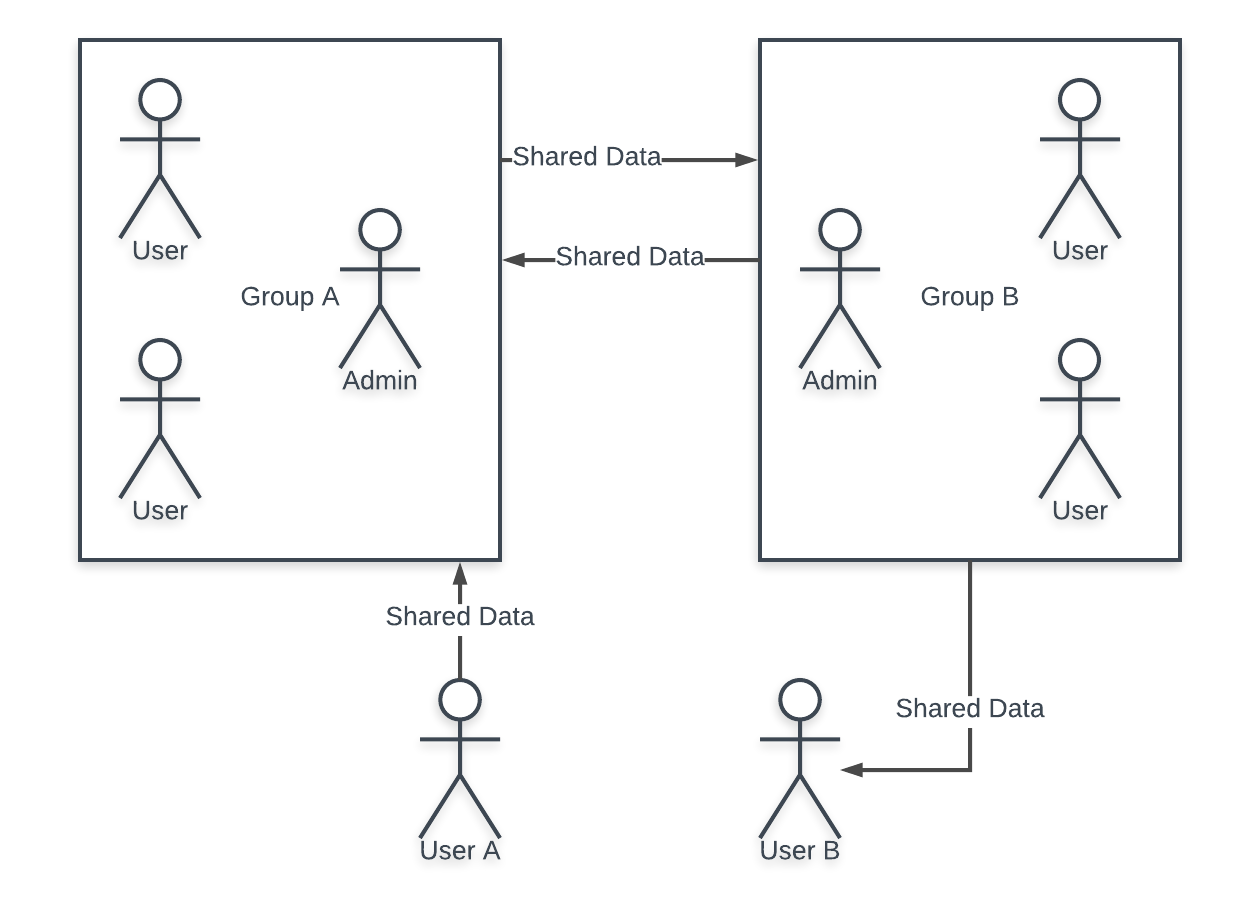
\includegraphics[width=0.8\linewidth]{DataPermissions}
  \caption{All users of Group A have permissions to User A\textquotesingle s data; All Users from Group A have access to the data of Group B and vice versa; User B Has rights to Group B\textquotesingle s Data; No group or user has access to User B\textquotesingle s data}
  \end{center}
\end{figure}

\subsubsection{Access Rights}
Users and groups may set two types of access rights to their files. The first being open and the second being restricted. As the name suggests, open files are open to the public. No special permission is required in order to access them. Thus, any user of our application may go to wherever they are hosted and pull them onto their own machine. If a user or group decides that they do not wish to have their files or data open to the world, then they may choose the restricted option. This option only allows certain users or groups to have access to the files or data. The specific rights are given as follows.\par
Users and groups may have different levels of permission given to them, refered to as access rights. These access rights can come in two forms: the right to read and the right to edit. The right to read allows a user or group to view the data the a user has published on the application and to download the files from the host machine onto their local machine. The right to edit allows users or groups to run analysis on data and use the tools we provide on the files or data. From that point forward, whatever the local user does with the data is beyond the control of either us or anyone affiliated with our program.

  \subsection{Testing}
\subsubsection{Guidelines}
Testing is an important part of any project. Traditionally tests are conducted manually via the developers themselves. Trying out different inputs and manually trying to break their code. While this method is tried and true for most computer science students, automated testing is needed to truly create a robust product. Automating our testing will maximizes the efficiency of our time. Allowing for more time to be focused on creating more features, rather than trying to break them. Especially with our product, since it focuses on a large amount data; ensuring that there are no bugs is a priority. The last thing we want is for a researcher to be weary of using our product in fear that he will achieve faulty results due to problems with the program. Creating a robust product with a high fault tolerance is on the forefront of our priorities.\par
Automation of testing can increase the resilience of a product but only if done correctly. Thus, a best practice of automated testing must be established. If these rules are followed then testing will be a blessing rather than a burden. The rules are as follows:

\paragraph{Not Everything Can be Automated} \mbox{}\\[\paragraphheaderspace]
Not everything can be automated, or rather, nothing can be automated easily enough to warrant its automation. As with any script, automating testing takes time. The more complex the test case, the more time it will take to develop a script that can successfully and efficiently ensure a program is working as expected. A good benchmark in deciding whether or not a test is worth automating is to determine how many times a task is repeated and seeing how similar each repeated task actually is. Tasks that are very similar and are repeated hundreds of times should be automated without a second thought. On the other hand, if a task is very variable and must be checked with more than a small set of test cases, then a human candidate might end up being better than a script. Some other things to consider when deciding whether or not to automate include:
\begin{itemize}
  \item \textit{Prone to human error} --- If a test is difficult for a human to construct then it may be better to write a script for it.
  \item \textit{Requires multiple sets} --- If a test requires a human to access multiple data sets across different platforms it may be easier to set up a script.
  \item \textit{High Risk} --- If a test is crucial to system performance, it may be a good idea to write a script that makes sure the section of code being tested works without a doubt.
\end{itemize}

\paragraph{Test Early and Test Often} \mbox{}\\[\paragraphheaderspace]
Ideally, testing should start as soon as the first section of code has been written. Unit tests can be conducted as soon as the first logical chunk as been made. Integration testing can be conducted as soon as more than a single section of the system is functional. Data testing can be conducted as soon as a full path for data is established. As soon as a type of test is feasible to be conducted, it should be done. This kind of mindset will ensure that most bugs are caught early and often. Not only will this make a more robust product, but it will save time in the long run of production. This results from the idea that, in most projects, it is usually the base off of which everything runs that is written first. If this is the case, then a bug created early on in a project will halt development for everything written on top of it.\par
Beyond testing as soon as possible, testing should be done every time a change is made to the way the code functions. This does not mean that every superficial change should be checked, since testing after trivial changes would be much too redundant and would slow down development. However, every time something significant changes in way in which the code functions, it should be tested. This will ensure that the vast majority of bugs will be discovered quickly, allowing us to pinpoint exactly where the bugs are happening and avoiding complex combinations of bugs to form.

\paragraph{Select the Right Automated Testing Tools} \mbox{}\\[\paragraphheaderspace]
Selecting the proper tools for a system is crucial in developing efficient solutions to automated testing. Without the proper tooling, creating an automated testing system can become an uphill battle that any development team could easily end up losing, rather than saving time. We considered the following when selecting our tools for testing the software:
\begin{itemize}
  \item \textit{The tool must support your platform} --- We decided to go with Spectron because it was specifically made to be used with our Electron front end. This will make it easier to test cases that will only occur in our Electron app.
  \item \textit{Simplicity in documentation} --- Our team consists of different levels of skill in terms of scripting. Thus, we decided to go with tools that are known to have good documentation. This way, those without as much experience in testing larger applications can learn quickly and start developing scripts for their sections of the code.
  \item \textit{Flexible Tests} --- When choosing a tool, we decided to go only with those that allowed us to make flexible tests. For example, Spectron scripts are not only resilient to changes in UI but can also be reused across multiple sections of the system
\end{itemize}

\paragraph{Create Good Test Data} \mbox{}\\[\paragraphheaderspace]
Data for test cases should cover all kinds of possibilities for the code being tested, preferably in the most efficient way possible. Rather than create an extensive list of all possible inputs, it\textquotesingle s best to create sets of data that test all edge cases, as well as any other special cases that may cause problems with the code. Along with constructing good test data, it can be useful to construct external file sheets. By using external file sheets, we will be able to reuse test scripts over several sections of similar code. This is because, as opposed to hard coded data, having external data allows us to easily change what is being input to our scripts, allowing us to quickly create new test cases with appropriate data.\par
We will also be using a mixture of auto-generated and specially constructed data. The auto-generated data will be used when a vast set of data is needed to test the functionality of a code section. Data files provided to us by our sponsor will be used when specific data sets are needed. This will make sure we have a good mixture of random data and real world data to test our product.

\paragraph{Make Robust Testing Scripts} \mbox{}\\[\paragraphheaderspace]
When creating our scripts, we will use configuration files. Doing so will allow us to reuse our scripts through multiple design iterations. These configuration files will contain variables within the code. These variables will be variable names, positions of elements in the UI, and any other dynamic elements that we think will need to be changed.

\subsubsection{Methodologies}
There are several testing methodologies available to us. We will use a combination of several types of testing in order to ensure our entire system is fool-proof. The following four testing types will be used:

\paragraph{Unit Testing} \mbox{}\\[\paragraphheaderspace]
Unit testing involves testing the smallest piece of code that can be logically isolated from a system. This piece of code can be a function, a subroutine, or a method. This type of testing should be conducted by the programmer. This is due to the fact that unit testing should be done continuously while developing a section of code. Making it most efficient when implemented by the programmer. We will be unit testing functions and API calls that are made before adding them to the main code. This will ensure that the number of faulty methods that are introduced are minimal.\par
The reason unit testing works so well stems from the idea that a whole is just made up of smaller parts. If each of the smaller parts of a system are working then in theory the whole system should work. In practice other types of tests are needed to ensure all subsystems are working together properly, but unit testing does resolve many of the issues within the subsystems. Resolving local issues makes it much easier to debug the whole system during the final stretch of the project.

\paragraph{Integration Testing} \mbox{}\\[\paragraphheaderspace]
Integration testing involves making sure that the connections between pieces of a system are working properly. This is the area in which unit testing tends to miss bugs and where most bugs are actually found. The reason for this is that unit tests should only be used on small logically separated pieces of code. So, when different sections are joined together, the undiscovered bugs come out. Additionally, different sections are usually programmed by different developers, meaning that there may be conflicts due to unexpected outputs or unexpressed requirements for each section. This is where integration testing comes in. In order to properly perform integration testing, it becomes necessary to take a step back from the code and analyze the flow of data through the system. This allows for any logical errors to be sniffed out before running tests. After making sure that the flow of data is working as expected, it becomes possible to run automated tests that send data all the way through the system. This makes sure that all points of connection are working properly and that data is not being corrupted or changed erroneously.\par
Without integration testing at every connection point, debugging code can become very difficult. This is due to the possibility of data ``black holes,'' where data is either corrupted or completely lost somewhere in the pipeline of the system. If a system is fully built without testing each connection point, it can be almost impossible to pinpoint exactly where a black hole is happening. Therefore, our team will conduct integration tests at every connection between any two software units.

\paragraph{Functional and Data-Driven Testing} \mbox{}\\[\paragraphheaderspace]
While functional testing and data-driven testing are separate ways of performing automated testing, in our project, they will be conducted in almost an identical manner. Once the project has been built to a functional point. We will assume the role of users and gauge the experience when using the product. This is the methodology of functional testing. While usually implemented by a team of individuals, for our product, much of the experience lies in how the data is processed and displayed. This is where data-driven testing comes into play. We will pass multiple sound files and see if they match their expected outputs. If the outputs match we will then analyze the runtime and determine the clarity of the charts. This method of combining both functional testing and data-driven testing will allow us to fully view the functionality of our product from the perspective of a user.\par
During the data-driven portion of testing we will also be introducing some chaos testing to the mix. This involves running the product in several different environments, i.e. Mac, Linux and Windows. Within each of these separate environments we will also run a number of common applications a user might be running alongside our program. This will simulate real world use, allowing us to see how our product performs with, for example, fluctuating CPU and RAM usage. It will also allow us to see whether or not there are any compatibility issues with other programs which, while rare, can be detrimental to our product. Another element of chaos testing we will implement will be random shut offs and disconnections from networks during processing. This will ensure that no data is corrupted or permanently lost during these emergency events. Performing this type of testing will allow us to see that our product is robust and secure, even during complete failures of the system that is running it.

\subsubsection{Frameworks}
We will use a combination of frameworks in order to test our product. These frameworks include Chai, Mocha, and Spectron. Each of these frameworks is tried and true, known well in the JavaScript development community for their ease of use in testing in Node.js environments.

\paragraph{Chai} \mbox{}\\[\paragraphheaderspace]
Chai is an assertion library purposed for behavior-driven and test-driven development in Node.js. We will use Chai as Promised, which extends Chai, for asserting facts about JavaScript promises. Thereby, we can transform any Chai assertion into one that acts on a promise. Combining Chai with Spectron will provide a powerful tool that allows us to use JavaScript promises.

\paragraph{Mocha} \mbox{}\\[\paragraphheaderspace]
Mocha is a feature-rich JavaScript test framework running on Node.js and in the browser. Mocha tests run serially, allowing for flexible and accurate reporting, while mapping uncaught exceptions to the correct test cases. Mocha allows us to use Chai as our assertion library. It also supports asynchronous testing, which can be useful when running tests with large amounts of data inputs.

\paragraph{Spectron} \mbox{}\\[\paragraphheaderspace]
Spectron is an open source framework for writing automated tests for Electron apps. It allows developers to navigate web pages, simulate user input and run dedicated tests. It also simplifies the use of other testing frameworks by making the setting up, running, and tearing down of Electron environments easier. Developed by GitHub, it is the dedicated testing framework for Electron, and therefore, it is the first choice for writing test cases for our Electron-based front end application.\par
The following example code finds the application, checks to see if there is a visible window containing the title \lq My App\rq, and finishes by logging any errors:

\begin{javascriptcode}
// A simple test to verify a visible window is opened with a title
var Application = require('spectron').Application
var assert = require('assert')

var app = new Application({
  path: '/Applications/MyApp.app/Contents/MacOS/MyApp'
})

app.start().then(function () {
  // Check if the window is visible
  return app.browserWindow.isVisible()
}).then(function (isVisible) {
  // Verify the window is visible
  assert.equal(isVisible, true)
}).then(function () {
  // Get the window's title
  return app.client.getTitle()
}).then(function (title) {
  // Verify the window's title
  assert.equal(title, 'My App')
}).then(function () {
  // Stop the application
  return app.stop()
}).catch(function (error) {
  // Log any failures
  console.error('Test failed', error.message)
})
\end{javascriptcode}


  \subsection{Facilities \& Equipment}
\subsubsection{Equipment}
\textbf{QNAP}\\
Our sponsor has access to a device called a QNAP. A QNAP acts as a local storage device but also as a remote server when needed. This device is useful for our project because it gives us access to a sort of private server option for our users, if they would prefer not to use a OneDrive service or something similar. In using a QNAP or other private device, the users can specify files and folders for others to access and provide those access rights to our service for others to use. The QNAP is also handy because it provides a built in interface for users to tap into and easily find the files being offered by the provider.\\\\
\textbf{Microphones}\\
Some important equipment used by the researchers in the field of soundscape ecology include microphones. Our sponsor in particular uses a Wildlife Acoustics SM4 model along with the Wildlife Acoustics Song Meter device.\par
The Song Meter is considered the smallest and lightest dual channel acoustic recorder available\cite{songmeter}. The microphones record raw sound and store them in uncompressed .wav files. These .wav files can then be used by programs like ours to calculate the indices mentioned for analysis by researchers.\par
Our sponsor\textquotesingle s strategy is to place these microphones in multiple places in the environment being tested, to get a better understanding of the impact of sound on the ecosystem. In doing this, we can hear more of the sounds of the ecosystem and provide better index analysis.\par

\subsubsection{Facilities}
\textbf{UCF Arboretum}\\
The UCF arboretum was created in 1983 as a place for students and faculty to learn about ecology and work with the environment. The arboretum acts as a research area on campus for identifying plants and the local wildlife\cite{ucfarboretum}. This eighty acre span of land is home to hundreds of species of plants and animals, including vulnerable species like the Gopher Tortoise.\cite{pegasus}\par
Over the past year, our sponsor, Dr. Beever, has been conducting research in the arboretum and surrounding areas to gain a better understanding of the impact of humans on the local ecosystem using the Wildlife Acosutic microphones. One interesting segment of this research is a series of recordings made of Hurricane Irma during the 2017 hurricane season. With sustained wind speeds in the Orlando area during this hurricane reaching 59 mph (95 km/h),\cite{irmaspeed} the potential insights found from possible biophony within the recordings may prove to be intriguing.\\\\
\textbf{Central Florida Zoo}\\
Originally founded as the Sanford Zoo in 1923, the Central Florida Zoo has since become host to over 400 animals. It has since adopted a mission which, among other tenets, includes ``contributing globally to the conservation and preservation of wildlife.''\cite{aboutzoo}\par
\begin{center}
	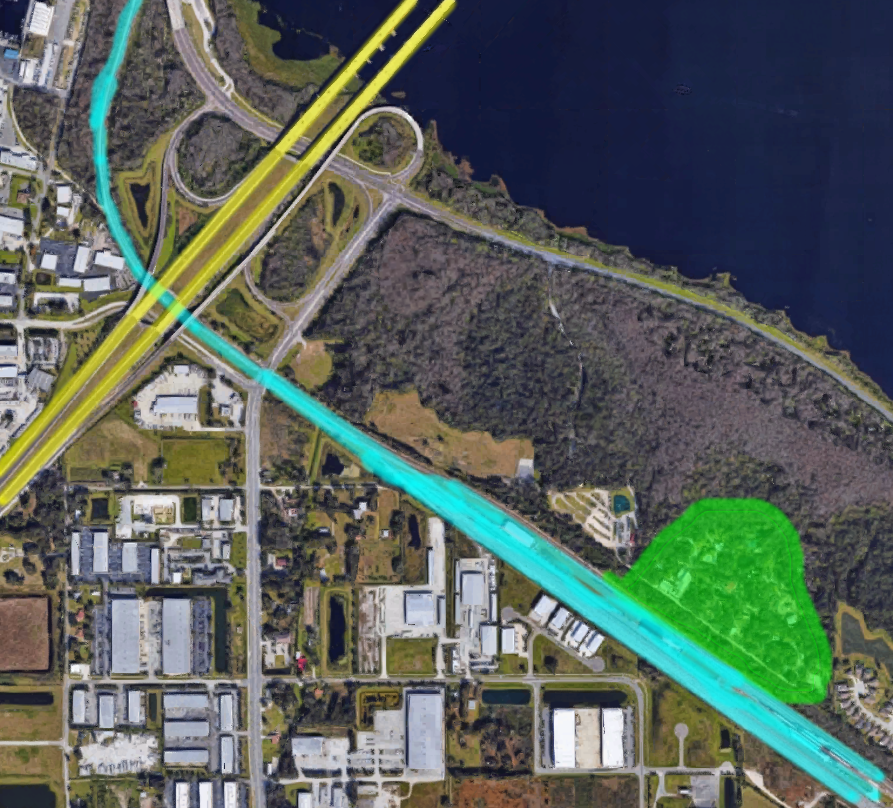
\includegraphics[width=\textwidth]{ZooMap}
\end{center}
In the past year, Dr. Beever obtained permission from the zoo (green) to place several of his microphones within the giraffe enclosure. With the enclosure only steps away from a Class I railway (blue) and about a mile away from Interstate 4 (yellow), he was curious to see how these massive sources of anthrophony could affect the biophony produced by the giraffes and, consequently, their general well being.

  \subsection{Machine Learning}
The field of soundscape ecology has made astounding progress in the last decade.
Recordings and new techniques have allowed for the gathering of massive amounts of sound data. While this remains good news for the field, it raises new problems. Who or what will listen to these recordings, and how can they be analyzed in an efficient way? Many techniques have cropped up, most prominent of which is having hired experts listen to recordings, but the technique we are focused on in this project are the use of indices. These indices are algorithms that can be run on sound files, which then produce numerical values that can uncover generalizations about the sound (more information be found in the Soundscape Ecology Indices section).\par
While the soundscape ecology indices have great potential, they have not yet been rigorously tested and are currently in the process of being tried out in field studies. The main downfall of the indices is that they are used to compress vast amounts of data about the health of an environment into relatively few data points. This leads to a loss of information. Along with this lossy compression, sound files must also be cleaned before the indices can be properly used. The cleaning often involves chopping off certain frequency ranges or manually removing geophonic and anthrophonic sounds in the recording. This cleaning, combined with the already lossy nature of the indices, provides very rough numerical descriptions of the sound files, which have yet to be proven completely accurate in general circumstances.\par
Due to the nature of the indices, they are often used alongside another method to verify their accuracy. As mentioned previously, experts are often used, and this method is often costly and time-consuming.\par
In researching machine listening, our goal was to determine the best techniques and models that could be used to recognize species\textquotesingle\ sounds. While the methods listed in the following sections are quite robust, in the sense that they have high accuracy ratings when used, they cannot be used for general cases. Depending on the machine learning methodology, it may or may not become necessary to build a unique model for each species of bird, and this makes it less than ideal as a substitute for the indices, but an ideal technique for verifying the indices\textquotesingle\ results in a specific environment. We hope that future groups may take advantage of our research and put it to use in furthering the Mangrove application.\par
\begin{center}
	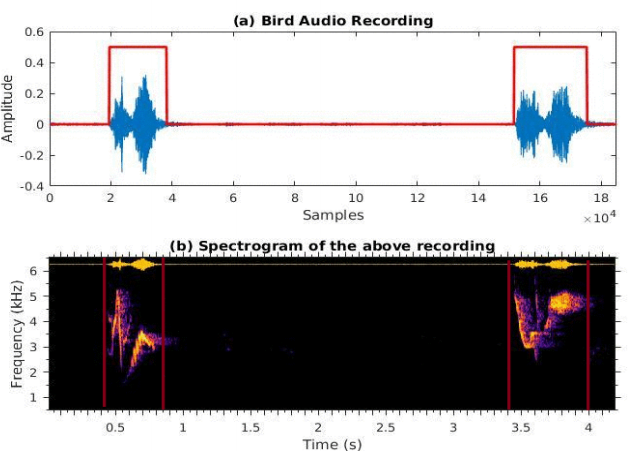
\includegraphics[width=.8\textwidth]{bird_spec}
\end{center}

\subsubsection{Bayesian Networks}
In this project we will use a modified version of Hidden Markov Models in order to recognize bird calls and possibly other animal sounds. This complicated system starts off with a very fundamental fact of life. ``All models are wrong, but some are useful,'' meaning that getting an exact representation of the real world is impossible. Either some assumptions are incorrect or the way we represent the world leaves out some information. However, while some information will always be left out of a model, it is still possible to construct one that is useful.\par

\begin{center}
  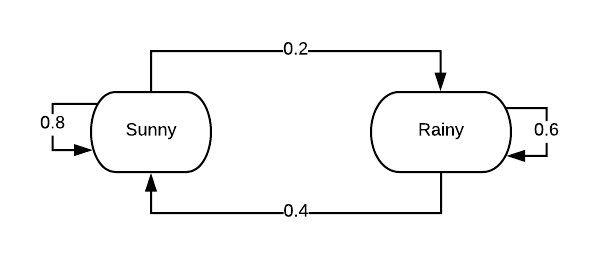
\includegraphics[width=.8\textwidth]{basicmodel}
\end{center}

The models we will be constructing are called probabilistic models. The very bases of these models are that the chance of moving from one state to another can be found out using previous data. After extrapolation, a model of state space and chance of movement between these states can be built. Using the model above as an example, we can see that we have two states: Sunny and Rainy. The chance of either staying in a state or moving from one state to another can be seen by looking at the arrows. The probability of moving is shown as a number from 0 to 1 (0\% to 100\%). While this is not a Bayesian network, it is the very basic idea from which Bayesian networks are built. Using the above model, we can create a conditional probability table (CPT). The corresponding table can be seen below.\par

\begin{center}
	\begin{tabular}{|c|c|c|}
    \hline
		\tablehead{Current}
    & \tablehead{Next}
    & \tablehead{Chance}
    \\ \hline

		Sunny
    & Sunny
    & 0.80
    \\ \hline

		Sunny
    & Rainy
    & 0.20
    \\ \hline

		Rainy
    & Sunny
    & 0.40
    \\ \hline

		Rainy
    & Rainy
    & 0.60
    \\ \hline
	\end{tabular}
\end{center}

Now that we have some idea of what a probabilistic model is, we can apply one of the most useful concepts in Bayesian networks: \textit{conditional independence}. This means that one variable is independent from another variable, depending on given information. The formula for calculating conditional independence is as follows:\par

\begin{equation}
  \textnormal{Independence: }
  P(A|B) = P(A)
\end{equation}
\begin{equation}
  \textnormal{Conditional Independence: }
  P(A|B,C) = P(A|C)
\end{equation}

An example of this would be if you have an alarm system. Every time there is a break-in at your house, there is a high chance that the alarm goes off. When the alarm goes off, there is also a chance that your neighbor calls you. Initially with no information, your neighbor calling you will be dependent on whether or not there is a break-in. This changes when you know that the alarm is already ringing. The reasoning for this is that if you already know the alarm is going off, knowing that there is a break in does not give you any more information on the alarm going off. Since the alarm is the only thing that can directly affect your neighbor calling you, then the break-in variable is conditionally unlinked from your neighbor calling you, making the two variables independent.\par
It is possible to map out interactions like this with a Bayesian network, each node being a variable and each arrow connecting two dependent variables. These networks must be acyclic directed graphs. The following figure demonstrates the previous example with added variables: earthquake and one additional neighbor. The alarm is dependent on the earthquake and your other neighbor calling is still dependent only on the alarm.\par

\begin{center}
  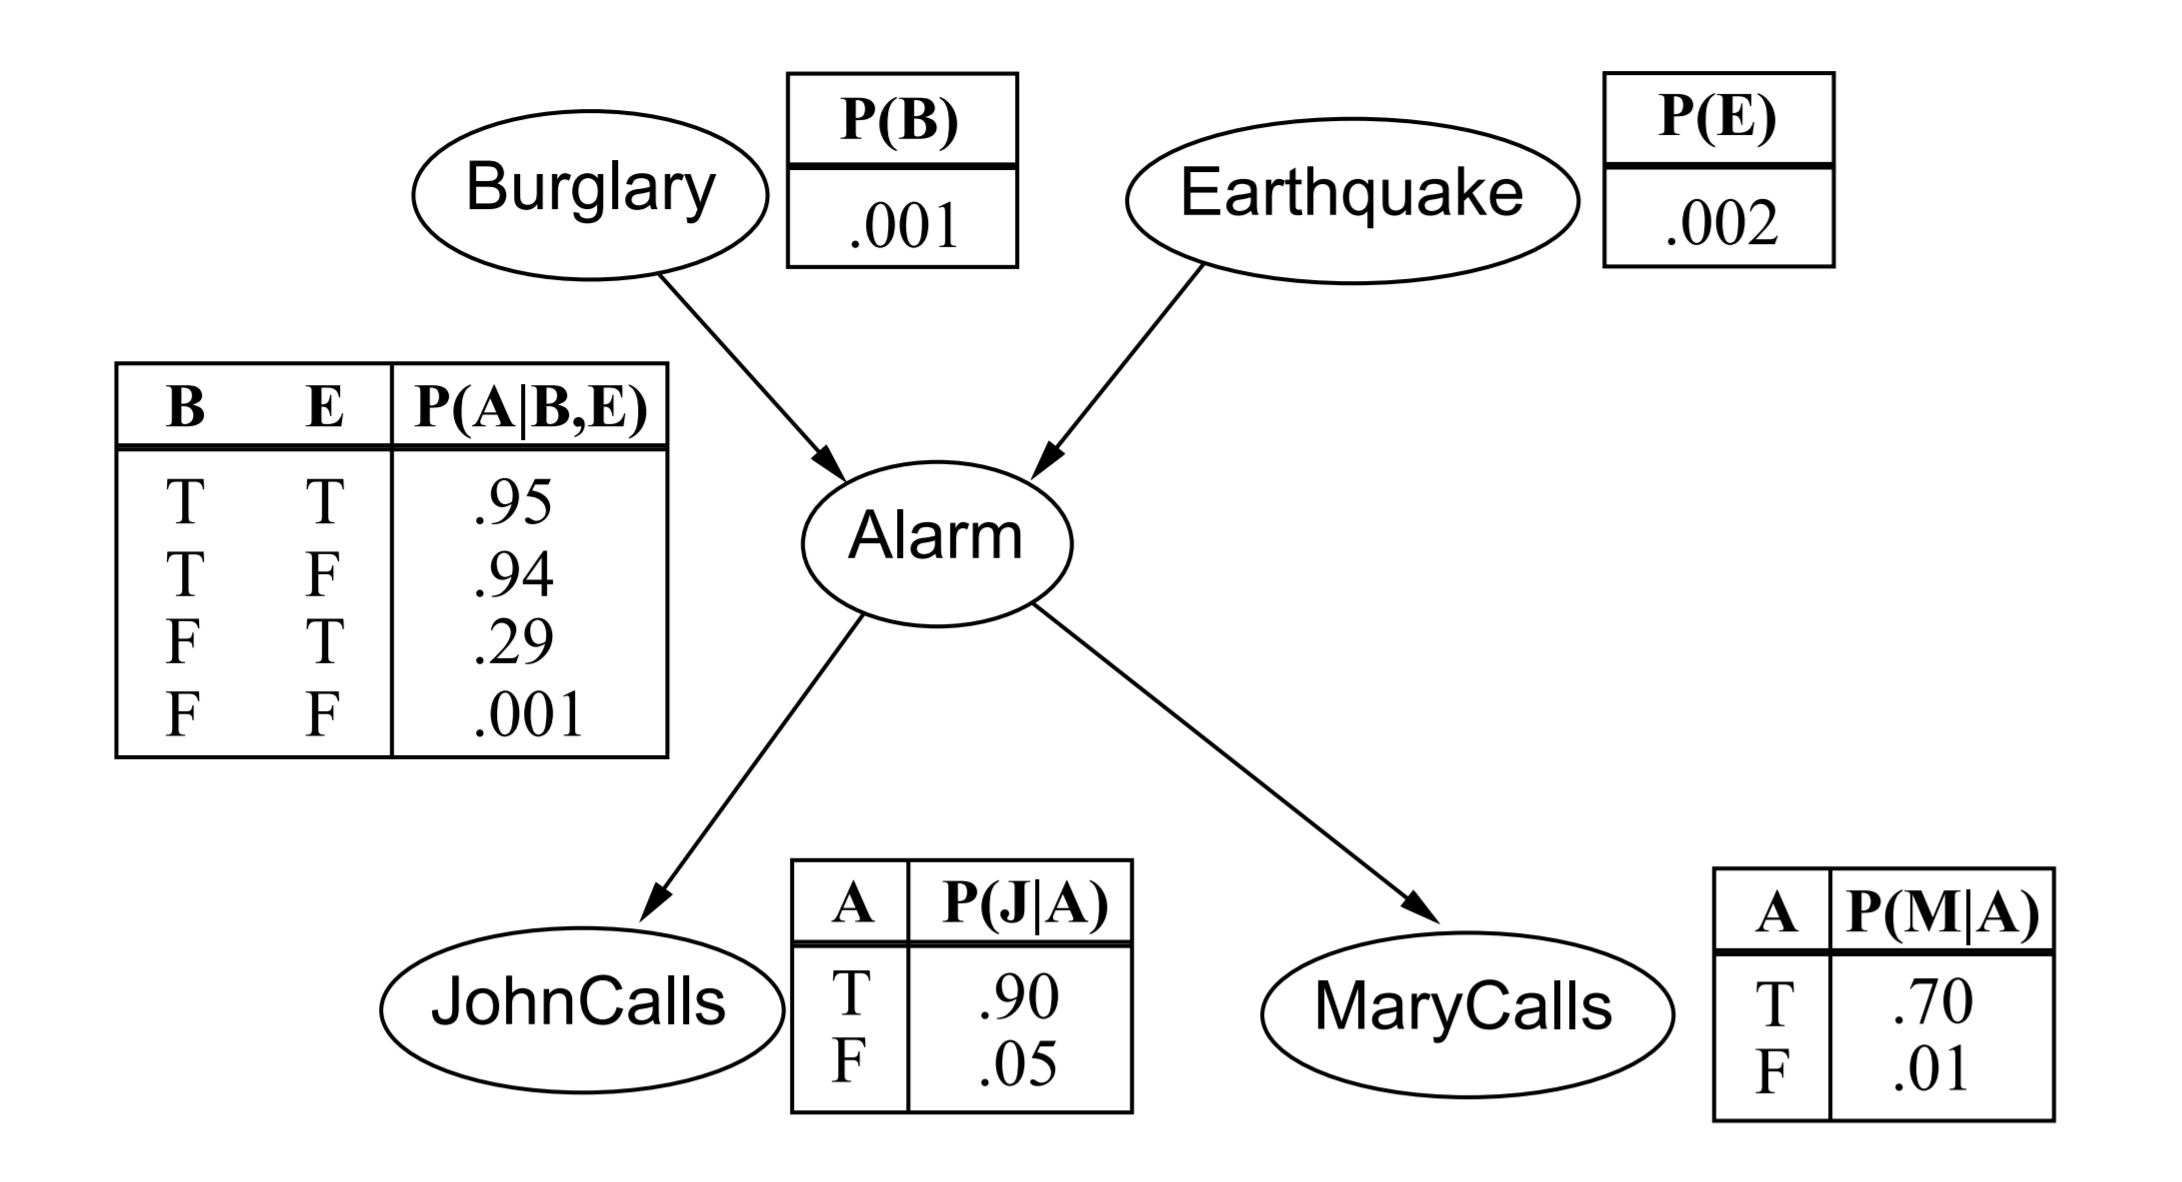
\includegraphics[width=\textwidth]{bayesnet}
\end{center}

With graphs like these, it becomes easier to identify the conditionally independent variables and reduce the size of our corresponding CPT\textquotesingle s. This vastly improves the speed of calculations, since CPT tables grow on a factor of $2^N$ where $N$ is the number of dependent variables. For example, if conditional independence was not used in the figure above, the CPT for JohnCalls would contain 8 (via $2^3$) entries. This is reduced to just 2 entries since Burglary and Earthquake become independent once Alarm is known.

\subsubsection{Markov Models}
Markov models can be considered chain structured Baye's Nets. Where each network is tied into the previous and next network in a fashion similar to a linked list. We can consider each network a node along that linked list. Each node within this "list" contains the same CPT, excluding the starting node. The very first node has a CPT that represents the initial probability distribution of the starting state. Since these node are Baye's Nets similar classes of problems can be modeled. The advantage is that with the addition of linking an element of time can be added. Taking this into account we can see why the CPT for each node after the initial node is the same. It takes into account the probability of state space changes from one state to another. In technical terms we can call this a transition model and it can be described by the following equation:
\vspace{10px}
\begin{center}
$P(X_{t+1}|X_{t})\:$Where $X_{1}$ is the initial state.
\end{center}
\vspace{10px}
This basic idea can be implemented over, theoretically, infinite time steps. Where at each time step you apply the transition function onto the Baye's Network. The function is as follows:
\vspace{10px}
\begin{center}
	$$\sum_{X_{t-1}} P(X_{t}|X_{t-1})\:P(X_{t-1})$$ where $X_{t-1}$ is the previous time step.
\end{center}
\vspace{10px}
This type of algorithm goes by the name Mini-Forward Algorithm. A very interesting quality of this algorithm is that for infinite time steps you most always reach a convergent state. Meaning that the $X_{t-1}$ time step will be equal to $X_{t}$ for all following iterations. This property allows us to find a final resting state within a stochastic system. Which can be useful for many applications.
--Include how this relates to vocal recognition.
\subsubsection{Hidden Markov Model}
While Markov Models are very descriptive models of an environment, oftentimes when analyzing sound data, we do not have the information to paint the full picture. This means that we don\textquotesingle t have the full sequence of states, but we do have measurements from those states. Specifically, our states are the specific sounds that are made by an animal. We can call this a syllable (many bird songs consist of syllables). Unfortunately, we do not know these syllables, we only know the acoustic signals that they produce. These signals would be the evidence or observation in our current definition of the Hidden Markov Model (HMM). Using the sound waves we translated via Fourier transform, we can eventually get to the actual syllables made by the animal.\par

\begin{center}
  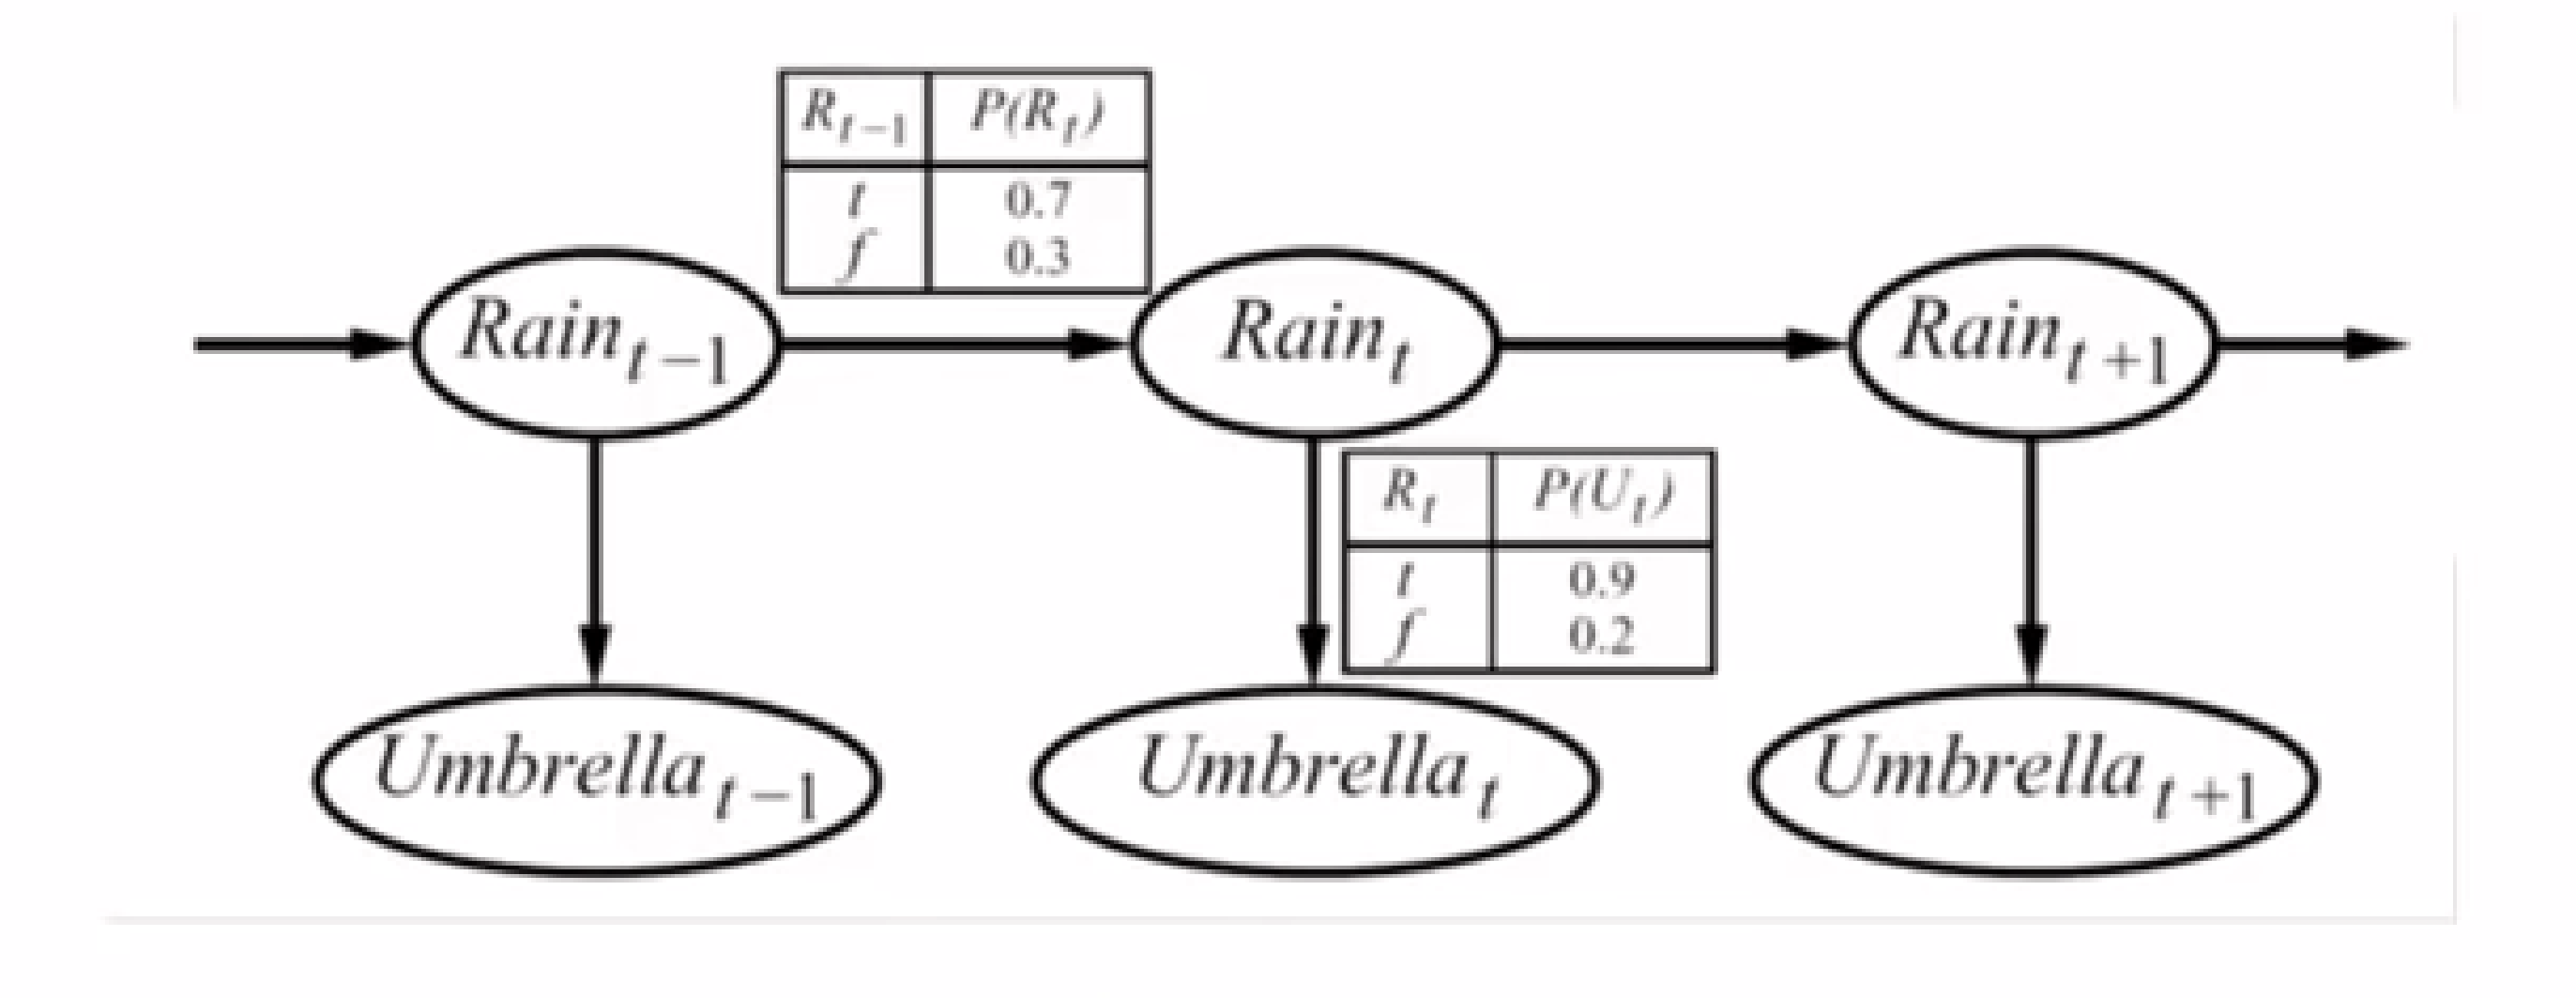
\includegraphics[width=\textwidth]{HMM}
\end{center}

When we talk about HMM, we are talking about the belief the current system is in. This is in reference to running an inference of the state based on what kind on evidence we have received. An example would be figuring that there is a 60\% chance that, with the current configuration of sound waves, syllable A is the sound made by the bird. This belief is obtained by filtering the current state with previous evidence. The method can be described by the following:\par

\vspace{-32px}
\begin{center}
  \begin{equation}
    B_{t}(X)
    = P_{t}(X_{t} | e_{1}, ..., e_{t})
  \end{equation}
  where e is the evidence and X is the current state.
\end{center}

We then update the belief via the following function:\par

\vspace{-32px}
\begin{center}
  \begin{equation}
    B'(X_{t+1})
    = P(X_{t+1} | e_{1}, ..., e_{t})
    = \sum_{X_{t}} P(X_{t+1} | X_{t}) P(X_{t} | e_{1}, ..., e_{t})
  \end{equation}
\end{center}

We must then re-weight the likelihood of the current belief based on the probability of that belief state with the current evidence, using:

\vspace{-32px}
\begin{center}
  \begin{equation}
    B'(X_{t+1}) P(e_{t+1} | X_{t+1})
  \end{equation}
\end{center}

The following image shows how HMM\textquotesingle s update their belief based off of time updates and then evidence updates.

\begin{center}
  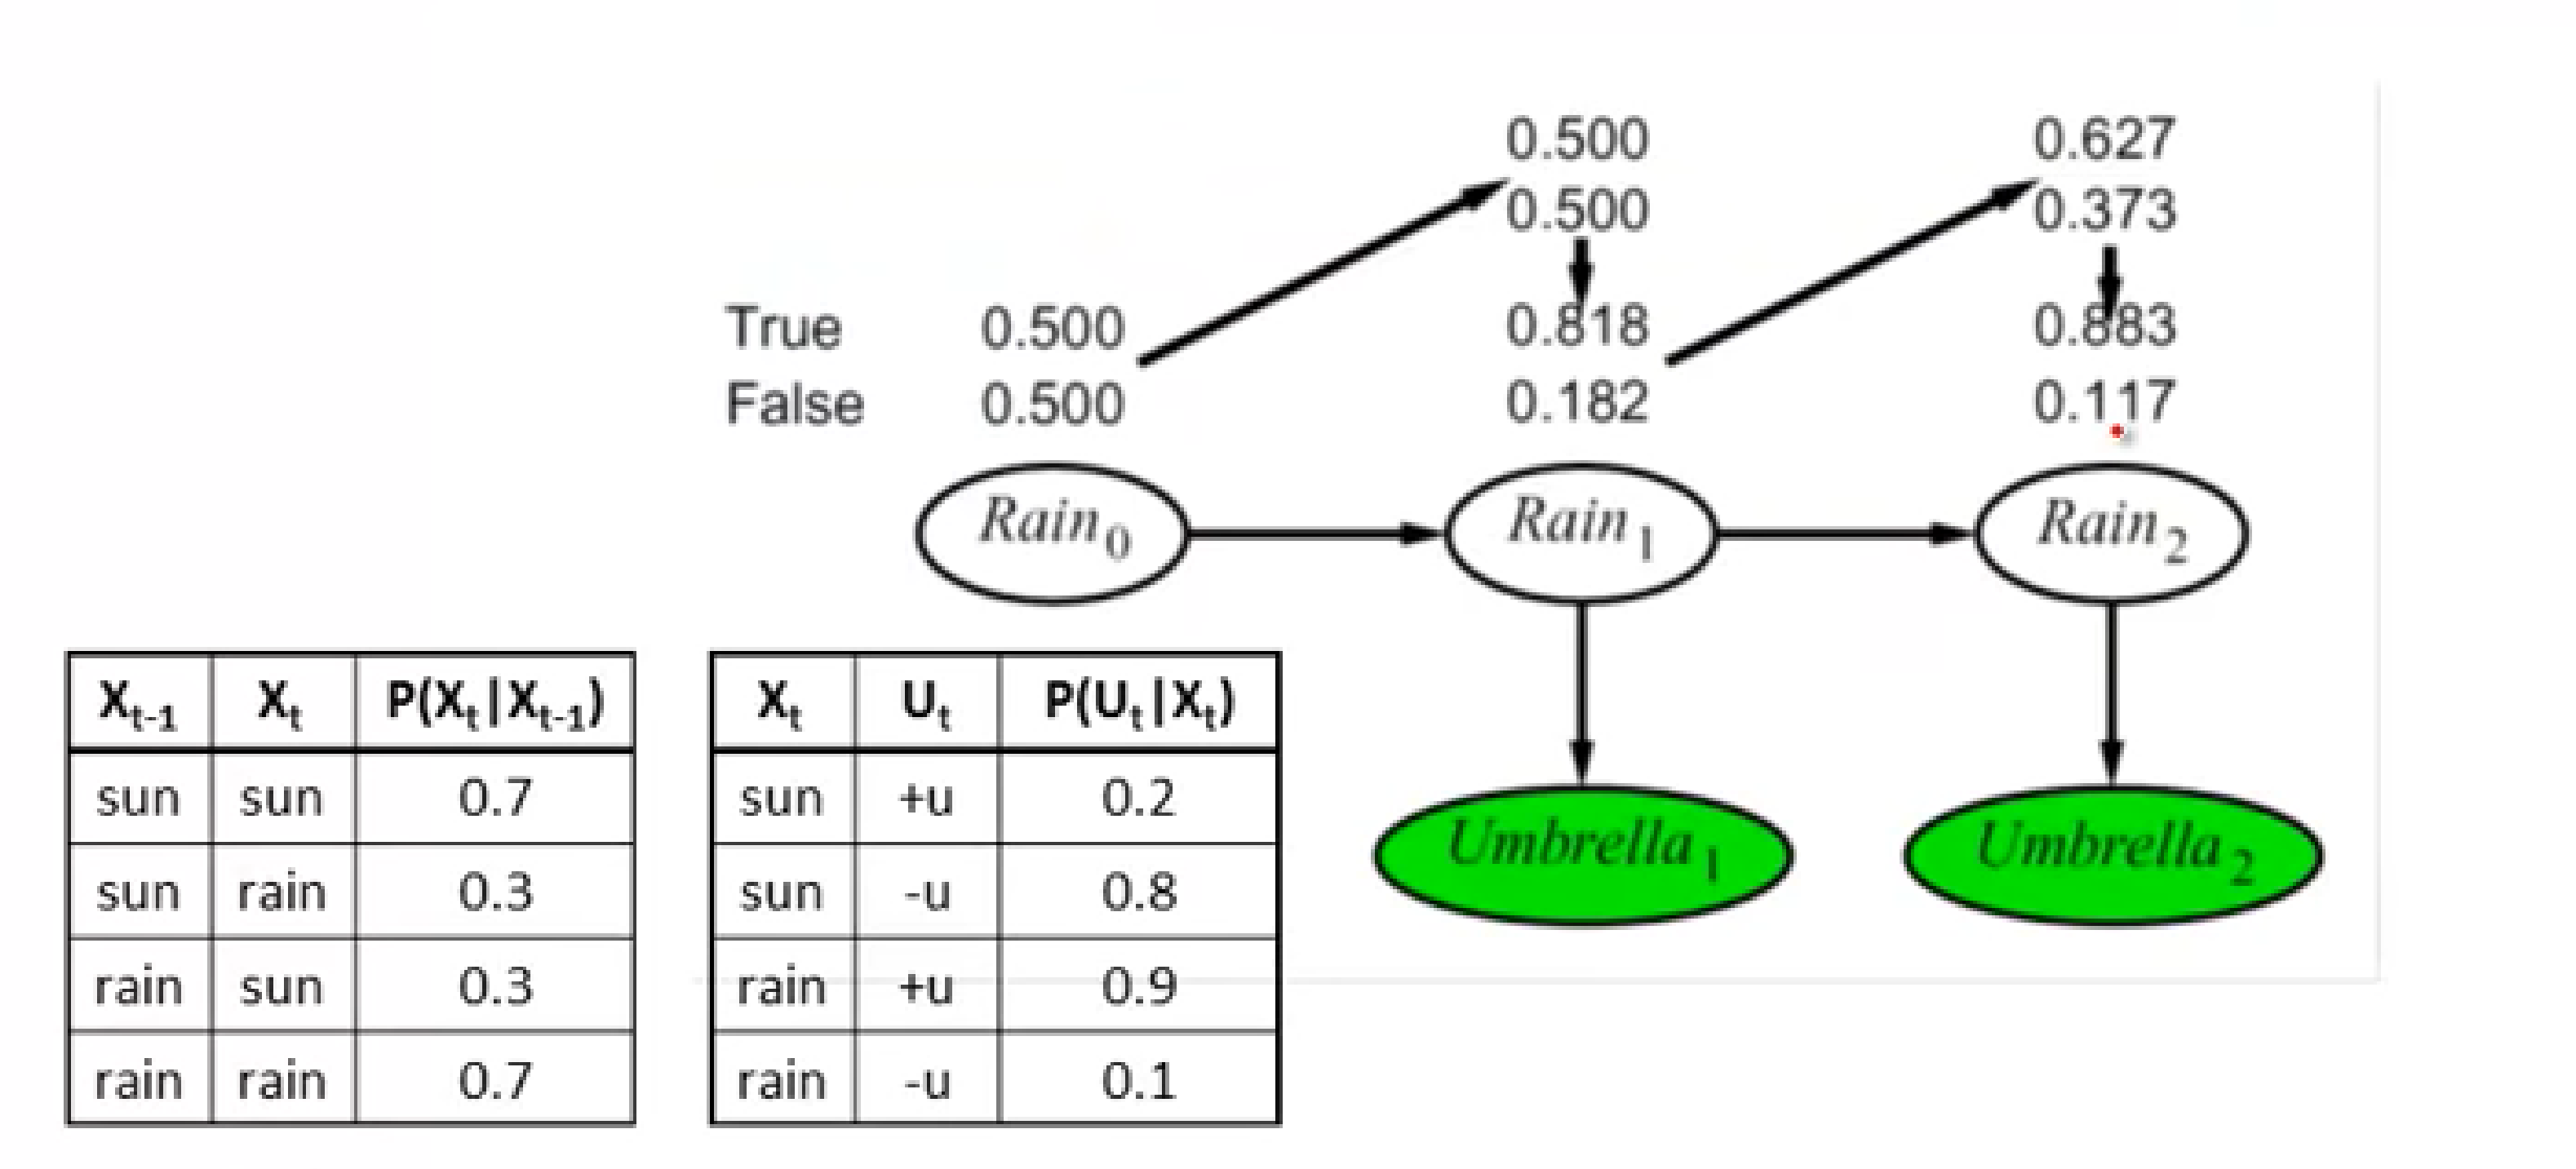
\includegraphics[width=\textwidth]{HMMupdate}
\end{center}

\subsubsection{Speech Recognition}
\par Most speech patterns can be broken down into basic parts. We know these familiar parts as syllables of speech. These discrete sections of words can be combined together to form long strings of sentences. For our case these sentences are the songs of the birds. Syllables are made using a basal tone in the throat of the animal, which is then filtered by a formation of the muscles around the throat.
Due to this, many syllables have repetitive sound structures that, when transformed by the Fourier transform, can be modeled by HMM.
\begin{center}
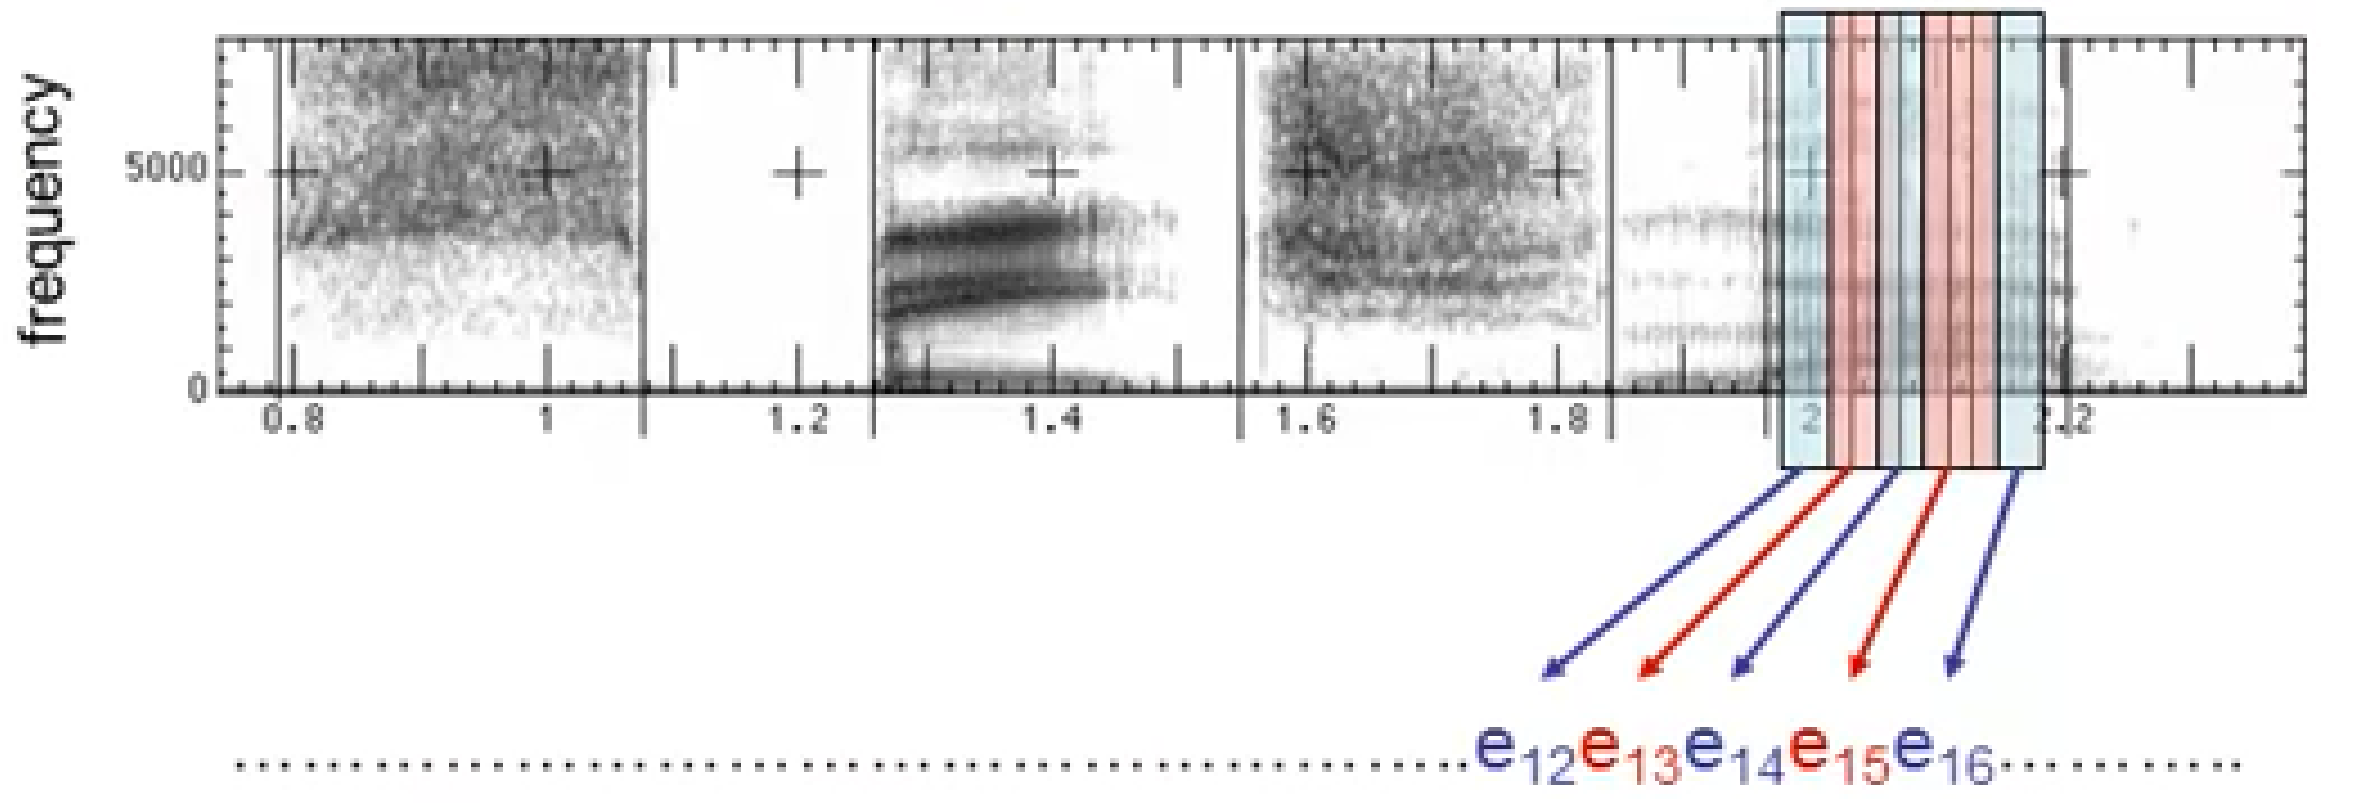
\includegraphics[width=\textwidth]{HMMSpeech}
\end{center}
\par For each slice of the spectrograph that we analyze the actual sound that was emitted and transformed is the evidence. Since it is directly dependent on what syllable is being said. That same syllable is our hidden state. The state space for these states consists of all the syllables that a bird species can produce. It is easy to see why expanding this to a system that included several different types of animals would increase the state space far too much to have efficient analyses of the sounds. 
\par As shown in the model below the when you enter a state space that represents the syllable you have a probability of staying within that state space. This probability decreases as time continues as the likelihood the syllable is still being held goes down. While within this state space evidence is produced based on a probability model used for the specific syllable you are in. Once the probability is low enough it becomes likely that you syllable will move to another state space.
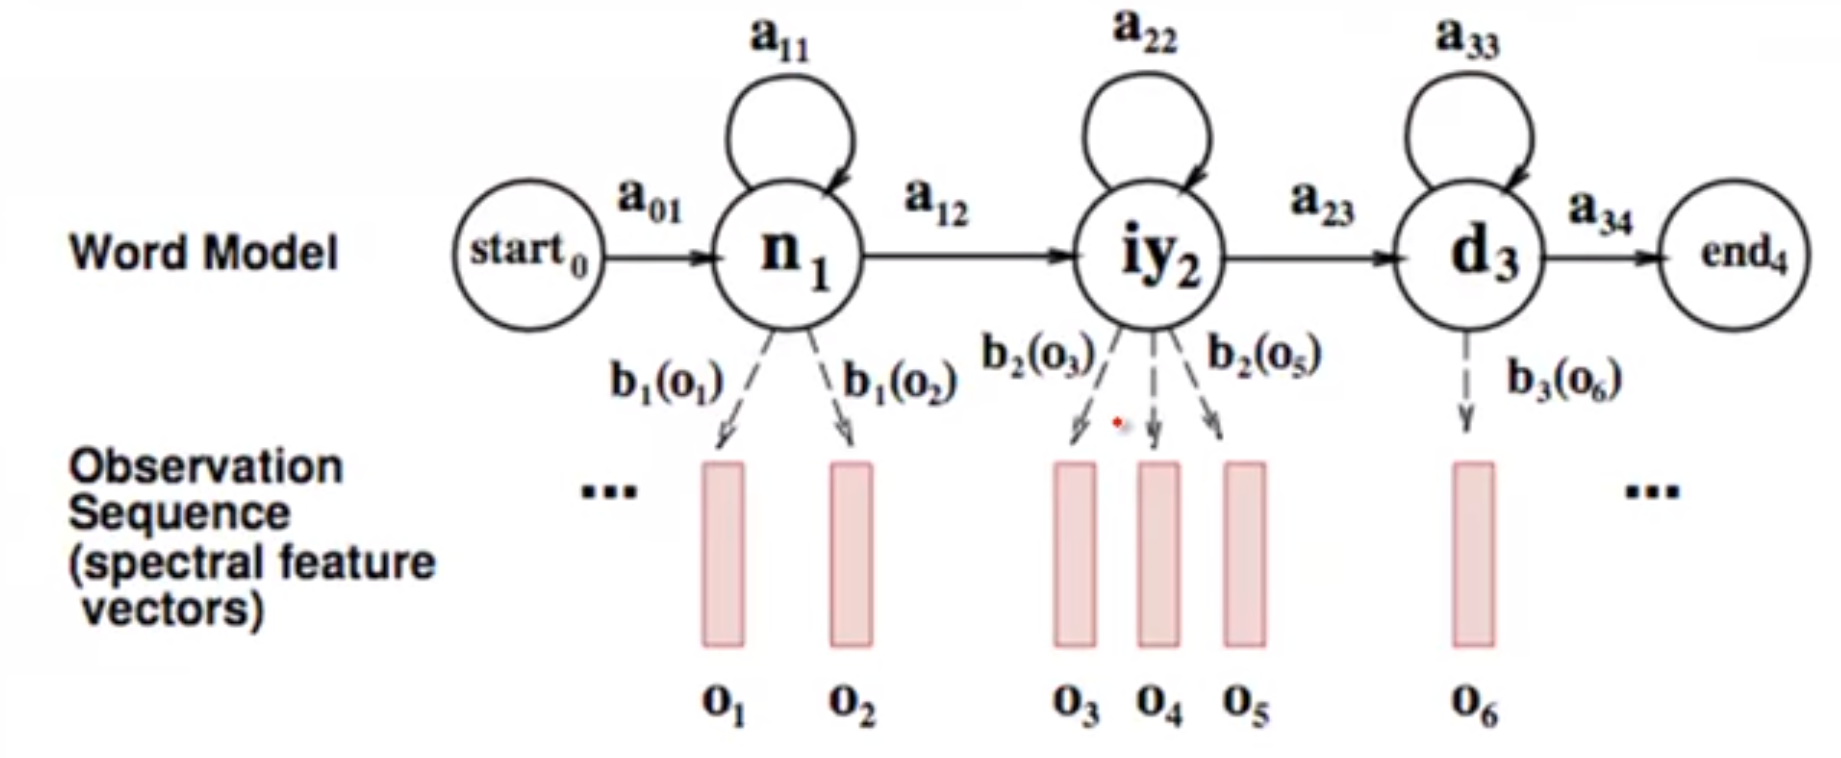
\includegraphics[width=\textwidth]{transitionModel}
Something further to consider would be the use of a bigram model. This model uses groupings of bird song syllables to construct "words". This would allow the positioning of these words to give information on upcoming words. Much like in human languages the use of certain words increases the chance of upcoming words. Models like these would further improve the accuracy of our analysis.  





  \subsection{Benchmarking}
The process of analyzing the sound files in the field of soundscape ecology is quite painful as it stands. Currently, our sponsor uses wav format sound files of size 1.29GB, each a recording of ten minutes long. Some datasets used include over one hundred sound files, which amounts to over 100GB of sound files to process. It is important to know the length of time needed to process these files locally based on the end user\textquotesingle s hardware. The following are the results of NDSI index analysis on a single sound file of size 1.29GB, and the respective hardware involved. As a side note, it seems important to add that in order to run analysis on sound files in R, each wav file must be converted to a Wave object in R to be used in the index processes. This alone has proven to be a lengthy process on lower end systems.\\

\noindent\textbf{Intel i5 6500 @ 3.2GHz / 16GB RAM}\\
The analysis took 686.64 seconds to process a single 1.29GB wav sound file. That comes out to 1.29GB in eleven minutes and forty four seconds. For a data set comprised of one hundred 1.29GB sound files, that would estimate to around nineteen hours for 129GB of sound files.\\

\noindent\textbf{Intel i7 7500U @ 2.7GHz / 16GB RAM}\\
The analysis took 1045.95 seconds to process a single 1.29GB wav sound file. That comes out to 1.29GB in seventeen minutes and twenty five seconds. For a data set comprised of one hundred 1.29GB sound files, that would estimate to around twenty nine hours for 129GB of sound files.

\noindent\textbf{Intel i5 5200U @ 2.2GHz / 8GB RAM}\\
The process of converting this single wav file to a Wave object in R actually managed to freeze this system for around 30 minutes, before any analysis even began. Then after 315.4 seconds, a little over five minutes, the processing stopped with an error reading "cannot allocate vector of size 1.3GB." This was an unexpected result, raising questions as to possible user minimum required hardware specs. Thus, with this hardware, processing is not even feasible.\\

\noindent\textbf{Intel i7 6500U @ 3.1GHz / 24GB RAM}\\
The analysis took 585.19 seconds to process a single 1.29GB wav sound file. That comes out to 1.29GB in nine minutes and forty five seconds. For a data set comprised of one hundred 1.29GB sound files, that would estimate to around sixteen hours for 129GB of sound files.


\noindent\textbf{Conclusions}

  \newpage

  \section{Administration}
  \subsection{Plans for Successful Completion of the Project}
In order to achieve the timely completion of our project, a series of principles have been established amongst ourselves. Many of which were inspired by the Senior Design Bootcamp in August.
\begin{itemize}
  \item \textbf{Frequent collaboration/meetings:} By agreeing to meet twice a week, our team members have the opportunity to raise concerns and ensure accountability with each other. And in addition to collaborating in person, we use technologies such as Github, Discord, and Google Drive to keep ourselves in the loop.
  \item \textbf{Setting Goals:} For each meeting, an agenda is written and followed to ensure that all necessary topics are addressed. This includes meetings with TAs and our sponsor, Dr. Beever.
  \item \textbf{Understanding Values:} For each person involved in this project, their exact definitions of success and quality will differ from those of others. Thus, through greater understanding of  our motivations, our ultimate goal should be easier to achieve.
  \item \textbf{``Creating 100 Ideas:''} This concept of continuously questioning the current solution was described during the Bootcamp. By creating ``100 ideas'' our team could gain a better idea of what a successful project should look like. We implement this practice by recording most of our intragroup proposals within meeting notes or on Discord so that they can be built upon later.
  \item \textbf{Understanding Risks:} Any meaningful endeavor will experience setbacks. Some of them so outlandish that planning for them would appear to be sisyphean. But, by planning ahead and attempting to consider potential risks, these event can become less likely to happen during our project.
  \item \textbf{Delegating Tasks:} For a group of five people, a mutual understanding of who is undertaking each task is critical for timely completion. This way, each member can focus on their own tasks and only need to worry about the work of others when we meet or when someone asks for help. The simple promise of \textbf{``do what you say you will do''} is one that is highly valued in our group.
  \item \textbf{Marking Progress:} For long term goals, it is very easy to lose track of the amount of progress that has been made toward achieving them. As a result, our meetings generally involve raising the simple question ``Are we on track?'' and initiating a discussion from there.
  \item \textbf{Establishing Roles:} Each of our members have different skill sets to offer to this project and, as a result, have different tasks they would prefer to work on. To accommodate to this, each member has an established role aligning to specific sectors of the project (e.g. front-end, back-end, and database design). This also benefits members in a manner that was described before: they can focus on their own work without having to worry about the work of others until we meet.
\end{itemize}

  \subsection{Budgeting and Finances}
We have decided to allocate the processing to the user\textquotesingle s local hardware, therefore no expenses on our end is needed for that aspect of the project. When it comes to collaborative resources for users along with interfacing between our servers and application, this will require some small but potential expenses. Plans involving AWS servers are going to require, at most, \$1-\$3 a month for AWS services according to Amazon. Lambda use is priced at \$0.20 per one million requests after the first one million, according to Amazon. We currently cannot estimate the number of requests needed for our actual processing, however we have predicted it to be at most \$30 a month, however this prediction is believed a bit generous. The sponsor has not allocated any funds, however grants are possible should the need arise. Thus, any expenses would have to come out of the team\textquotesingle s pocket and possibly the sponsor should they agree.\par
Amazon provides an AWS cost calculator to estimate costs for using their sevices. For S3 storage, at 5GB of storage, 50,000 POST and SELECT requests, and 18TB of return data and scanned data, it would cost \$16.47 per month. This cost is seemingly small especially when split among the team and sponsor and potentially other end users. However we use this 18TB benchmark because our sponsor currently has about this much space in sound files stored locally. This issue with this is that if we scale up to 180TB of storage to account for just ten other users, and also increase the return and scan data space to 180TB, this cost increases to \$4606.81. This cost is infeasible for the project and played a part in our decision to use DynamoDB in addition to the NoSQL properties of DynamoDB.\par
As for DynamoDB, using the AWS cost calculator, for storing 180TB of data it would cost \$50576.27 a month. Again, this cost is infeasible. Thus the decision to disallow users from storing sound files was made. It is simply impossible for the scope of this project to allow users to store the massive amount of data that sound files present. Instead, users will upload analysis they have done. This is a generous estimate of about 1.3MB of data per person, and for 100 users, this cost comes to \$2.52 per month, a much more feasible cost for everyone involved.\par
Amazon\textquotesingle s Lambda service is an option for the user to run fast processing on their data set, but at a cost. It is estimated that at 500 executions, with just 128MB of allocated memory, that a 10 hour processing job would cost \$38.34 a month. This again is a generous estimate, but is a bit more substantial than the DyanmoDB costs. Thus we have decided that this cost must be delegated to the end user should they choose to take on these costs.

  \subsection{Milestones}
The following development schedule will follow an agile design pattern. As such, these milestones are simply benchmarks for progress. All designs and implementations are subject to change based on feedback from Dr. Beever\textquotesingle s and/or UCF Senior Design faculty\textquotesingle s assessment.\\\\
\textbf{Phase 0 -- Requirements Gathering \& Initial Design}\\
\textit{2018-09-20}	Gather requirements\\
\textit{2018-10-26}	Design application database\\
\textit{2018-10-26}	Design application API/backend\\
\textit{2018-10-26}	Design application frontend\\\\
\textbf{Phase 1 -- Research \& Prototyping}\\
\textit{2018-11-09}	Prototype application database\\
\tab \textit{2018-10-14}	Learn NoSQL\\
\tab \textit{2018-10-14}	Learn MongoDB\\
\textit{2018-12-28}	Prototype local application backend\\
\tab \textit{2018-11-09}	Learn R\\
\tab \textit{2018-11-16}	Learn Node.js\\
\tab \textit{2018-11-23}	Learn Express\\
\textit{2018-12-28}	Prototype application frontend\\
\tab \textit{2018-11-09}	Learn JavaScript\\
\tab \textit{2018-11-16}	Learn Electron \& Node.js\\
\tab \textit{2018-11-23}	Learn React \& Redux\\
\tab \textit{2018-11-30}	Learn D3.js\\
\textit{2019-01-25}	Prototype remote (AWS) application backend\\
\tab \textit{2018-01-07}	Learn API Gateway\\
\tab \textit{2018-01-10}	Learn Cognito\\
\tab \textit{2018-01-14}	Learn DynamoDB\\

\textbf{Phase 2 -- Desktop Application Implementation}\\
\textit{2019-01-25}	Complete application database implementation\\
\tab \textit{2019-01-07}	Complete prepared statement testing\\
\tab \textit{2019-01-14}	Complete query testing\\
\textit{2019-01-25}	Complete local backend implementation\\
\tab \textit{2019-01-07}	Complete backend API interaction tests\\
\tab \textit{2019-01-14}	Complete correctness tests\\
\textit{2019-01-25}	Complete application frontend implementation\\
\tab \textit{2019-01-07}	Complete frontend API interaction tests\\
\tab \textit{2019-01-14}	Complete correctness tests\\

\textbf{Phase 3 -- AWS Implementation \& Integration}\\
\textit{2019-01-25}	Complete application database implementation\\
\tab \textit{2019-01-07}	Complete prepared statement testing\\
\tab \textit{2019-01-14}	Complete query testing\\
\textit{2019-01-25}	Complete remote backend implementation\\
\tab \textit{2019-01-07}	Complete backend API interaction tests\\
\tab \textit{2019-01-14}	Complete correctness tests\\
\textit{2019-01-25}	Complete application frontend implementation\\
\tab \textit{2019-01-07}	Complete frontend API interaction tests\\
\tab \textit{2019-01-14}	Complete correctness tests\\

\textbf{Phase 4 -- Stretch Goals}\\
\textit{2019-05-01}	Machine listening research, design, and implementation

  \newpage

  \section{Soundscape Ecology Research}
  \subsection{Introduction to Sound}
Soundscape ecologists use the mathematics of waves in order to derive meaning from sound. This section provides a background on our understanding of sound, including the basics of waves, representation of waves, and Fourier transforms.

\subsubsection{What is Sound?}
The simplest form of sound that one can listen to is a tone. But what does it mean for us to hear a tone? We must start with what hearing is and what it means for humans to pick up sound.\par
It all starts with compressions in the air. As physical objects move within our environment, they compress air around them. This compression travels through the gaseous environment we live in. This chain reaction continues the compression in the form of sound waves. When these waves arrive to a listener, whether that be a human or a microphone, it can pick up on these fluctuations in the pressure of the air around it. This change in air pressure is what we call sound.
\begin{center}
  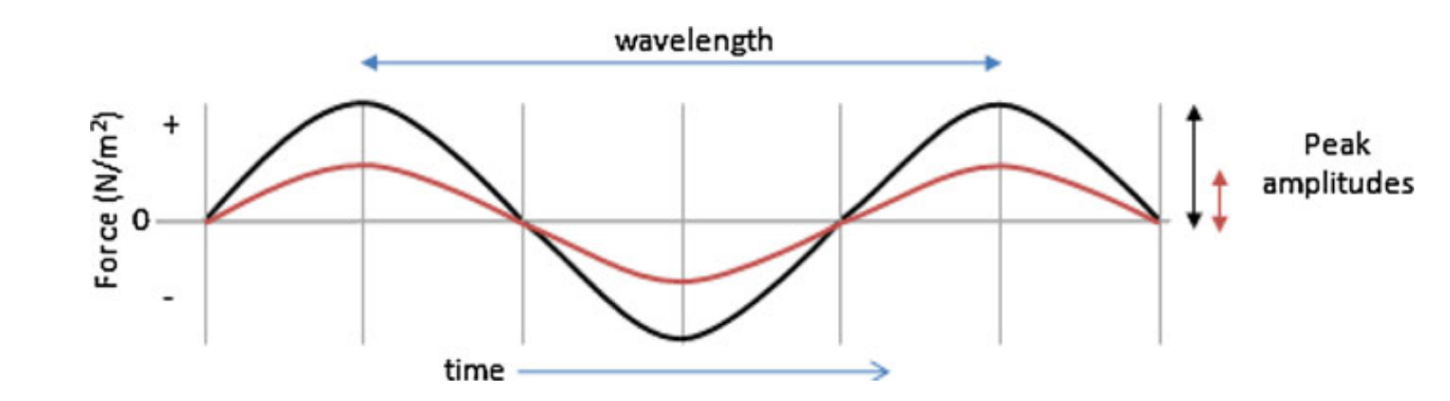
\includegraphics[width=0.85\textwidth]{wave} \\[12pt]
\end{center}
\cite{villanueva}
When we take a closer look at waves, certain similarities amongst all waves start to appear. These characteristics can be used to describe waves and how they interact with their environment. The most prominent feature is that simple tones are comprised of simple sinusoidal waves. These are generally graphed as the force of pressure over time. Once graphed, the wavelength of a wave can be measured. This measurement shows the distance between the peak forces over time. One wavelength can be understood as one cycle of the wave. The amount of cycles that appear per time unit can be described as the frequency of the wave. A higher frequency wave correlates to a higher ``pitch'' when heard. Another correlation between these graphed waves and sound is the height of wave peaks. The higher the wave peak, the louder the sound is. The ``loudness'' of a sound is measured in decibels (dB), which are measured in log 10 units. This measurement system is a reference system, with 0 being the minimum value that a healthy human can hear.\cite{villanueva}
\begin{center}
  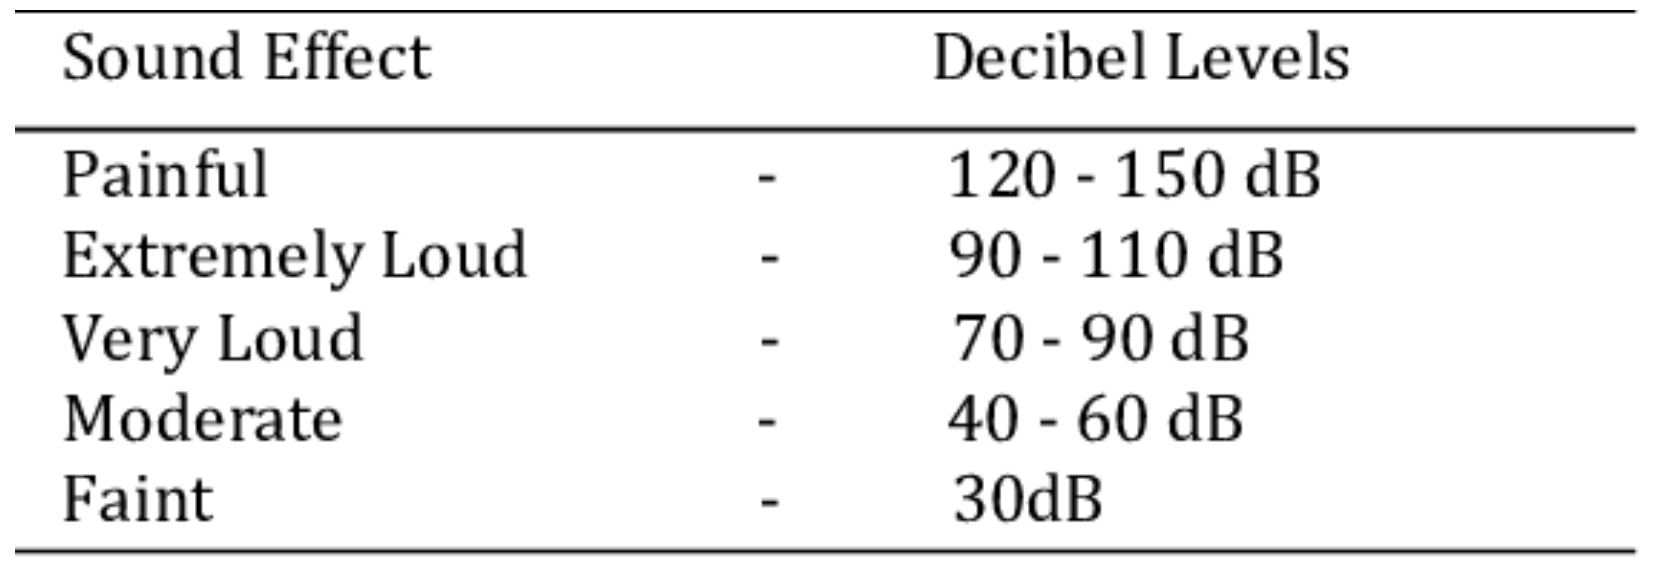
\includegraphics[width=0.85\textwidth]{soundChart} \\[12pt]
	\cite{sound}
\end{center}

\subsubsection{Interferences in Sound}
Sound waves can vary greatly in frequency, ranging from lower pitches around 20 Hz up to super sonic sounds at 60 kHz. The frequency at which a sound is produced greatly influences how it is affected by the environment through which it travels. High frequency sounds have a tendency to be absorbed by obstructions in the environment, such as leaves, and obstructions by nature limit the range at which high frequency sounds can travel. In contrast, lower frequency sounds have more ``flexibility'' and can move through more obstructions in an environment, allowing them to travel much further than high frequency sounds. This leads to very different sound profiles depending on the geographical location in which observations take place.\par
We use tools called spectrograms in order to visualize these discrepancies. It is important that, when conducting research in soundscape ecology, we keep in mind how the physical environment will block the more delicate higher frequency sounds from the observer. This is usually counteracted by using multiple recording devices placed in equidistant patterns that cover the area of interest. Using this technique allows recording devices in better positions to pick up on sounds that obstructed devices might miss.

\subsubsection{Spectrograms}
\begin{center}
  \includegraphics[width=0.85\textwidth]{spectrogram} \\[12pt]
\end{center}
It is not uncommon in soundscape ecology to see images as the one pictured above. These graphics are called spectrograms, and they allow soundscape ecologists to visualize frequencies over time. A spectrogram is read from left to right following the passage of time. Moving up the $y$-axis shows a linear increase in frequency and a corresponding increase in pitch. The darker colors show the intensity of a sound at that particular sound range. The lighter the color the softer the sound at that frequency is. The colors depend on what spectrogram one is looking at, but there should be a legend on the side describing the nuances of each specific graph. It is common for some indices (more information in the Soundscape Ecology Indices section) to divide the spectrogram into bands of frequencies. These bands are then compared by ratios to pull out the diversity of a certain sound clip.\par
The mechanism by which complex sound waves are turned into bands of frequency is central to how soundscape ecology is conducted, and so it is beneficial to have at least a basic understanding of the process. At the heart of it is the Fourier transform.\par
When we have a complicated wave created by many simple notes (simple meaning single frequency), what we experience is the addition of the two waves over a period of time. If one wave is in a descending crest while the other is ascending, then the addition is destructive. On the other hand, if both waves are cresting at the same point the interference is said to be constructive. The addition of these two waves destroys the sinusoidal nature and creates a brand new wave type. This new wave has no single frequency and thus cannot be easily displayed onto a spectrogram. This is where the Fourier transform comes into play.\par
To begin our transform we start by mapping the wave function from Cartesian coordinates to polar coordinates, as shown below.
\begin{center}
  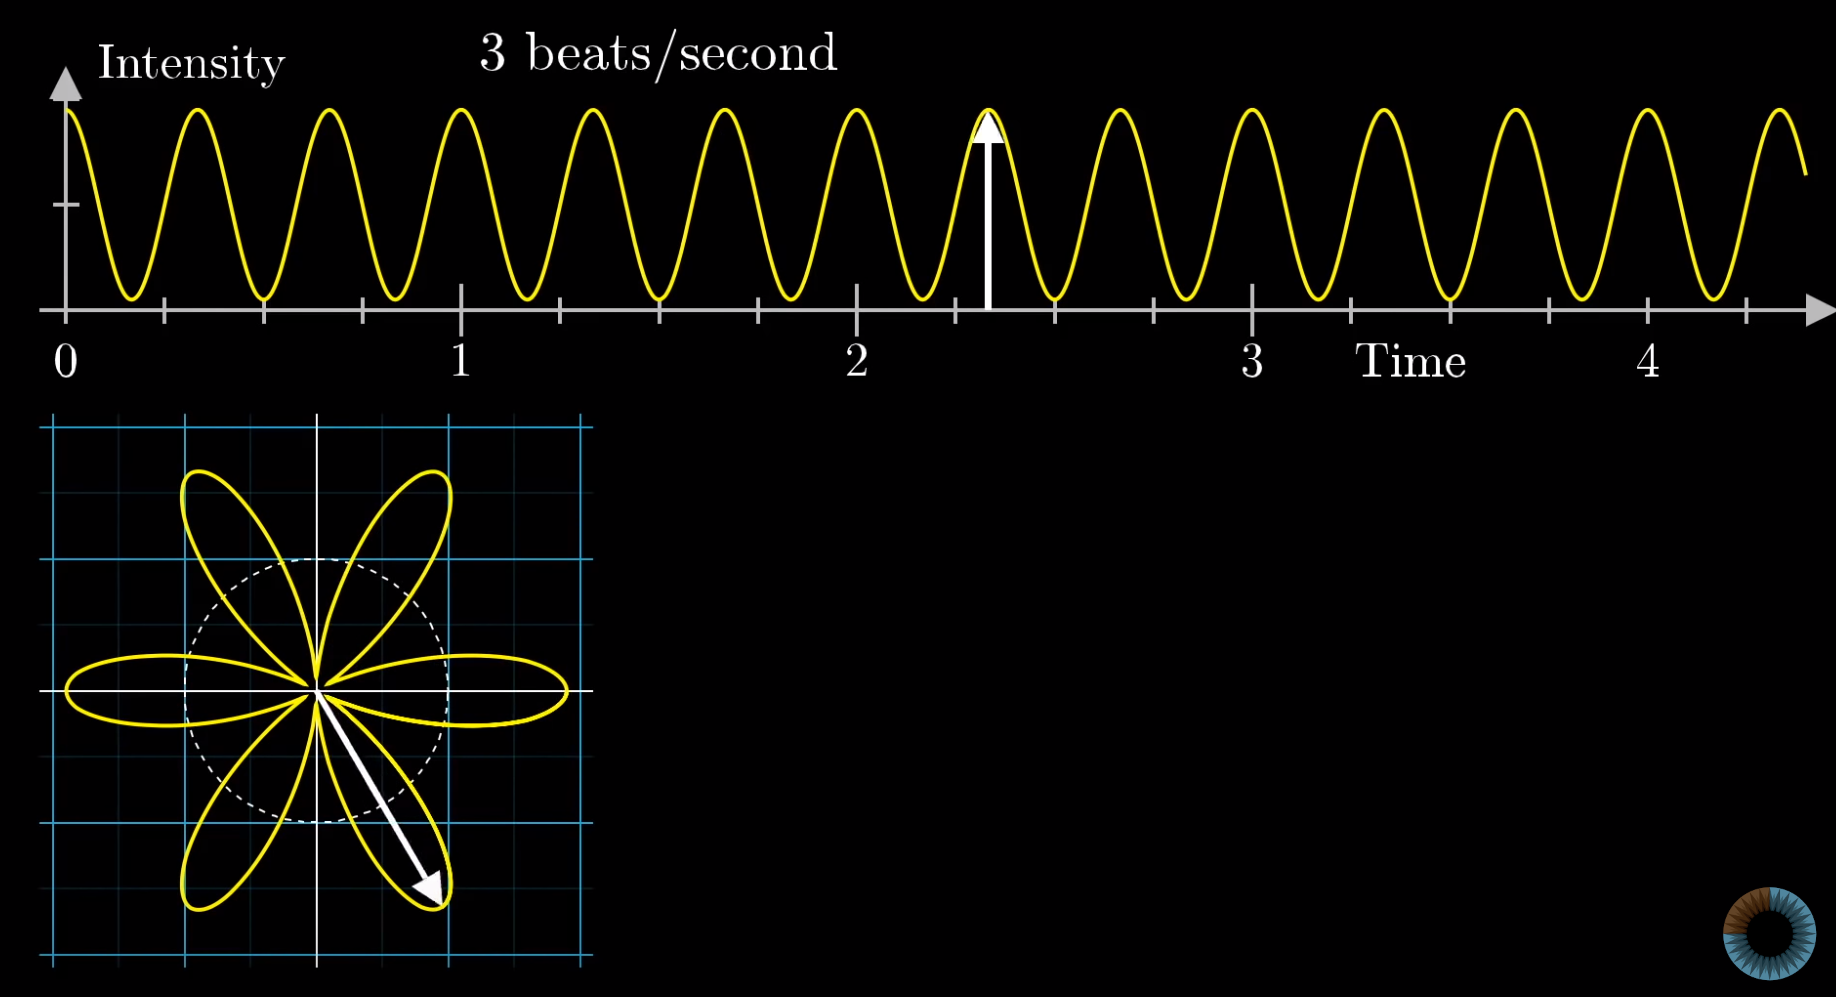
\includegraphics[width=0.85\textwidth]{polar} \\[12pt]
\end{center} \cite{bluebrown}
In the above example, the wave is plotted on the polar axis at the rate of 0.5 cycles per second. This rate can be changed, and changing it will effect how the polar coordinate graph will appear. The trick here is that if the rate at which you plot the wave onto the polar axis coincides exactly with the frequency of the original wave then the ``center of mass'' of the polar graph shifts outwards. This shift represents the intensity of a sound at that frequency. Not only can this change in the center of mass tell which frequency tones make up the original complicated wave, but it can also tell the intensity of specific frequencies within that wave. Using this, it is possible to directly map the original wave to a spectrogram. Using the $x$ position of the center of mass of the polar coordinate graph to show the intensity of a frequency, choosing the frequency is as simple as changing the cycles per second at which the graph drawn, 3 cycles per second being 3 Hz, 10 cycles per second being 10 Hz, and so on.
\begin{center}
  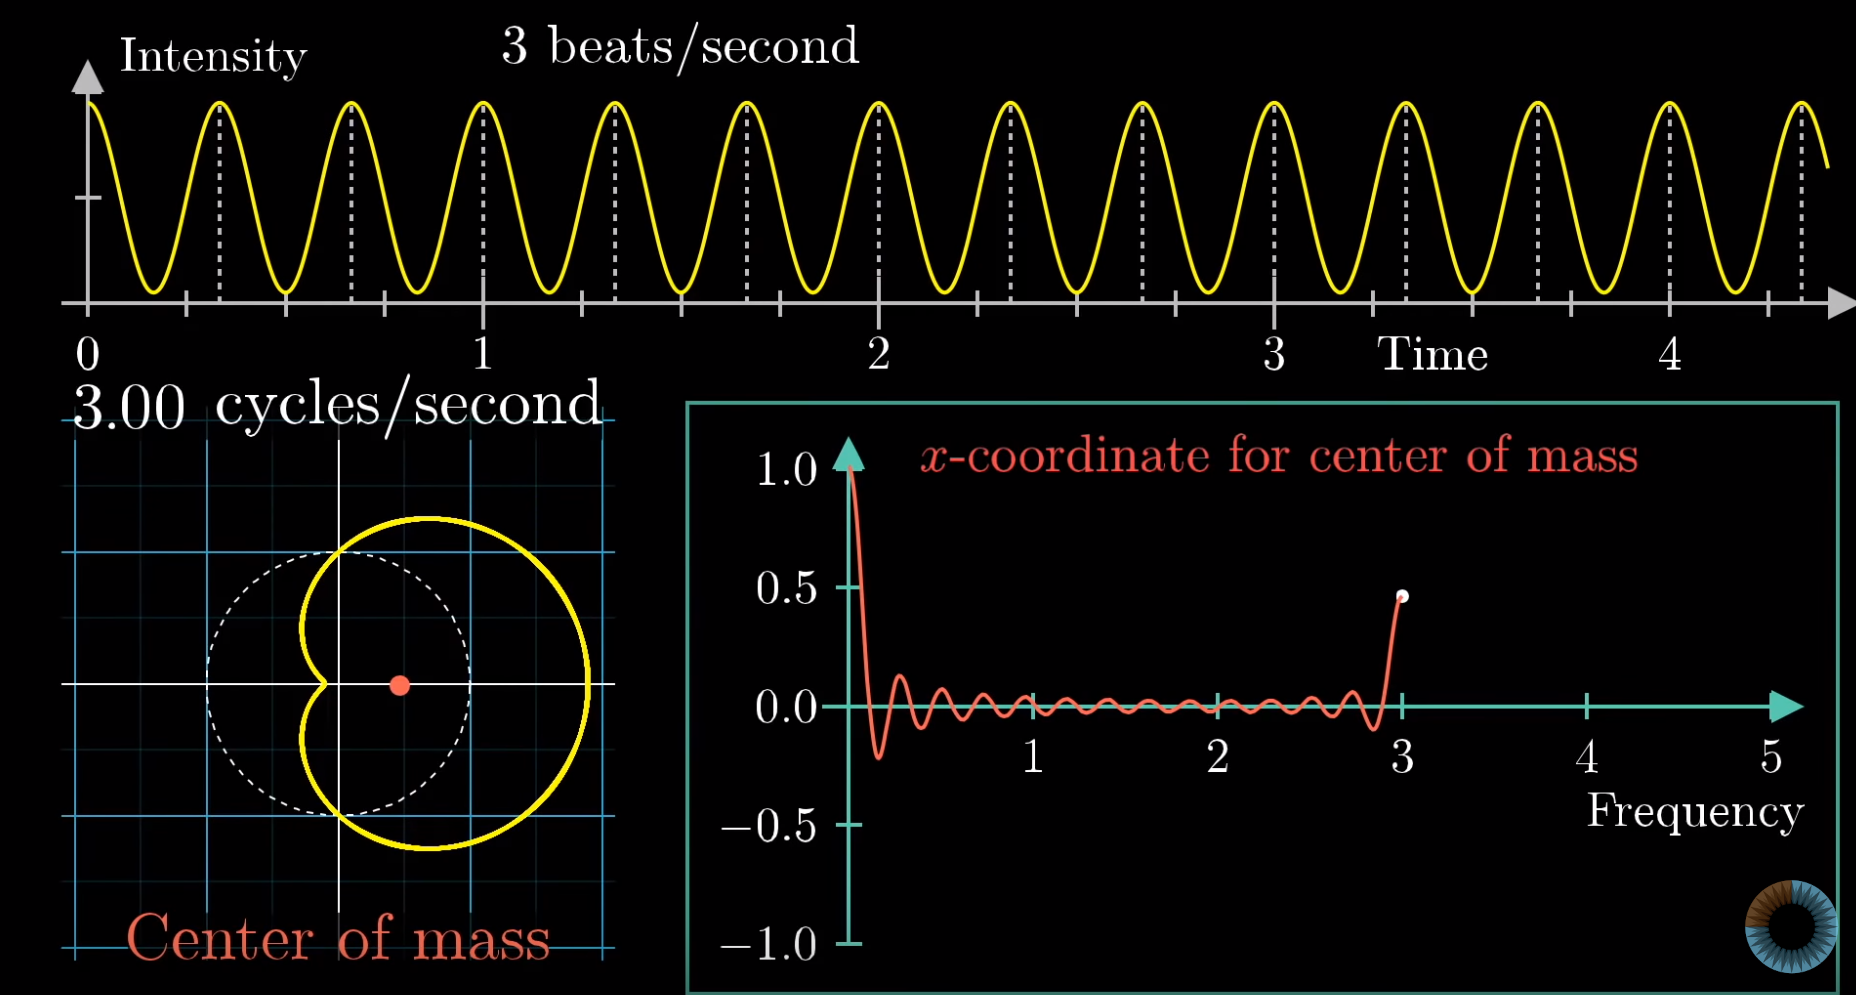
\includegraphics[width=0.85\textwidth]{centerofmass} \\
\end{center}
\begin{center}
  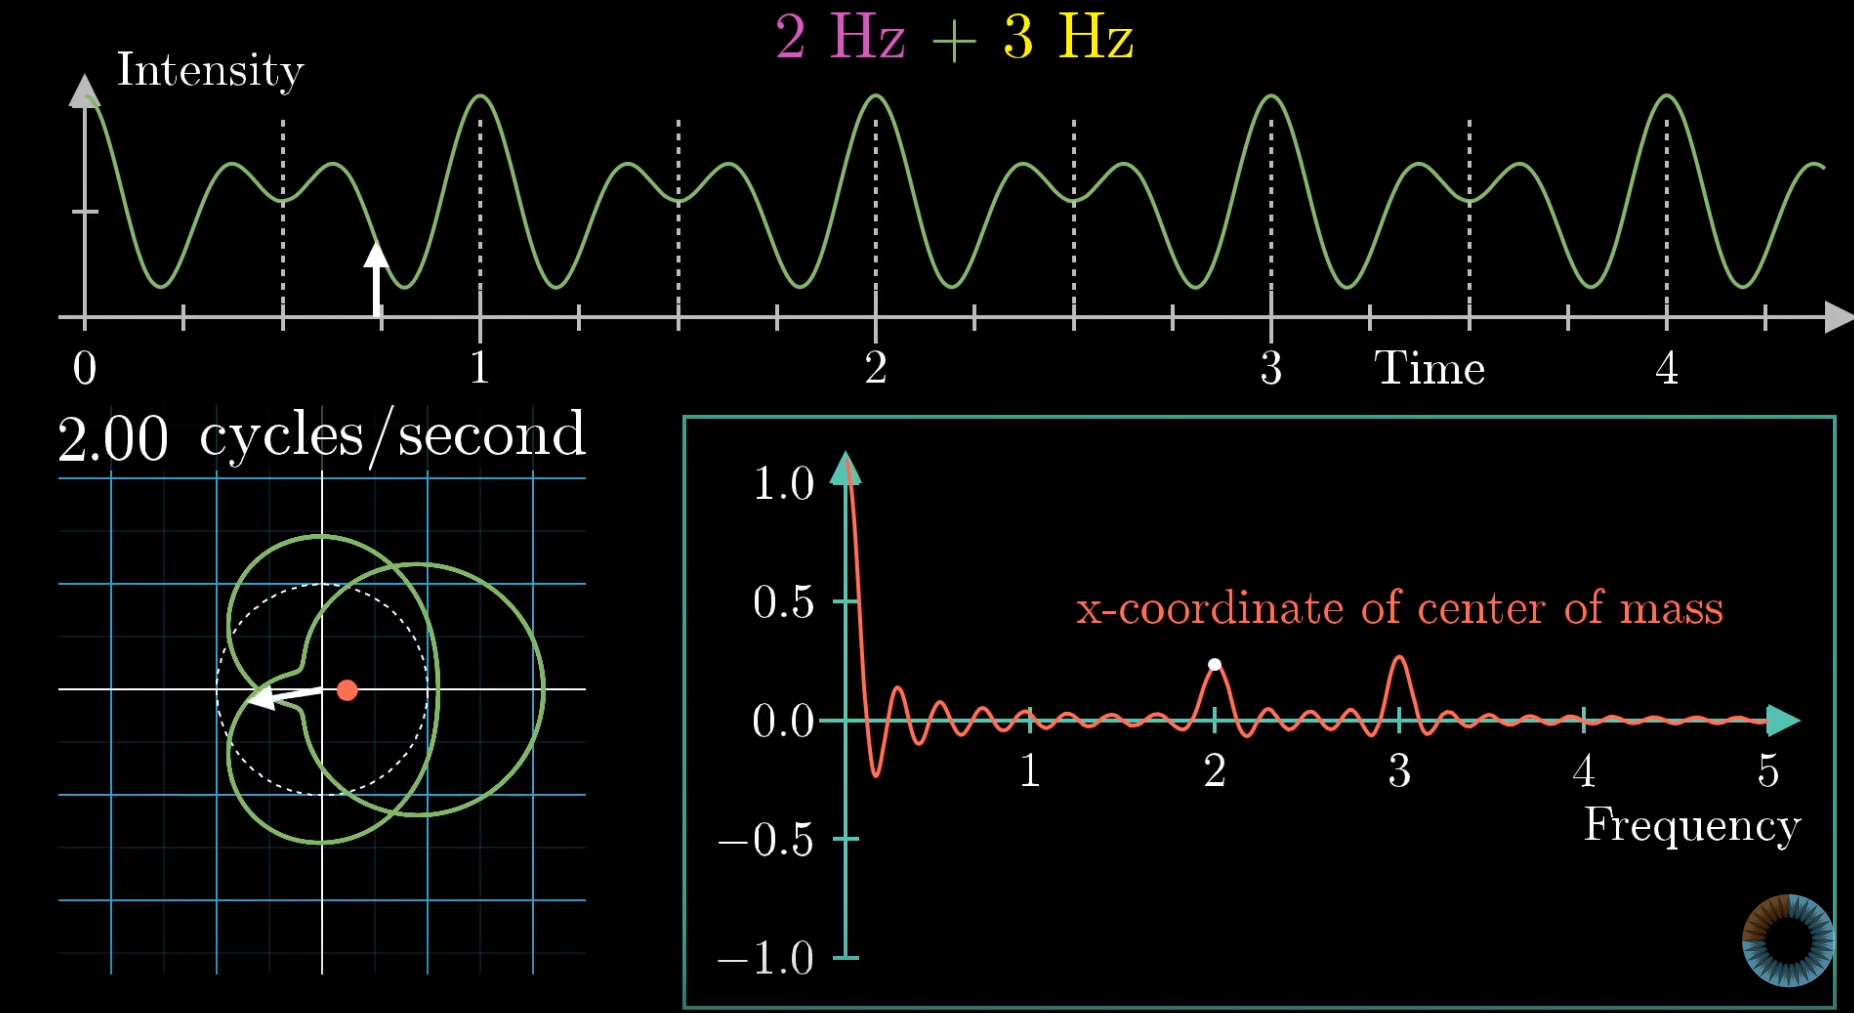
\includegraphics[width=0.85\textwidth]{shiftedcenter} \\[12pt]
  \cite{bluebrown}
\end{center}
This intuitive idea can then be boiled down to a single equation, which comprises of the integral over the initial wave function with Euler\textquotesingle s number to take into account the cyclical nature of the function. The equation is as follows \cite{bluebrown}:
\begin{equation}
  \int_{t_1}^{t_2} g(t)e^{-2\pi i f t} dt
\end{equation} \\[\eqnspace]

  \begin{center}
II. Soundscape Indices
\end{center}
\begin{flushleft}
\setlength{\parindent}{0.125in}
The \codesnip{soundecology} R package was developed by Luis Villanueva. This package contains algorithms for calculating the major indices, along with some extra abilities. Obviously, each algorithm outputs the index value, however each also outputs specific values, value lists, and matrices that are also used heavily in this service for creating the visualizations.\par

\noindent\textit{A. Acoustic Complexity Index}\par
The ACI, in combination with other measuring techniques, can be a powerful tool for finding the Biophonic sounds within a recording. ACI relies on the fact that most Biophonic (non-human biological sounds) have a high level of complexity when it comes to their intensity. Meaning that most natural sounds have a high variance of loudness. This is in stark contrast with the mostly monotone nature of human made sounds. This key difference in sound types allows the ACI to filter out plane noises or car sounds amongst bird sounds and other Biophonic interests. While there is a promising amount of research for the ability of the ACI to discriminate between Anthrophony and Biophony, the algorithm still does very poorly in discerning between different types of Biophony and Geophony. This challenge can be highlighted by the fact that the algorithm produces high numbers for sounds such as buzzing insects and wind.\par

\noindent\textit{B. Normalized Difference Soundscape Index}\par
One goal within the field of soundscape ecology is the analysis of the key characteristics of the Anthropocene, that is, the impact that humans have on wildlife and Earth as a whole. And perhaps no other metric of analysis symbolizes this better than the NDSI. NDSI has the goal of measuring the ratio between anthropogenic sounds and biological sounds.\par
The basis of this metric originates from a 2004 thesis written by Brian Michael Napoletano entitled \textit{Measurement, Quantification and Interpretation of Acoustic Signals Within an Ecological Context.} In this paper, Napoletano proposed three classifications for the sources for domains of sound frequencies: geophony (full spectrum), anthrophony (0 to 2 kHz), and biophony (3 to 11 kHz).\cite{napoletano} By ignoring potential geophony (as it would occur over too wide of a spectrum to identify), NDSI measures the acoustic energy (in watts) produced within the anthrophony and biophony spectrums.\par
Of course, this metric has its limits. In addition to completely ignoring all signals of geophony, NDSI fails to take into account variations in acoustic energy patterns depending on the source of sound, the time of day, and the season.\par

\noindent\textit{C. Bioacoustic Index}\par
The bioacoustic index was originally developed by ecologists studying the effects of invasive species on the native bird population of Hawaii. The purpose of such an index was to create a metric that closely correlated to the actual population of birds within an environment. This way, the researchers could have a reasonable estimation of the amount of birds within a given area without having to count them all by hand all the time.\par
This metric works by first specifying a range of frequencies (in Hz) at which biophony (or just about any type of sound that researchers expect to target) is expected to occur. Then, within this range of frequencies, measure the power (in Db) produced from these recordings within bins of specified ranges of time (in s). This should result in a collection of segments of curves of power. Finally, through determining the average area underneath these curves, the bioacoustic index value is found.\par
Of course, however, this metric has some drawbacks. Namely, it requires knowledge of the environment that the field work is occurring in. In order for this metric to be used effectively, researchers need to know beforehand the frequency range they intend to target and the correlation factor between the actual population count and the bioacoustic index value.\par

\noindent\textit{D. Acoustic Evenness and Diversity Index}\par
The ADI (Acoustic Diversity Index) bases its numerical evaluation on the concept of evenness of a set. A statistical theory first appearing in the 1960\textquotesingle s it is used to measure the diversity of a set of data.\par
One of the great features of the ADI using the Shannon-Wiener index is that it is not greatly affected by sample size. Along with that the ADI can capture a lot of information in one expression. Which can be helpful to express data to a general audience. That being said you must put this index into context. Mainly one must state the range of values that the index can output. These minimum and maximum values put the output value into context for the data collected. Just like most indices it is important that diversity indices are used along other measures. This allows for a holistic measure of the state the environment is in.\cite{shannonWiener}\par
While the method of taking individual sounds of birds and using ratios of specific calls is much more accurate, it is very difficult to identify individual calls in an automated fashion. Thus, when using a script to calculate the evenness or diversity of a sound clip, bands of frequencies are often used.

\end{flushleft}

  \subsection{Soundecology R Package Research}
The \codesnip{soundecology} R package was developed by Luis Villanueva. This package contains algorithms for calculating the major indices, along with some extra abilities. Obviously, each algorithm outputs the index value, however each also outputs specific values, value lists, and matrices that are also used heavily in this service for creating the visualizations.

\subsubsection{ACI Algorithm}
The ACI algorithm outputs more useful information than most of the other algorithms. In addition to the base ACI value, it outpus an ACI value by minute, which is a bit better representation of the ACI, especially for longer files. It also outputs a list of ACI values for each bin, which all sum up to the total ACI value. This list is useful for creating the line graphs included in this service. More information on the ACI index can be found in the Overview of Indices section.

\subsubsection{NDSI Algorithm}
The core NDSI algorithm that comes with the soundecology package outputs everything needed for this service, so no changes are needed. Those outputs include the NDSI values for both channels, as well as the biophony and anthrophony for both channels. These values are used for the visualizations, expanded upon in the Data Visualizations Research section.

\subsubsection{ADI and AEI Algorithm}
As ADI and AEI are closely related, their outputs are mostly the same, just tailored to the respective index. Along with the actual ADI or AEI value, the algorithms also output the ADI or AEI value for each band range, which is not included natively for AEI in the R package, and is included in the Proposed Changes section. These values include the ADI or AEI value at each frequency range, which can be specified by the user when creating jobs. Using these outputs, the ADI and AEI charts are able to be made.

\subsubsection{Bioacoustic Index Algorithm}
For the Bioacoustic index, the outputs for this service also include the left and right values, as well as the left and right normalized values for each frequency range. This is different than the base \codesnip{soundecology} package, and these changes are explained in the Proposed Changes section. For more information on how the Bioacoustic index is calculated, see the Overview of Indices section.

\subsubsection{Soundecology Package Dependencies}
The core soundecology package does not handle wav file conversion to Wav object that is needed for use in the algorithms. This is handled by a package named tuneR, which takes in audio files and converts them to R objects compatible with the R algorithms in soundecology. This is the only package that is of any note, as it will require its own set of instructions during our processing of the user\textquotesingle s files. The script for converting a user file into a Wav object is the following

\begin{javascriptcode}
  tdir <- getwd()
  tfile <- file.path(tdir, "SoundFileName.wav")
  newWobj <- readWave(tfile)
  result <- ndsi(newWobj)
\end{javascriptcode}

In order for this to work, the current working directory must be set to where the user\textquotesingle s files are located, and the SoundFileName must match the user\textquotesingle s as well. Luckily soundecology \textit{does} have a method, multiple_sounds, for going through all files in a subdirectory, and handles this natively. However multiple_sounds only goes through a directory, not for single file use.

\subsubsection{Proposed Changes}
For use in our service, this R package needs to be modified. Namely, the Bioacoustic index and AEI outputs need to be more detailed. For Bioacoustic, the bioacoustic values for both the left and right channels need to be output, along with the normalized left and right channel values. These values are in turn used in our visualizations to create the area graphs shown in the Data Visualizations Research section. As for AEI, it just needs to be changed to match that of the ADI. For whatever reason, the core package outputs only the AEI values for the left and right channel, and did not output the left and right band values and left and right band ranges. These are also used in the AEI and ADI visualizations.\par
Another proposed change that is talked about a bit in the Benchmarking section, is that of file size constraints. Currently, certain indices are not able to be computed on long files due to hardware limitations even on high end systems. These memory issues are the result of matrices being created in indices like ACI. From reviewing the code, these matrices are being used as intermediary values used in the calculation of lists of \textit{more} intermediary values. These matrices are in fact output to the user, however the usefulness of them is up for debate. Proposed changes to circumvent these issues include possibly removing these matrices, or adding a file splicing feature. Files that are over a certain length would need to be split into equal length parts, and the index would be calculated on each. From there, the overall index value could be calculated either in R or in the client.


  \subsection{Data Visualization Research}

  \newpage

  \section{Conclusions}
  \subsection{Project Progress and Successes}
\subsubsection{Tools for Success}
Our meeting schedule changed throughout the two semesters based on the needs of the project. During the initial design process, we met at least weekly along with daily Discord discussions. These weekly meetings lasted until we all felt we had made a considerable amount of progress on the project. Once most of the design decisions had been made and we decided to start working on the application, we met on an as needed basis. At this point, Discord communication became more frequent. We created Discord channels related to certain areas of the project, like backend, frontend and a channel to discuss ideas and plans for writing this design document. Documents related to the design process are stored in a shared Google Drive folder. Github has been used for our frontend and backend code, as well as our \LaTeX{} design document.\par
Our team manager has kept up with setting topics and goals before each meeting, as well as keeping track of ideas discussed in meetings. These are also kept in our Google Drive folder. This practice also allows us to keep track of our progress and evaluate if we are behind schedule on any part of the project.\par
We have kept values in mind during design and development. This includes making sure we are considering the needs of our sponsor and future users.\par
The concept of creating 100 ideas has been done throughout our team meetings and Discord communication, with lengthy discussions becoming commonplace in the early stages of this project. This is especially true when thinking about design decisions, many ideas are suggested in our meetings until the team has agreed that the best ones have been found. We have dealt with risks in a similar way to the 100 ideas method. By trying to think ahead to potential risks that may arise in the future, we were able to plan around them or think of a new idea so that the risk could be avoided.\par
Delegating tasks has been a very useful practice throughout our project. This has aided in the design process by splitting up sections of the design document across our team. New ideas were discovered and discussed in meeting and by doing this we have been able to cover more material. In development this has also been useful, as our team is split up into frontend and backend with subroles within each group, ensuring that no aspect of the project is forgotten.\par

\subsubsection{Milestone Progress}
\paragraph{Phase 0 - Requirement Gathering and Initial Design} \mbox{}\\[\paragraphheaderspace]
The first milestone in this section, gathering requirements has been completed throughout various meetings with our team, sponsor, TAs and professor. Discussions with our sponsor have clarified what it means for our project to be successful and determined which features should be considered stretch goals. In meeting with our professor, the importance of attempting to implement stretch goal features has been discussed. Our team has agreed on pursuing machine learning  and collaboration stretch goals and we have allocated time for this as shown in the Milestones section of this paper.\par
The aspects of project design, including the database, API/backend and frontend have been through various iterations and continued to improve throughout the project. A more detailed account of this process can be found in the Design Iterations section of this document.\par
\paragraph{Phase 1 - Research and Prototyping} \mbox{}\\[\paragraphheaderspace]
We made a good amount of progress prototyping our server and client applications compared to the milestone dates set at the start of semester one. Progress on the server side application included some API requests. The backend team continued to develop the requests outlined in the Application Programming Interface section.\par
Prototyping of the client application was also off to a good start. The application runs on Electron in a development environment and the front end team made progress on pages of the application. The client prototype application had a navigation panel for each of the pages that have started to be implemented, job creation, job queue and catalog.\par
Progress on the catalog page included job filtering and searching. On this page, progress on Recharts visualizations for results had also been made for all indices and data structured the way it will be in the database could be viewed in Recharts graphs. By the end of December, these two features were working together by showing job results of any sample job searched, as well as job comparisons. The job queue page, where a user starts new jobs, included UI selection of indices and parameters. The next step on that page was file input selection for jobs and after that was implemented, requests could be sent to the API to make a new job.\par

\paragraph{Implementation and Stretch Goals} \mbox{}\\[\paragraphheaderspace]
Implementation of the local desktop application began in early January. After all aspects of the client application were functioning with sample data, we started to include API requests to get both applications working with one another. The backend team continued to create more of the necessary requests for our application while the front end team worked with sample data. We were successful in meeting the date set in the milestones section, January 25, 2018, for the implementation of the desktop application. Some backend testing had also already taken place at that time.\par
Implementation of the AWS backend application may be the only section that we underestimated the time needed to complete in our milestones. Because of this it was decided to move this portion of the project into stretch goals.\par
Stretch goals were not been our primary concern, in order to get all required goals completed first. We have had one designated member of our team researching possible implementations of our stretch goals through machine learning. When the required features were completed, the rest of the team would be able to move their focus to this area and the research already done would serve as a good starting point. However, due to increased time spent working on more advanced features in the frontend, this work stayed with just one group member.\par

\paragraph{Sponsor Feedback and Additional Features} \mbox{}\\[\paragraphheaderspace]
After the API was fully implemented, files were able to be processed and the client application could use real data given by the results of running jobs. After all major features were complete, Mangrove was set up on our sponsor\textquotesingle s computer and we were given feedback and suggestions for additonal features on both the client and server applications. We shifted our focus to implementing this feedback, as well as correcting any bugs found.\par
Progress made on the client application during the second semester include researching and implementing the most useful visualizations for results of each type of job and adding the ability to playback audio when a data point is clicked. Automating the collection of metadata from the names of sound files was added to improve the user\textquotesingle s experience by the request of our sponsor. Other client features completed in the second semester include exporting results to CSV files and live updates of graphs as jobs are processed. The login page was also completed, along with user authentication and persistent user sessions.\par

  \subsection{Stretch Goals Success and Difficulties}
As outlined in the Milestones report of this document, most of the stretch goals of this project were not reached. While stretch goals are set to be above and beyond goals, we aimed to fulfill them and even expected to in some capacity. The purpose of this section is to outline these stretch goals and the successes and difficulties faced during development. Additionally, this section serves to provide guidance to future work as to how to accomplish these stretch goals.\\

\subsubsection{Machine Learning}
Machine listening is a highly demanding task. Not only is it technically difficult, but it also requires a much higher processing power than other forms of ML. During similar model development, models took around 7 hours to train. While libraries exist for ML with sounds, the most promising one only works in real time, in that it listens as sounds are made to make predictions. This is is technically what we were aiming to include with Mangrove, it may be useful in the future should Mangrove go mobile in some capacity.\cite{EARS}\par
One approach that was going to be taken for ML was using index outputs as features to predict if the recording contained a bird. We would be using the sound files included in the Cornell library purchased for this project, however we also needed sound files that were not birds. Ultimately, the issue of file formatting was introduced, and simply converting mp3 to wav did not allow the indices to be run on the converted files. This effectively ruined this approach. In order for this to work, the files containing the bird sounds would need to be originally recorded in the wav format, along with the non bird sounds. The man power to do this recording is simply not available in the scope of this project.\par
While we did run into some major difficulties some progress was made with the research, as can be seen in the machine learning section. Along with some preliminary testing on Vanilla Neural Networks, we also established some common place feature extractors used in the field. Through our research we found the MFCC log scale and ConvRBM\textquotesingle s to be the most widely used. With the former achieving over 75\% accuracy with a CNN classifier.\par
Along with identifying methods of feature extraction and rough model architectures, we have also made some progress in the data collection space. We've compiled a labeled directory of cornell bird sounds and a collection of urban noise from the EC-50 dataset.\cite{soundData} Our data set could be used as a comprehensive noise space of sounds that researchers may run into while listening in areas like UCF; that have a mixed soundscape of both anthrophonic and biophonic sounds. Along with this dataset we have done some work with web scraping in order to download insect sounds. We were able to collect over 100 sounds from online sources.\cite{ot} This method can be further deployed by future groups in order to obtain more data from various species.

\subsubsection{Collaboration Abilities}
We, along with our sponsor, wanted to include some sort of collaborative abilities with Mangrove. The purpose of this was crowd sourcing data surrounding soundscape research, to see what kind of sounds and data were coming out of different places around the country. In addition, intra facility research collaboration was intended, and is elaborated on more in the next section.\par
The backend has been designed with this functionality in mind, and is primed for future work to be done to implement collaboration. However as development continued in our time working on Mangrove, more features pertaining to the core functionality of the program were thought of and implemented. Features like audio playback, data exporting, and ensuring that the graphs were correctly presenting data felt paramount to the core of this project, and were taken to before collaboration was designed, at least in the frontend.\par
The vision of collaboration on a grand scale like we intended included an AWS backend for storing user data that can be accessed by anyone using the service. The users could choose which data to upload for the sake of open source data and research. A chloropleth map was going to be included as a heat map of where the most research and sounds were coming from through out the country. Our sponsor Dr. Beever is very interested in crowd sourcing data and open sourcing both research and this program for anyone to use, so collaboration abilities seem the next step in the future of Mangrove.\\

\subsubsection{Research Groups}
Our sponsor mentioned that at places like Purdue University, there are large research groups in the field of soundscape ecology. This sparked the idea of allowing for research groups to be created in Mangrove, aiming to help organize group sound files and data by author. This is a type of collaboration, but in a more private way. A user could create a research group for themself, becoming an admin. From there, they could add other users to their research group. Doing so would allow for a few permissions between the members of this research group. Assuming the group is using a central dedicated server for storing and processing their sound files and results from Mangrove, any group member could access these sound files that belonged to the group. Additionally, any group member could access the results from jobs run by other group members. In the client, when viewing input files and jobs, any member can see the author of both the sound file and the job.\par
This feature along with the global collaborative abilities seem central to the future of Mangrove. We hope that as soundscape ecology becomes a bigger area of research, Mangrove becomes the core data organization and processing software for researchers. For this to happen, research group abilities along with user account abilities must happen.\\

  \subsection{Final Remarks}
Some of the major successes that come with Mangrove include the fact that this piece of software really is one of a kind. There is no known software available solely for soundscape ecology researchers to both organize and process their datasets. One of the features that makes this possible would be the graphs that come along with Mangrove. Finally, researchers have access to visuals that describe the numbers they are currently forced to work with. The vision is that in using these graphs, researchers can now publish their findings in a consumable fashion for both other researchers and the general public. Another great feature of Mangrove is the processing capabilities. Before, researchers like our sponsor would have to work in the terminal to run R scripts that had the potential to fail and nullify any progress made. Now, each file is run with live updates to show the user that work is actually happening. Just because one file may have failed doesn\textquotesingle t mean that the entire operation is now botched. Providing an intuitive interface for researchers to use these algorithms to analyze their sound files is a valuable resource in this blooming field.\par
Aside from the technical achievements of Mangrove, through development we have also brought to light some challenges and discrepencies in the field of sound ecology. We have been able to identify problems in the algorithms being used by researchers and are able to propose changes (and have made changes even) to the algorithms to improve validity of data. Additionally, our machine learning research has shed a great deal of light on the possibilities of machine listening and the implications of that practice as it pertains to soundscape ecology research.\par
Moving forward, we hope that the collaborative abilities planned by our current design are brought to fruition. The ultimate goal of Mangrove is to be open source and public facing in order to promote open data in the realm of soundscape ecology. We also hope that the research done regarding the index algorithms and their validity and purpose in the field is found useful to researchers, as we feel there is a great deal of discrepency as to the actual usefulness of these algorithms. Finally, we hope that machine learning is integrated into Mangrove in the future using the research and work done in our two semesters working with it.\par
Overall, Mangrove has been a great success. Crunch time was minimal, and the requirements we set out to reach have been met. We feel that Mangrove has provided everything our sponsor wanted and then some, and we know that both him and our team are proud of the work done on Mangrove.\par

  \newpage

  \thispagestyle{empty}
  \printbibliography
\end{document}
